\documentclass[twoside]{book}

% Packages required by doxygen
\usepackage{fixltx2e}
\usepackage{calc}
\usepackage{doxygen}
\usepackage[export]{adjustbox} % also loads graphicx
\usepackage{graphicx}
\usepackage[utf8]{inputenc}
\usepackage{makeidx}
\usepackage{multicol}
\usepackage{multirow}
\PassOptionsToPackage{warn}{textcomp}
\usepackage{textcomp}
\usepackage[nointegrals]{wasysym}
\usepackage[table]{xcolor}

% Font selection
\usepackage[T1]{fontenc}
\usepackage[scaled=.90]{helvet}
\usepackage{courier}
\usepackage{amssymb}
\usepackage{sectsty}
\renewcommand{\familydefault}{\sfdefault}
\allsectionsfont{%
  \fontseries{bc}\selectfont%
  \color{darkgray}%
}
\renewcommand{\DoxyLabelFont}{%
  \fontseries{bc}\selectfont%
  \color{darkgray}%
}
\newcommand{\+}{\discretionary{\mbox{\scriptsize$\hookleftarrow$}}{}{}}

% Page & text layout
\usepackage{geometry}
\geometry{%
  a4paper,%
  top=2.5cm,%
  bottom=2.5cm,%
  left=2.5cm,%
  right=2.5cm%
}
\tolerance=750
\hfuzz=15pt
\hbadness=750
\setlength{\emergencystretch}{15pt}
\setlength{\parindent}{0cm}
\setlength{\parskip}{3ex plus 2ex minus 2ex}
\makeatletter
\renewcommand{\paragraph}{%
  \@startsection{paragraph}{4}{0ex}{-1.0ex}{1.0ex}{%
    \normalfont\normalsize\bfseries\SS@parafont%
  }%
}
\renewcommand{\subparagraph}{%
  \@startsection{subparagraph}{5}{0ex}{-1.0ex}{1.0ex}{%
    \normalfont\normalsize\bfseries\SS@subparafont%
  }%
}
\makeatother

% Headers & footers
\usepackage{fancyhdr}
\pagestyle{fancyplain}
\fancyhead[LE]{\fancyplain{}{\bfseries\thepage}}
\fancyhead[CE]{\fancyplain{}{}}
\fancyhead[RE]{\fancyplain{}{\bfseries\leftmark}}
\fancyhead[LO]{\fancyplain{}{\bfseries\rightmark}}
\fancyhead[CO]{\fancyplain{}{}}
\fancyhead[RO]{\fancyplain{}{\bfseries\thepage}}
\fancyfoot[LE]{\fancyplain{}{}}
\fancyfoot[CE]{\fancyplain{}{}}
\fancyfoot[RE]{\fancyplain{}{\bfseries\scriptsize Generated by Doxygen }}
\fancyfoot[LO]{\fancyplain{}{\bfseries\scriptsize Generated by Doxygen }}
\fancyfoot[CO]{\fancyplain{}{}}
\fancyfoot[RO]{\fancyplain{}{}}
\renewcommand{\footrulewidth}{0.4pt}
\renewcommand{\chaptermark}[1]{%
  \markboth{#1}{}%
}
\renewcommand{\sectionmark}[1]{%
  \markright{\thesection\ #1}%
}

% Indices & bibliography
\usepackage{natbib}
\usepackage[titles]{tocloft}
\setcounter{tocdepth}{3}
\setcounter{secnumdepth}{5}
\makeindex

% Hyperlinks (required, but should be loaded last)
\usepackage{ifpdf}
\ifpdf
  \usepackage[pdftex,pagebackref=true]{hyperref}
\else
  \usepackage[ps2pdf,pagebackref=true]{hyperref}
\fi
\hypersetup{%
  colorlinks=true,%
  linkcolor=blue,%
  citecolor=blue,%
  unicode%
}

% Custom commands
\newcommand{\clearemptydoublepage}{%
  \newpage{\pagestyle{empty}\cleardoublepage}%
}

\usepackage{caption}
\captionsetup{labelsep=space,justification=centering,font={bf},singlelinecheck=off,skip=4pt,position=top}

%===== C O N T E N T S =====

\begin{document}

% Titlepage & ToC
\hypersetup{pageanchor=false,
             bookmarksnumbered=true,
             pdfencoding=unicode
            }
\pagenumbering{alph}
\begin{titlepage}
\vspace*{7cm}
\begin{center}%
{\Large Finance }\\
\vspace*{1cm}
{\large Generated by Doxygen 1.8.12}\\
\end{center}
\end{titlepage}
\clearemptydoublepage
\pagenumbering{roman}
\tableofcontents
\clearemptydoublepage
\pagenumbering{arabic}
\hypersetup{pageanchor=true}

%--- Begin generated contents ---
\chapter{Finance}
\label{md__users__c_u_i__dropbox__c_09_09__finance__r_e_a_d_m_e}
\hypertarget{md__users__c_u_i__dropbox__c_09_09__finance__r_e_a_d_m_e}{}
Financial Engineering

This repo is for my own practise using C++.

Instruction to link Quantlib with Xcode projects\+: 1. Target Project-\/$>$ Build Settings-\/$>$ Search Paths-\/$>$ Header Search Paths-\/$>$ /opt/local/include 2. Target Project-\/$>$ Build Settings-\/$>$ Search Paths-\/$>$ Library Search Paths-\/$>$ /opt/local/lib 3. Target Project-\/$>$ Build Phases-\/$>$ Link Binary With Library-\/$>$ + -\/$>$ lib\+Quant\+Lib.\+0.\+dylib (path\+:\char`\"{}/opt/local/lib\char`\"{}) 4. Target Project-\/$>$ Build Settings-\/$>$ Apple L\+L\+VM 7.\+1-\/\+Language-\/ C++-\/$>$ C++ Language Dialect -\/$>$ G\+N\+U++98\mbox{[}-\/std=gnu++98\mbox{]}

Instruction on incorporating github for source control 1. New a repo in github, say \char`\"{}\+Finance\char`\"{} 2. Create a new project in Xcode using the same name \char`\"{}\+Finance\char`\"{} for consistency. 3. In Terminal, open the \char`\"{}\+Finance\char`\"{} folder and intial the git file by git init 4. Link the local folder to the github website git remote add origin \href{https://github.com/scuiaa555/Finance.git}{\tt https\+://github.\+com/scuiaa555/\+Finance.\+git} 5. Grad the initial files on the github website git pull origin master git add $\ast$ git commit -\/m \char`\"{}\+Grab R\+E\+A\+D\+M\+E\char`\"{} 6. Add the files in local folder to the website git add Finance Finance.\+xcodeproj/ git commit -\/m \char`\"{}add project files to master\char`\"{} 7. Push to the server by using Xcode source control button Xcode-\/$>$ Source Control-\/$>$ Push Done. \+:) 
\chapter{Hierarchical Index}
\section{Class Hierarchy}
This inheritance list is sorted roughly, but not completely, alphabetically\+:\begin{DoxyCompactList}
\item \contentsline{section}{Generic\+Random\+Variable\+Generator\+:\+:Argument}{\pageref{class_generic_random_variable_generator_1_1_argument}}{}
\begin{DoxyCompactList}
\item \contentsline{section}{Generic\+Compound\+Poisson\+:\+:Argument}{\pageref{class_generic_compound_poisson_1_1_argument}}{}
\item \contentsline{section}{Generic\+Normal\+:\+:Argument}{\pageref{class_generic_normal_1_1_argument}}{}
\item \contentsline{section}{Generic\+Poisson\+:\+:Argument}{\pageref{class_generic_poisson_1_1_argument}}{}
\end{DoxyCompactList}
\item \contentsline{section}{Pricing\+Engine\+:\+:Arguments}{\pageref{class_pricing_engine_1_1_arguments}}{}
\begin{DoxyCompactList}
\item \contentsline{section}{Asian\+Option\+:\+:Arguments}{\pageref{class_asian_option_1_1_arguments}}{}
\item \contentsline{section}{European\+Option\+:\+:Arguments}{\pageref{class_european_option_1_1_arguments}}{}
\item \contentsline{section}{Forward\+:\+:Arguments}{\pageref{class_forward_1_1_arguments}}{}
\end{DoxyCompactList}
\item \contentsline{section}{Generic\+Random\+Variable\+Generator}{\pageref{class_generic_random_variable_generator}}{}
\begin{DoxyCompactList}
\item \contentsline{section}{Random\+Variable\+Generator$<$ return\+Type $>$}{\pageref{class_random_variable_generator}}{}
\item \contentsline{section}{Random\+Variable\+Generator$<$ double $>$}{\pageref{class_random_variable_generator}}{}
\begin{DoxyCompactList}
\item \contentsline{section}{Generic\+Compound\+Poisson}{\pageref{class_generic_compound_poisson}}{}
\begin{DoxyCompactList}
\item \contentsline{section}{Compound\+Poisson$<$ Poisson\+R\+NG, Jump\+R\+NG $>$}{\pageref{class_compound_poisson}}{}
\end{DoxyCompactList}
\item \contentsline{section}{Generic\+Normal}{\pageref{class_generic_normal}}{}
\begin{DoxyCompactList}
\item \contentsline{section}{Normal$<$ Norm\+Method $>$}{\pageref{class_normal}}{}
\end{DoxyCompactList}
\item \contentsline{section}{Generic\+Poisson}{\pageref{class_generic_poisson}}{}
\begin{DoxyCompactList}
\item \contentsline{section}{Poisson$<$ Poisson\+Method $>$}{\pageref{class_poisson}}{}
\end{DoxyCompactList}
\end{DoxyCompactList}
\item \contentsline{section}{Random\+Variable\+Generator$<$ vector$<$ double $>$ $>$}{\pageref{class_random_variable_generator}}{}
\begin{DoxyCompactList}
\item \contentsline{section}{Multi\+Rand\+Generator$<$ Args $>$}{\pageref{class_multi_rand_generator}}{}
\end{DoxyCompactList}
\end{DoxyCompactList}
\item \contentsline{section}{Instrument}{\pageref{class_instrument}}{}
\begin{DoxyCompactList}
\item \contentsline{section}{Asian\+Option}{\pageref{class_asian_option}}{}
\item \contentsline{section}{European\+Option}{\pageref{class_european_option}}{}
\item \contentsline{section}{Forward}{\pageref{class_forward}}{}
\end{DoxyCompactList}
\item \contentsline{section}{Mc\+Model$<$ R\+NG, Path\+Type $>$}{\pageref{class_mc_model}}{}
\item \contentsline{section}{Mc\+Simulation$<$ R\+NG, Path\+Type $>$}{\pageref{class_mc_simulation}}{}
\begin{DoxyCompactList}
\item \contentsline{section}{Mc\+Asian\+Engine$<$ R\+NG, Path\+Type $>$}{\pageref{class_mc_asian_engine}}{}
\item \contentsline{section}{Mc\+European\+Engine$<$ R\+NG, Path\+Type $>$}{\pageref{class_mc_european_engine}}{}
\end{DoxyCompactList}
\item \contentsline{section}{M\+C\+Statistics}{\pageref{class_m_c_statistics}}{}
\item \contentsline{section}{Model$<$ Type\+\_\+of\+\_\+single\+\_\+time $>$}{\pageref{class_model}}{}
\item \contentsline{section}{Model$<$ double $>$}{\pageref{class_model}}{}
\begin{DoxyCompactList}
\item \contentsline{section}{Model1D}{\pageref{class_model1_d}}{}
\begin{DoxyCompactList}
\item \contentsline{section}{Black\+Scholes\+Model}{\pageref{class_black_scholes_model}}{}
\item \contentsline{section}{Merton\+Jump\+Model}{\pageref{class_merton_jump_model}}{}
\end{DoxyCompactList}
\end{DoxyCompactList}
\item \contentsline{section}{Model$<$ vector$<$ double $>$ $>$}{\pageref{class_model}}{}
\begin{DoxyCompactList}
\item \contentsline{section}{Model\+ND}{\pageref{class_model_n_d}}{}
\begin{DoxyCompactList}
\item \contentsline{section}{L\+MM}{\pageref{class_l_m_m}}{}
\end{DoxyCompactList}
\end{DoxyCompactList}
\item \contentsline{section}{Multi\+Random$<$ R\+N\+Gs $>$}{\pageref{struct_multi_random}}{}
\item \contentsline{section}{Multi\+Variate}{\pageref{struct_multi_variate}}{}
\item \contentsline{section}{Multi\+Vol}{\pageref{struct_multi_vol}}{}
\item \contentsline{section}{Parameter}{\pageref{class_parameter}}{}
\begin{DoxyCompactList}
\item \contentsline{section}{Constant\+Parameter}{\pageref{class_constant_parameter}}{}
\begin{DoxyCompactList}
\item \contentsline{section}{Null\+Parameter}{\pageref{class_null_parameter}}{}
\end{DoxyCompactList}
\end{DoxyCompactList}
\item \contentsline{section}{Stochastic\+Process\+:\+:Parameter\+Set}{\pageref{class_stochastic_process_1_1_parameter_set}}{}
\item \contentsline{section}{Path$<$ Path\+Type $>$}{\pageref{class_path}}{}
\item \contentsline{section}{Path\+Generator$<$ R\+NG, Path\+Type $>$}{\pageref{class_path_generator}}{}
\item \contentsline{section}{Path\+Pricer$<$ Path\+Type $>$}{\pageref{class_path_pricer}}{}
\item \contentsline{section}{Path\+Pricer$<$ Single\+Variate $>$}{\pageref{class_path_pricer}}{}
\begin{DoxyCompactList}
\item \contentsline{section}{Asian\+Path\+Pricer}{\pageref{class_asian_path_pricer}}{}
\item \contentsline{section}{European\+Path\+Pricer}{\pageref{class_european_path_pricer}}{}
\end{DoxyCompactList}
\item \contentsline{section}{Payoff}{\pageref{class_payoff}}{}
\begin{DoxyCompactList}
\item \contentsline{section}{Vanilla\+Payoff}{\pageref{class_vanilla_payoff}}{}
\end{DoxyCompactList}
\item \contentsline{section}{Poisson\+Inverse$<$ Uniform\+R\+NG $>$}{\pageref{class_poisson_inverse}}{}
\item \contentsline{section}{Pricing\+Engine}{\pageref{class_pricing_engine}}{}
\begin{DoxyCompactList}
\item \contentsline{section}{Generic\+Engine$<$ Arguments\+Type, Results\+Type $>$}{\pageref{class_generic_engine}}{}
\item \contentsline{section}{Generic\+Engine$<$ Asian\+Option\+:\+:Arguments, Asian\+Option\+:\+:Results $>$}{\pageref{class_generic_engine}}{}
\begin{DoxyCompactList}
\item \contentsline{section}{Asian\+Option\+:\+:engine}{\pageref{class_asian_option_1_1engine}}{}
\begin{DoxyCompactList}
\item \contentsline{section}{Mc\+Asian\+Engine$<$ R\+NG, Path\+Type $>$}{\pageref{class_mc_asian_engine}}{}
\end{DoxyCompactList}
\end{DoxyCompactList}
\item \contentsline{section}{Generic\+Engine$<$ European\+Option\+:\+:Arguments, European\+Option\+:\+:Results $>$}{\pageref{class_generic_engine}}{}
\begin{DoxyCompactList}
\item \contentsline{section}{European\+Option\+:\+:engine}{\pageref{class_european_option_1_1engine}}{}
\begin{DoxyCompactList}
\item \contentsline{section}{Analytic\+European\+Engine}{\pageref{class_analytic_european_engine}}{}
\item \contentsline{section}{Mc\+European\+Engine$<$ R\+NG, Path\+Type $>$}{\pageref{class_mc_european_engine}}{}
\end{DoxyCompactList}
\end{DoxyCompactList}
\item \contentsline{section}{Generic\+Engine$<$ Forward\+:\+:Arguments, Forward\+:\+:Results $>$}{\pageref{class_generic_engine}}{}
\begin{DoxyCompactList}
\item \contentsline{section}{Forward\+:\+:engine}{\pageref{class_forward_1_1engine}}{}
\begin{DoxyCompactList}
\item \contentsline{section}{Analytic\+Forward\+Engine}{\pageref{class_analytic_forward_engine}}{}
\end{DoxyCompactList}
\end{DoxyCompactList}
\end{DoxyCompactList}
\item \contentsline{section}{Pricing\+Engine\+:\+:Results}{\pageref{class_pricing_engine_1_1_results}}{}
\begin{DoxyCompactList}
\item \contentsline{section}{Asian\+Option\+:\+:Results}{\pageref{class_asian_option_1_1_results}}{}
\item \contentsline{section}{European\+Option\+:\+:Results}{\pageref{class_european_option_1_1_results}}{}
\item \contentsline{section}{Forward\+:\+:Results}{\pageref{class_forward_1_1_results}}{}
\end{DoxyCompactList}
\item \contentsline{section}{M\+C\+Statistics\+:\+:Sample\+Results}{\pageref{class_m_c_statistics_1_1_sample_results}}{}
\item \contentsline{section}{Single\+Random$<$ R\+NG $>$}{\pageref{struct_single_random}}{}
\item \contentsline{section}{Singleton$<$ T $>$}{\pageref{class_singleton}}{}
\item \contentsline{section}{Singleton$<$ Normal\+Marsaglia\+Bray\+Rng$<$ Uniform\+R\+NG $>$ $>$}{\pageref{class_singleton}}{}
\begin{DoxyCompactList}
\item \contentsline{section}{Normal\+Marsaglia\+Bray\+Rng$<$ Uniform\+R\+NG $>$}{\pageref{class_normal_marsaglia_bray_rng}}{}
\end{DoxyCompactList}
\item \contentsline{section}{Singleton$<$ Uniform\+L\+Ecuyer\+R\+N\+G1 $>$}{\pageref{class_singleton}}{}
\begin{DoxyCompactList}
\item \contentsline{section}{Uniform\+L\+Ecuyer\+R\+N\+G1}{\pageref{class_uniform_l_ecuyer_r_n_g1}}{}
\end{DoxyCompactList}
\item \contentsline{section}{Single\+Variate}{\pageref{struct_single_variate}}{}
\item \contentsline{section}{Single\+Vol}{\pageref{struct_single_vol}}{}
\item \contentsline{section}{Stochastic\+Process}{\pageref{class_stochastic_process}}{}
\begin{DoxyCompactList}
\item \contentsline{section}{Log\+Normal\+Process$<$ Vol\+Type $>$}{\pageref{class_log_normal_process}}{}
\begin{DoxyCompactList}
\item \contentsline{section}{Log\+Normal\+With\+Normal\+Jump$<$ Vol\+Type $>$}{\pageref{class_log_normal_with_normal_jump}}{}
\end{DoxyCompactList}
\item \contentsline{section}{Log\+Normal\+Process$<$ Single\+Vol $>$}{\pageref{class_log_normal_process}}{}
\begin{DoxyCompactList}
\item \contentsline{section}{B\+S\+Stochastic\+Process}{\pageref{class_b_s_stochastic_process}}{}
\end{DoxyCompactList}
\item \contentsline{section}{Log\+Normal\+With\+Normal\+Jump$<$ Vol\+Type $>$}{\pageref{class_log_normal_with_normal_jump}}{}
\end{DoxyCompactList}
\end{DoxyCompactList}

\chapter{Class Index}
\section{Class List}
Here are the classes, structs, unions and interfaces with brief descriptions\+:\begin{DoxyCompactList}
\item\contentsline{section}{\hyperlink{class_analytic_european_engine}{Analytic\+European\+Engine} }{\pageref{class_analytic_european_engine}}{}
\item\contentsline{section}{\hyperlink{class_analytic_forward_engine}{Analytic\+Forward\+Engine} }{\pageref{class_analytic_forward_engine}}{}
\item\contentsline{section}{\hyperlink{class_antithetic_path}{Antithetic\+Path} }{\pageref{class_antithetic_path}}{}
\item\contentsline{section}{\hyperlink{class_generic_normal_1_1_argument}{Generic\+Normal\+::\+Argument} }{\pageref{class_generic_normal_1_1_argument}}{}
\item\contentsline{section}{\hyperlink{class_generic_random_variable_generator_1_1_argument}{Generic\+Random\+Variable\+Generator\+::\+Argument} }{\pageref{class_generic_random_variable_generator_1_1_argument}}{}
\item\contentsline{section}{\hyperlink{class_forward_1_1_arguments}{Forward\+::\+Arguments} }{\pageref{class_forward_1_1_arguments}}{}
\item\contentsline{section}{\hyperlink{class_pricing_engine_1_1_arguments}{Pricing\+Engine\+::\+Arguments} }{\pageref{class_pricing_engine_1_1_arguments}}{}
\item\contentsline{section}{\hyperlink{class_asian_option_1_1_arguments}{Asian\+Option\+::\+Arguments} \\*Argument class of Asian option }{\pageref{class_asian_option_1_1_arguments}}{}
\item\contentsline{section}{\hyperlink{class_european_option_1_1_arguments}{European\+Option\+::\+Arguments} \\*Argument class of European option }{\pageref{class_european_option_1_1_arguments}}{}
\item\contentsline{section}{\hyperlink{class_asian_option}{Asian\+Option} \\*Asian option class }{\pageref{class_asian_option}}{}
\item\contentsline{section}{\hyperlink{class_asian_path_pricer}{Asian\+Path\+Pricer} }{\pageref{class_asian_path_pricer}}{}
\item\contentsline{section}{\hyperlink{class_black_scholes_model}{Black\+Scholes\+Model} }{\pageref{class_black_scholes_model}}{}
\item\contentsline{section}{\hyperlink{class_b_s_stochastic_process}{B\+S\+Stochastic\+Process} }{\pageref{class_b_s_stochastic_process}}{}
\item\contentsline{section}{\hyperlink{class_constant_parameter}{Constant\+Parameter} }{\pageref{class_constant_parameter}}{}
\item\contentsline{section}{\hyperlink{class_european_option_1_1engine}{European\+Option\+::engine} }{\pageref{class_european_option_1_1engine}}{}
\item\contentsline{section}{\hyperlink{class_asian_option_1_1engine}{Asian\+Option\+::engine} }{\pageref{class_asian_option_1_1engine}}{}
\item\contentsline{section}{\hyperlink{class_forward_1_1engine}{Forward\+::engine} }{\pageref{class_forward_1_1engine}}{}
\item\contentsline{section}{\hyperlink{class_european_option}{European\+Option} \\*European option class }{\pageref{class_european_option}}{}
\item\contentsline{section}{\hyperlink{class_european_path_pricer}{European\+Path\+Pricer} }{\pageref{class_european_path_pricer}}{}
\item\contentsline{section}{\hyperlink{class_forward}{Forward} \\*\hyperlink{class_forward}{Forward} contract class }{\pageref{class_forward}}{}
\item\contentsline{section}{\hyperlink{class_generic_engine}{Generic\+Engine$<$ Arguments\+Type, Results\+Type $>$} }{\pageref{class_generic_engine}}{}
\item\contentsline{section}{\hyperlink{class_generic_normal}{Generic\+Normal} }{\pageref{class_generic_normal}}{}
\item\contentsline{section}{\hyperlink{class_generic_random_variable_generator}{Generic\+Random\+Variable\+Generator} }{\pageref{class_generic_random_variable_generator}}{}
\item\contentsline{section}{\hyperlink{class_instrument}{Instrument} \\*Base \hyperlink{class_instrument}{Instrument} class }{\pageref{class_instrument}}{}
\item\contentsline{section}{\hyperlink{class_l_m_m}{L\+MM} \\*Standard \hyperlink{class_l_m_m}{L\+MM} model }{\pageref{class_l_m_m}}{}
\item\contentsline{section}{\hyperlink{class_log_normal_process}{Log\+Normal\+Process} }{\pageref{class_log_normal_process}}{}
\item\contentsline{section}{\hyperlink{class_mc_asian_engine}{Mc\+Asian\+Engine$<$ R\+N\+G $>$} }{\pageref{class_mc_asian_engine}}{}
\item\contentsline{section}{\hyperlink{class_mc_european_engine}{Mc\+European\+Engine$<$ R\+N\+G $>$} }{\pageref{class_mc_european_engine}}{}
\item\contentsline{section}{\hyperlink{class_mc_model}{Mc\+Model$<$ R\+N\+G $>$} }{\pageref{class_mc_model}}{}
\item\contentsline{section}{\hyperlink{class_mc_simulation}{Mc\+Simulation$<$ R\+N\+G $>$} \\*Base class for all Monte Carlo pricing engines }{\pageref{class_mc_simulation}}{}
\item\contentsline{section}{\hyperlink{class_m_c_statistics}{M\+C\+Statistics} }{\pageref{class_m_c_statistics}}{}
\item\contentsline{section}{\hyperlink{class_model}{Model} }{\pageref{class_model}}{}
\item\contentsline{section}{\hyperlink{class_model1_d}{Model1D} }{\pageref{class_model1_d}}{}
\item\contentsline{section}{\hyperlink{class_model_n_d}{Model\+ND} }{\pageref{class_model_n_d}}{}
\item\contentsline{section}{\hyperlink{class_multi_rand_generator}{Multi\+Rand\+Generator$<$ Args $>$} }{\pageref{class_multi_rand_generator}}{}
\item\contentsline{section}{\hyperlink{struct_multi_random}{Multi\+Random$<$ R\+N\+Gs $>$} }{\pageref{struct_multi_random}}{}
\item\contentsline{section}{\hyperlink{class_normal}{Normal$<$ Norm\+Method $>$} }{\pageref{class_normal}}{}
\item\contentsline{section}{\hyperlink{class_normal_marsaglia_bray_rng}{Normal\+Marsaglia\+Bray\+Rng$<$ Uniform\+R\+N\+G $>$} }{\pageref{class_normal_marsaglia_bray_rng}}{}
\item\contentsline{section}{\hyperlink{class_null_parameter}{Null\+Parameter} }{\pageref{class_null_parameter}}{}
\item\contentsline{section}{\hyperlink{class_parameter}{Parameter} }{\pageref{class_parameter}}{}
\item\contentsline{section}{\hyperlink{class_stochastic_process_1_1_parameter_set}{Stochastic\+Process\+::\+Parameter\+Set} }{\pageref{class_stochastic_process_1_1_parameter_set}}{}
\item\contentsline{section}{\hyperlink{class_path}{Path} }{\pageref{class_path}}{}
\item\contentsline{section}{\hyperlink{class_path_decorator}{Path\+Decorator} }{\pageref{class_path_decorator}}{}
\item\contentsline{section}{\hyperlink{class_path_generator}{Path\+Generator$<$ R\+N\+G $>$} }{\pageref{class_path_generator}}{}
\item\contentsline{section}{\hyperlink{class_path_pricer}{Path\+Pricer} }{\pageref{class_path_pricer}}{}
\item\contentsline{section}{\hyperlink{class_payoff}{Payoff} }{\pageref{class_payoff}}{}
\item\contentsline{section}{\hyperlink{class_pricing_engine}{Pricing\+Engine} }{\pageref{class_pricing_engine}}{}
\item\contentsline{section}{\hyperlink{class_random_variable_generator}{Random\+Variable\+Generator$<$ return\+Type $>$} }{\pageref{class_random_variable_generator}}{}
\item\contentsline{section}{\hyperlink{class_asian_option_1_1_results}{Asian\+Option\+::\+Results} \\*Result class of Asian option Accessory class which is used to interact with pricing engine }{\pageref{class_asian_option_1_1_results}}{}
\item\contentsline{section}{\hyperlink{class_pricing_engine_1_1_results}{Pricing\+Engine\+::\+Results} }{\pageref{class_pricing_engine_1_1_results}}{}
\item\contentsline{section}{\hyperlink{class_european_option_1_1_results}{European\+Option\+::\+Results} \\*Result class of European option Accessory class which is used to interact with pricing engine }{\pageref{class_european_option_1_1_results}}{}
\item\contentsline{section}{\hyperlink{class_forward_1_1_results}{Forward\+::\+Results} }{\pageref{class_forward_1_1_results}}{}
\item\contentsline{section}{\hyperlink{class_m_c_statistics_1_1_sample_results}{M\+C\+Statistics\+::\+Sample\+Results} }{\pageref{class_m_c_statistics_1_1_sample_results}}{}
\item\contentsline{section}{\hyperlink{struct_single_random}{Single\+Random$<$ R\+N\+G $>$} }{\pageref{struct_single_random}}{}
\item\contentsline{section}{\hyperlink{class_stochastic_process}{Stochastic\+Process} }{\pageref{class_stochastic_process}}{}
\item\contentsline{section}{\hyperlink{class_uniform_l_ecuyer_r_n_g1}{Uniform\+L\+Ecuyer\+R\+N\+G1} }{\pageref{class_uniform_l_ecuyer_r_n_g1}}{}
\item\contentsline{section}{\hyperlink{class_vanilla_payoff}{Vanilla\+Payoff} }{\pageref{class_vanilla_payoff}}{}
\end{DoxyCompactList}

\chapter{Class Documentation}
\hypertarget{class_analytic_european_engine}{}\section{Analytic\+European\+Engine Class Reference}
\label{class_analytic_european_engine}\index{Analytic\+European\+Engine@{Analytic\+European\+Engine}}


{\ttfamily \#include $<$Analytic\+European\+Engine.\+h$>$}

Inheritance diagram for Analytic\+European\+Engine\+:\begin{figure}[H]
\begin{center}
\leavevmode
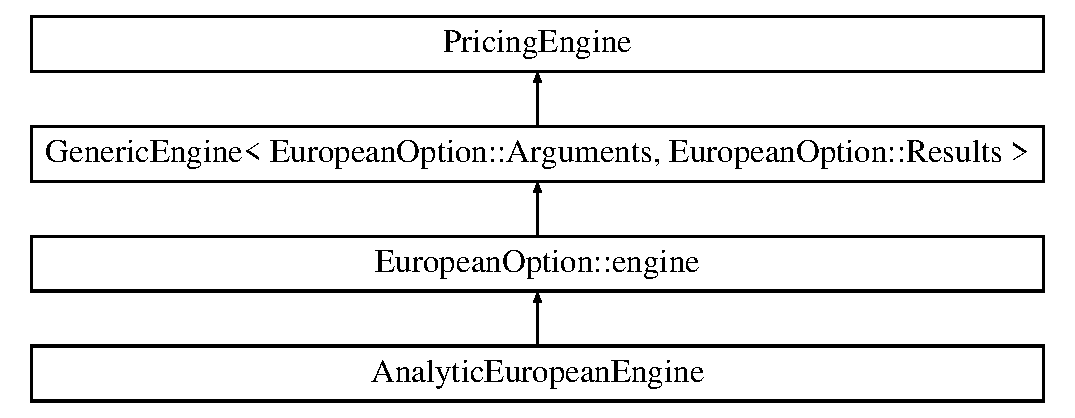
\includegraphics[height=4.000000cm]{class_analytic_european_engine}
\end{center}
\end{figure}
\subsection*{Public Member Functions}
\begin{DoxyCompactItemize}
\item 
\hyperlink{class_analytic_european_engine_ae29c59f14976eaa910d4773d11aa234f}{Analytic\+European\+Engine} (std\+::shared\+\_\+ptr$<$ \hyperlink{class_b_s_stochastic_process}{B\+S\+Stochastic\+Process} $>$ process)
\item 
void \hyperlink{class_analytic_european_engine_adeda22c7b482779d7deaa17037195487}{calculate} () override
\end{DoxyCompactItemize}
\subsection*{Private Attributes}
\begin{DoxyCompactItemize}
\item 
std\+::shared\+\_\+ptr$<$ \hyperlink{class_b_s_stochastic_process}{B\+S\+Stochastic\+Process} $>$ \hyperlink{class_analytic_european_engine_ae9464c6b8aa8b9321b37a8e18b9c785a}{process\+\_\+}
\end{DoxyCompactItemize}
\subsection*{Additional Inherited Members}


\subsection{Constructor \& Destructor Documentation}
\hypertarget{class_analytic_european_engine_ae29c59f14976eaa910d4773d11aa234f}{}\label{class_analytic_european_engine_ae29c59f14976eaa910d4773d11aa234f} 
\index{Analytic\+European\+Engine@{Analytic\+European\+Engine}!Analytic\+European\+Engine@{Analytic\+European\+Engine}}
\index{Analytic\+European\+Engine@{Analytic\+European\+Engine}!Analytic\+European\+Engine@{Analytic\+European\+Engine}}
\subsubsection{\texorpdfstring{Analytic\+European\+Engine()}{AnalyticEuropeanEngine()}}
{\footnotesize\ttfamily Analytic\+European\+Engine\+::\+Analytic\+European\+Engine (\begin{DoxyParamCaption}\item[{std\+::shared\+\_\+ptr$<$ \hyperlink{class_b_s_stochastic_process}{B\+S\+Stochastic\+Process} $>$}]{process }\end{DoxyParamCaption})}



\subsection{Member Function Documentation}
\hypertarget{class_analytic_european_engine_adeda22c7b482779d7deaa17037195487}{}\label{class_analytic_european_engine_adeda22c7b482779d7deaa17037195487} 
\index{Analytic\+European\+Engine@{Analytic\+European\+Engine}!calculate@{calculate}}
\index{calculate@{calculate}!Analytic\+European\+Engine@{Analytic\+European\+Engine}}
\subsubsection{\texorpdfstring{calculate()}{calculate()}}
{\footnotesize\ttfamily void Analytic\+European\+Engine\+::calculate (\begin{DoxyParamCaption}{ }\end{DoxyParamCaption})\hspace{0.3cm}{\ttfamily [override]}, {\ttfamily [virtual]}}



Implements \hyperlink{class_pricing_engine_a733511ffc3cf5e4dc1fbc2a39208d8bd}{Pricing\+Engine}.



\subsection{Member Data Documentation}
\hypertarget{class_analytic_european_engine_ae9464c6b8aa8b9321b37a8e18b9c785a}{}\label{class_analytic_european_engine_ae9464c6b8aa8b9321b37a8e18b9c785a} 
\index{Analytic\+European\+Engine@{Analytic\+European\+Engine}!process\+\_\+@{process\+\_\+}}
\index{process\+\_\+@{process\+\_\+}!Analytic\+European\+Engine@{Analytic\+European\+Engine}}
\subsubsection{\texorpdfstring{process\+\_\+}{process\_}}
{\footnotesize\ttfamily std\+::shared\+\_\+ptr$<$\hyperlink{class_b_s_stochastic_process}{B\+S\+Stochastic\+Process}$>$ Analytic\+European\+Engine\+::process\+\_\+\hspace{0.3cm}{\ttfamily [private]}}



The documentation for this class was generated from the following files\+:\begin{DoxyCompactItemize}
\item 
Users/\+C\+U\+I/\+Dropbox/\+C++/\+Finance/\+Pricing\+Engines/\hyperlink{_analytic_european_engine_8h}{Analytic\+European\+Engine.\+h}\item 
Users/\+C\+U\+I/\+Dropbox/\+C++/\+Finance/\+Pricing\+Engines/\hyperlink{_analytic_european_engine_8cpp}{Analytic\+European\+Engine.\+cpp}\end{DoxyCompactItemize}

\hypertarget{class_analytic_forward_engine}{}\section{Analytic\+Forward\+Engine Class Reference}
\label{class_analytic_forward_engine}\index{Analytic\+Forward\+Engine@{Analytic\+Forward\+Engine}}


{\ttfamily \#include $<$Analytic\+Forward\+Engine.\+h$>$}

Inheritance diagram for Analytic\+Forward\+Engine\+:\begin{figure}[H]
\begin{center}
\leavevmode
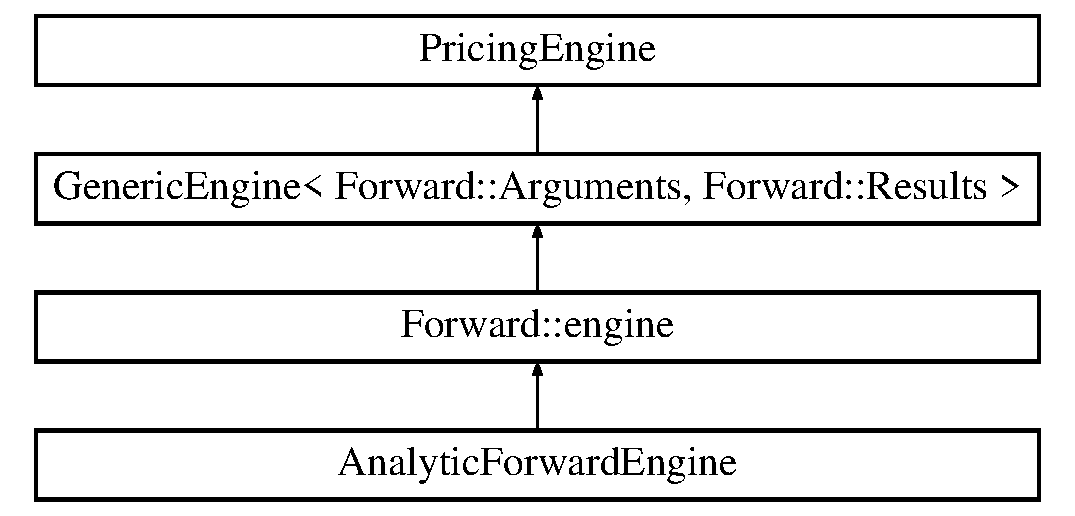
\includegraphics[height=4.000000cm]{class_analytic_forward_engine}
\end{center}
\end{figure}
\subsection*{Public Member Functions}
\begin{DoxyCompactItemize}
\item 
\hyperlink{class_analytic_forward_engine_a7745431773dc2910c8aa01183b7780d0}{Analytic\+Forward\+Engine} (\hyperlink{_name_def_8h_a25bee43a162de339c81f3d1caf6b887d}{Rate} \hyperlink{_uniform_l_ecuyer_r_n_g1_8cpp_a372556d73d7e403d9b677b89b21ee572}{r})
\item 
void \hyperlink{class_analytic_forward_engine_a12d6791a13bf727d43ffcff9cb55b094}{calculate} () override
\end{DoxyCompactItemize}
\subsection*{Private Attributes}
\begin{DoxyCompactItemize}
\item 
\hyperlink{_name_def_8h_a25bee43a162de339c81f3d1caf6b887d}{Rate} \hyperlink{class_analytic_forward_engine_a4398f98b358ec1800db1e8e609b45321}{r\+\_\+}
\end{DoxyCompactItemize}
\subsection*{Additional Inherited Members}


\subsection{Constructor \& Destructor Documentation}
\hypertarget{class_analytic_forward_engine_a7745431773dc2910c8aa01183b7780d0}{}\label{class_analytic_forward_engine_a7745431773dc2910c8aa01183b7780d0} 
\index{Analytic\+Forward\+Engine@{Analytic\+Forward\+Engine}!Analytic\+Forward\+Engine@{Analytic\+Forward\+Engine}}
\index{Analytic\+Forward\+Engine@{Analytic\+Forward\+Engine}!Analytic\+Forward\+Engine@{Analytic\+Forward\+Engine}}
\subsubsection{\texorpdfstring{Analytic\+Forward\+Engine()}{AnalyticForwardEngine()}}
{\footnotesize\ttfamily Analytic\+Forward\+Engine\+::\+Analytic\+Forward\+Engine (\begin{DoxyParamCaption}\item[{\hyperlink{_name_def_8h_a25bee43a162de339c81f3d1caf6b887d}{Rate}}]{r }\end{DoxyParamCaption})}



\subsection{Member Function Documentation}
\hypertarget{class_analytic_forward_engine_a12d6791a13bf727d43ffcff9cb55b094}{}\label{class_analytic_forward_engine_a12d6791a13bf727d43ffcff9cb55b094} 
\index{Analytic\+Forward\+Engine@{Analytic\+Forward\+Engine}!calculate@{calculate}}
\index{calculate@{calculate}!Analytic\+Forward\+Engine@{Analytic\+Forward\+Engine}}
\subsubsection{\texorpdfstring{calculate()}{calculate()}}
{\footnotesize\ttfamily void Analytic\+Forward\+Engine\+::calculate (\begin{DoxyParamCaption}{ }\end{DoxyParamCaption})\hspace{0.3cm}{\ttfamily [override]}, {\ttfamily [virtual]}}



Implements \hyperlink{class_pricing_engine_a733511ffc3cf5e4dc1fbc2a39208d8bd}{Pricing\+Engine}.



\subsection{Member Data Documentation}
\hypertarget{class_analytic_forward_engine_a4398f98b358ec1800db1e8e609b45321}{}\label{class_analytic_forward_engine_a4398f98b358ec1800db1e8e609b45321} 
\index{Analytic\+Forward\+Engine@{Analytic\+Forward\+Engine}!r\+\_\+@{r\+\_\+}}
\index{r\+\_\+@{r\+\_\+}!Analytic\+Forward\+Engine@{Analytic\+Forward\+Engine}}
\subsubsection{\texorpdfstring{r\+\_\+}{r\_}}
{\footnotesize\ttfamily \hyperlink{_name_def_8h_a25bee43a162de339c81f3d1caf6b887d}{Rate} Analytic\+Forward\+Engine\+::r\+\_\+\hspace{0.3cm}{\ttfamily [private]}}



The documentation for this class was generated from the following files\+:\begin{DoxyCompactItemize}
\item 
Users/\+C\+U\+I/\+Dropbox/\+C++/\+Finance/\+Pricing\+Engines/\hyperlink{_analytic_forward_engine_8h}{Analytic\+Forward\+Engine.\+h}\item 
Users/\+C\+U\+I/\+Dropbox/\+C++/\+Finance/\+Pricing\+Engines/\hyperlink{_analytic_forward_engine_8cpp}{Analytic\+Forward\+Engine.\+cpp}\end{DoxyCompactItemize}

\hypertarget{class_antithetic_path}{}\section{Antithetic\+Path Class Reference}
\label{class_antithetic_path}\index{Antithetic\+Path@{Antithetic\+Path}}


{\ttfamily \#include $<$Path.\+h$>$}

Inheritance diagram for Antithetic\+Path\+:\begin{figure}[H]
\begin{center}
\leavevmode
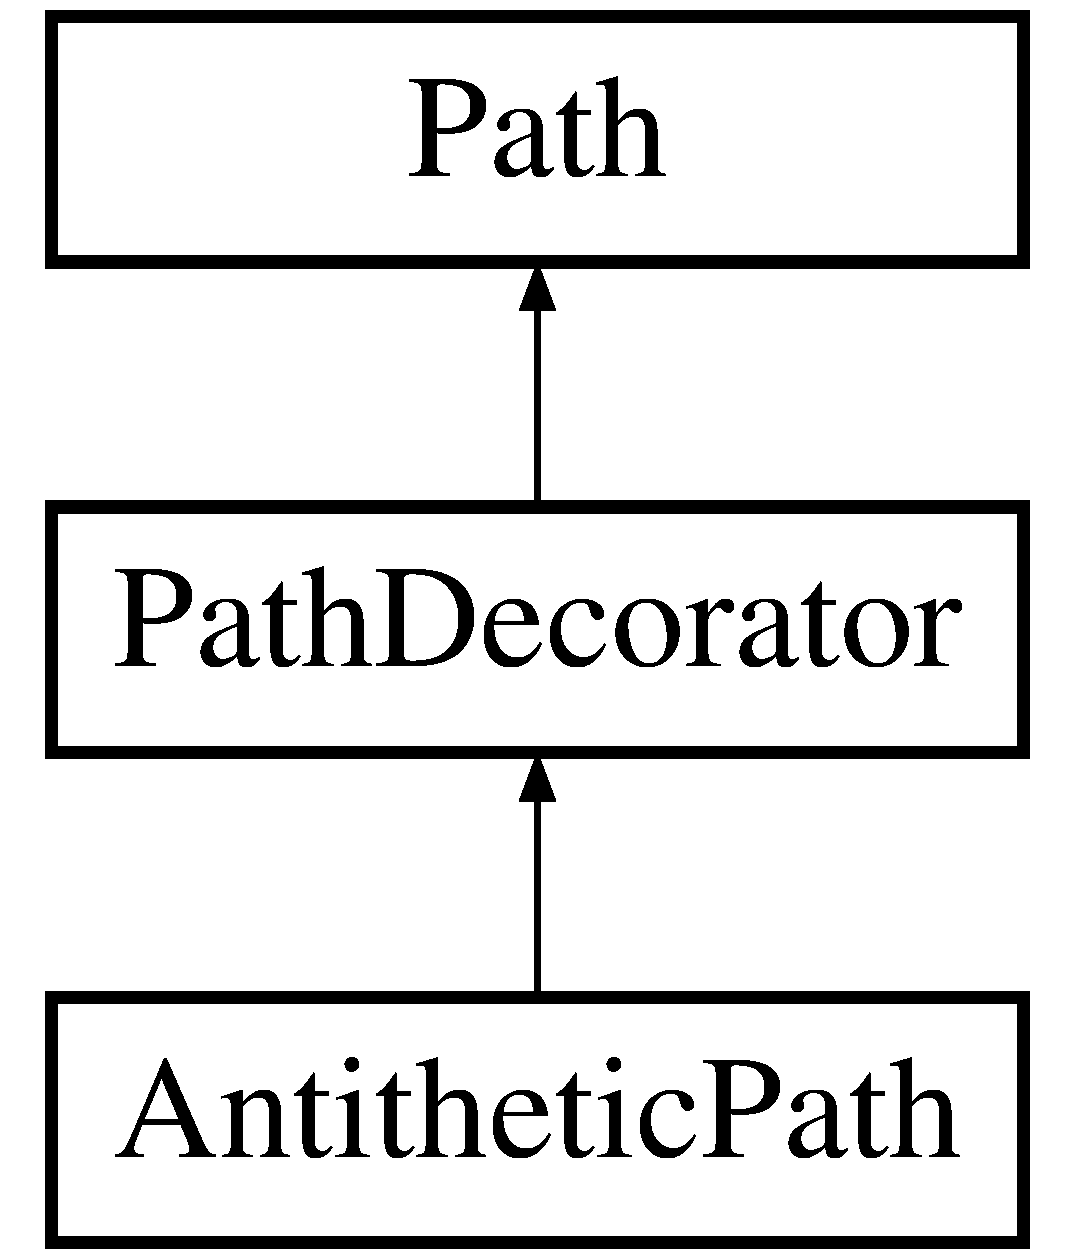
\includegraphics[height=3.000000cm]{class_antithetic_path}
\end{center}
\end{figure}
\subsection*{Public Member Functions}
\begin{DoxyCompactItemize}
\item 
\hyperlink{class_antithetic_path_a3064f50d9c097f15a0472c94871911cc}{Antithetic\+Path} (const vector$<$ \hyperlink{_name_def_8h_ac2d3e0ba793497bcca555c7c2cf64ff3}{Time} $>$ \&time\+Grid, unsigned long dimensional)
\item 
vector$<$ vector$<$ \hyperlink{_name_def_8h_a642a6c5fd87319d922637de0e0bb0305}{Quote} $>$ $>$ \& \hyperlink{class_antithetic_path_a7f94c2a66c0d16ebedba930fbca9d859}{get\+Antithetic\+Values} () override
\item 
const vector$<$ vector$<$ \hyperlink{_name_def_8h_a642a6c5fd87319d922637de0e0bb0305}{Quote} $>$ $>$ \& \hyperlink{class_antithetic_path_a7b6c87162d9c4642dda68b4f9af5f653}{get\+Antithetic\+Values} () const override
\item 
vector$<$ vector$<$ \hyperlink{_name_def_8h_a642a6c5fd87319d922637de0e0bb0305}{Quote} $>$ $>$ \& \hyperlink{class_antithetic_path_a631294808de3c75c98563f292464a7da}{get\+Values} () override
\item 
const vector$<$ vector$<$ \hyperlink{_name_def_8h_a642a6c5fd87319d922637de0e0bb0305}{Quote} $>$ $>$ \& \hyperlink{class_antithetic_path_ad15cfc2a074fd27bd3119ddafa24c3bd}{get\+Values} () const override
\item 
const vector$<$ \hyperlink{_name_def_8h_ac2d3e0ba793497bcca555c7c2cf64ff3}{Time} $>$ \& \hyperlink{class_antithetic_path_a8986e32381ea393159a15dc2b1c0b12c}{get\+Time\+Grid} () const override
\end{DoxyCompactItemize}
\subsection*{Private Attributes}
\begin{DoxyCompactItemize}
\item 
vector$<$ vector$<$ \hyperlink{_name_def_8h_a642a6c5fd87319d922637de0e0bb0305}{Quote} $>$ $>$ \hyperlink{class_antithetic_path_a4aae58299bbbd6516c71fc837bcfe3e7}{anti\+Vals\+\_\+}
\end{DoxyCompactItemize}
\subsection*{Additional Inherited Members}


\subsection{Constructor \& Destructor Documentation}
\hypertarget{class_antithetic_path_a3064f50d9c097f15a0472c94871911cc}{}\label{class_antithetic_path_a3064f50d9c097f15a0472c94871911cc} 
\index{Antithetic\+Path@{Antithetic\+Path}!Antithetic\+Path@{Antithetic\+Path}}
\index{Antithetic\+Path@{Antithetic\+Path}!Antithetic\+Path@{Antithetic\+Path}}
\subsubsection{\texorpdfstring{Antithetic\+Path()}{AntitheticPath()}}
{\footnotesize\ttfamily Antithetic\+Path\+::\+Antithetic\+Path (\begin{DoxyParamCaption}\item[{const vector$<$ \hyperlink{_name_def_8h_ac2d3e0ba793497bcca555c7c2cf64ff3}{Time} $>$ \&}]{time\+Grid,  }\item[{unsigned long}]{dimensional }\end{DoxyParamCaption})}



\subsection{Member Function Documentation}
\hypertarget{class_antithetic_path_a7f94c2a66c0d16ebedba930fbca9d859}{}\label{class_antithetic_path_a7f94c2a66c0d16ebedba930fbca9d859} 
\index{Antithetic\+Path@{Antithetic\+Path}!get\+Antithetic\+Values@{get\+Antithetic\+Values}}
\index{get\+Antithetic\+Values@{get\+Antithetic\+Values}!Antithetic\+Path@{Antithetic\+Path}}
\subsubsection{\texorpdfstring{get\+Antithetic\+Values()}{getAntitheticValues()}\hspace{0.1cm}{\footnotesize\ttfamily [1/2]}}
{\footnotesize\ttfamily vector$<$ vector$<$ \hyperlink{_name_def_8h_a642a6c5fd87319d922637de0e0bb0305}{Quote} $>$ $>$ \& Antithetic\+Path\+::get\+Antithetic\+Values (\begin{DoxyParamCaption}{ }\end{DoxyParamCaption})\hspace{0.3cm}{\ttfamily [override]}, {\ttfamily [virtual]}}



Reimplemented from \hyperlink{class_path_ae6097f4761ac45d2d3656c35f09563f0}{Path}.

\hypertarget{class_antithetic_path_a7b6c87162d9c4642dda68b4f9af5f653}{}\label{class_antithetic_path_a7b6c87162d9c4642dda68b4f9af5f653} 
\index{Antithetic\+Path@{Antithetic\+Path}!get\+Antithetic\+Values@{get\+Antithetic\+Values}}
\index{get\+Antithetic\+Values@{get\+Antithetic\+Values}!Antithetic\+Path@{Antithetic\+Path}}
\subsubsection{\texorpdfstring{get\+Antithetic\+Values()}{getAntitheticValues()}\hspace{0.1cm}{\footnotesize\ttfamily [2/2]}}
{\footnotesize\ttfamily const vector$<$ vector$<$ \hyperlink{_name_def_8h_a642a6c5fd87319d922637de0e0bb0305}{Quote} $>$ $>$ \& Antithetic\+Path\+::get\+Antithetic\+Values (\begin{DoxyParamCaption}{ }\end{DoxyParamCaption}) const\hspace{0.3cm}{\ttfamily [override]}, {\ttfamily [virtual]}}



Reimplemented from \hyperlink{class_path_aadadd7f7ad38c779e36f3ef2805f30e9}{Path}.

\hypertarget{class_antithetic_path_a8986e32381ea393159a15dc2b1c0b12c}{}\label{class_antithetic_path_a8986e32381ea393159a15dc2b1c0b12c} 
\index{Antithetic\+Path@{Antithetic\+Path}!get\+Time\+Grid@{get\+Time\+Grid}}
\index{get\+Time\+Grid@{get\+Time\+Grid}!Antithetic\+Path@{Antithetic\+Path}}
\subsubsection{\texorpdfstring{get\+Time\+Grid()}{getTimeGrid()}}
{\footnotesize\ttfamily const vector$<$ \hyperlink{_name_def_8h_ac2d3e0ba793497bcca555c7c2cf64ff3}{Time} $>$ \& Antithetic\+Path\+::get\+Time\+Grid (\begin{DoxyParamCaption}{ }\end{DoxyParamCaption}) const\hspace{0.3cm}{\ttfamily [override]}, {\ttfamily [virtual]}}



Reimplemented from \hyperlink{class_path_a774bc2169ae87142b8165c3934a9deb9}{Path}.

\hypertarget{class_antithetic_path_a631294808de3c75c98563f292464a7da}{}\label{class_antithetic_path_a631294808de3c75c98563f292464a7da} 
\index{Antithetic\+Path@{Antithetic\+Path}!get\+Values@{get\+Values}}
\index{get\+Values@{get\+Values}!Antithetic\+Path@{Antithetic\+Path}}
\subsubsection{\texorpdfstring{get\+Values()}{getValues()}\hspace{0.1cm}{\footnotesize\ttfamily [1/2]}}
{\footnotesize\ttfamily vector$<$ vector$<$ \hyperlink{_name_def_8h_a642a6c5fd87319d922637de0e0bb0305}{Quote} $>$ $>$ \& Antithetic\+Path\+::get\+Values (\begin{DoxyParamCaption}{ }\end{DoxyParamCaption})\hspace{0.3cm}{\ttfamily [override]}, {\ttfamily [virtual]}}



Reimplemented from \hyperlink{class_path_aeeb21dd5019a717cc8a36ddb0f82f427}{Path}.

\hypertarget{class_antithetic_path_ad15cfc2a074fd27bd3119ddafa24c3bd}{}\label{class_antithetic_path_ad15cfc2a074fd27bd3119ddafa24c3bd} 
\index{Antithetic\+Path@{Antithetic\+Path}!get\+Values@{get\+Values}}
\index{get\+Values@{get\+Values}!Antithetic\+Path@{Antithetic\+Path}}
\subsubsection{\texorpdfstring{get\+Values()}{getValues()}\hspace{0.1cm}{\footnotesize\ttfamily [2/2]}}
{\footnotesize\ttfamily const vector$<$ vector$<$ \hyperlink{_name_def_8h_a642a6c5fd87319d922637de0e0bb0305}{Quote} $>$ $>$ \& Antithetic\+Path\+::get\+Values (\begin{DoxyParamCaption}{ }\end{DoxyParamCaption}) const\hspace{0.3cm}{\ttfamily [override]}, {\ttfamily [virtual]}}



Reimplemented from \hyperlink{class_path_a6d3469e98b5da124b51ca8a9cc2caa28}{Path}.



\subsection{Member Data Documentation}
\hypertarget{class_antithetic_path_a4aae58299bbbd6516c71fc837bcfe3e7}{}\label{class_antithetic_path_a4aae58299bbbd6516c71fc837bcfe3e7} 
\index{Antithetic\+Path@{Antithetic\+Path}!anti\+Vals\+\_\+@{anti\+Vals\+\_\+}}
\index{anti\+Vals\+\_\+@{anti\+Vals\+\_\+}!Antithetic\+Path@{Antithetic\+Path}}
\subsubsection{\texorpdfstring{anti\+Vals\+\_\+}{antiVals\_}}
{\footnotesize\ttfamily vector$<$vector$<$\hyperlink{_name_def_8h_a642a6c5fd87319d922637de0e0bb0305}{Quote}$>$ $>$ Antithetic\+Path\+::anti\+Vals\+\_\+\hspace{0.3cm}{\ttfamily [private]}}



The documentation for this class was generated from the following files\+:\begin{DoxyCompactItemize}
\item 
Mc\+Framework/\hyperlink{_path_8h}{Path.\+h}\item 
Mc\+Framework/\hyperlink{_path_8cpp}{Path.\+cpp}\end{DoxyCompactItemize}

\hypertarget{class_forward_1_1_arguments}{}\section{Forward\+:\+:Arguments Class Reference}
\label{class_forward_1_1_arguments}\index{Forward\+::\+Arguments@{Forward\+::\+Arguments}}


{\ttfamily \#include $<$Forward.\+h$>$}

Inheritance diagram for Forward\+:\+:Arguments\+:\begin{figure}[H]
\begin{center}
\leavevmode
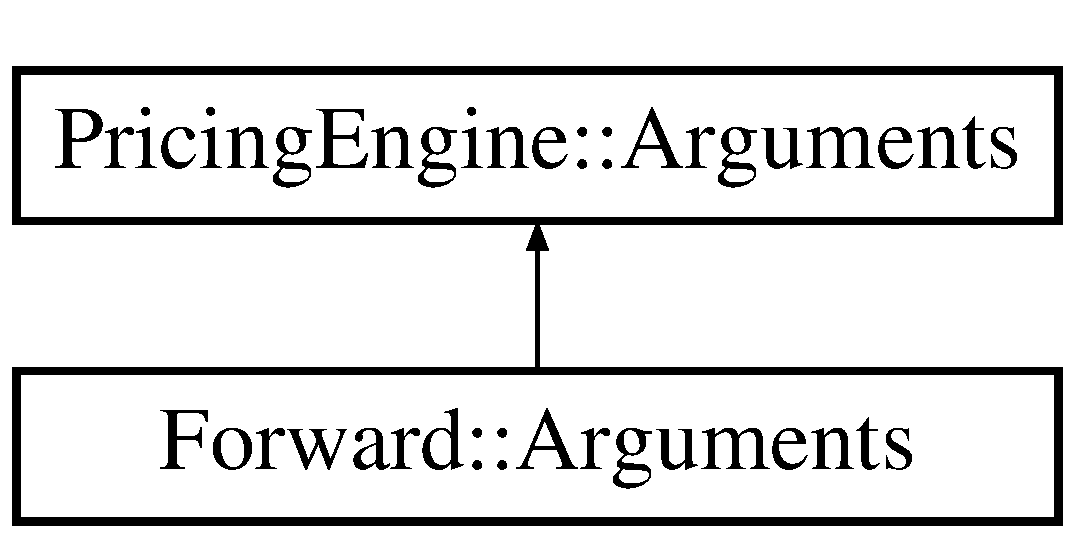
\includegraphics[height=2.000000cm]{class_forward_1_1_arguments}
\end{center}
\end{figure}
\subsection*{Public Attributes}
\begin{DoxyCompactItemize}
\item 
\hyperlink{_name_def_8h_a642a6c5fd87319d922637de0e0bb0305}{Quote} \hyperlink{class_forward_1_1_arguments_acc295ee300d99631259b82448bc1184c}{strike\+\_\+}
\item 
\hyperlink{_name_def_8h_ac2d3e0ba793497bcca555c7c2cf64ff3}{Time} \hyperlink{class_forward_1_1_arguments_abfbb5b4259781ef08e2b48ff4247a484}{maturity\+\_\+}
\item 
\hyperlink{_name_def_8h_a642a6c5fd87319d922637de0e0bb0305}{Quote} \hyperlink{class_forward_1_1_arguments_a407ca35969703b95866bc0c68d49d631}{spot\+\_\+}
\end{DoxyCompactItemize}
\subsection*{Additional Inherited Members}


\subsection{Member Data Documentation}
\hypertarget{class_forward_1_1_arguments_abfbb5b4259781ef08e2b48ff4247a484}{}\label{class_forward_1_1_arguments_abfbb5b4259781ef08e2b48ff4247a484} 
\index{Forward\+::\+Arguments@{Forward\+::\+Arguments}!maturity\+\_\+@{maturity\+\_\+}}
\index{maturity\+\_\+@{maturity\+\_\+}!Forward\+::\+Arguments@{Forward\+::\+Arguments}}
\subsubsection{\texorpdfstring{maturity\+\_\+}{maturity\_}}
{\footnotesize\ttfamily \hyperlink{_name_def_8h_ac2d3e0ba793497bcca555c7c2cf64ff3}{Time} Forward\+::\+Arguments\+::maturity\+\_\+}

\hypertarget{class_forward_1_1_arguments_a407ca35969703b95866bc0c68d49d631}{}\label{class_forward_1_1_arguments_a407ca35969703b95866bc0c68d49d631} 
\index{Forward\+::\+Arguments@{Forward\+::\+Arguments}!spot\+\_\+@{spot\+\_\+}}
\index{spot\+\_\+@{spot\+\_\+}!Forward\+::\+Arguments@{Forward\+::\+Arguments}}
\subsubsection{\texorpdfstring{spot\+\_\+}{spot\_}}
{\footnotesize\ttfamily \hyperlink{_name_def_8h_a642a6c5fd87319d922637de0e0bb0305}{Quote} Forward\+::\+Arguments\+::spot\+\_\+}

\hypertarget{class_forward_1_1_arguments_acc295ee300d99631259b82448bc1184c}{}\label{class_forward_1_1_arguments_acc295ee300d99631259b82448bc1184c} 
\index{Forward\+::\+Arguments@{Forward\+::\+Arguments}!strike\+\_\+@{strike\+\_\+}}
\index{strike\+\_\+@{strike\+\_\+}!Forward\+::\+Arguments@{Forward\+::\+Arguments}}
\subsubsection{\texorpdfstring{strike\+\_\+}{strike\_}}
{\footnotesize\ttfamily \hyperlink{_name_def_8h_a642a6c5fd87319d922637de0e0bb0305}{Quote} Forward\+::\+Arguments\+::strike\+\_\+}



The documentation for this class was generated from the following file\+:\begin{DoxyCompactItemize}
\item 
Instruments/\hyperlink{_forward_8h}{Forward.\+h}\end{DoxyCompactItemize}

\hypertarget{class_pricing_engine_1_1_arguments}{}\section{Pricing\+Engine\+:\+:Arguments Class Reference}
\label{class_pricing_engine_1_1_arguments}\index{Pricing\+Engine\+::\+Arguments@{Pricing\+Engine\+::\+Arguments}}


{\ttfamily \#include $<$Pricing\+Engine.\+h$>$}

Inheritance diagram for Pricing\+Engine\+:\+:Arguments\+:\begin{figure}[H]
\begin{center}
\leavevmode
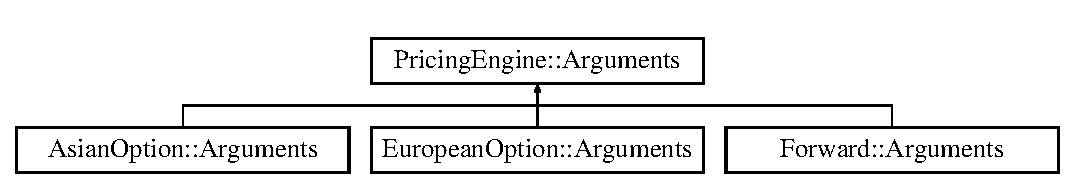
\includegraphics[height=2.000000cm]{class_pricing_engine_1_1_arguments}
\end{center}
\end{figure}
\subsection*{Public Member Functions}
\begin{DoxyCompactItemize}
\item 
\hyperlink{class_pricing_engine_1_1_arguments_a8c28435a8a4be10299e86d62ba72f5f8}{Arguments} ()
\item 
virtual \hyperlink{class_pricing_engine_1_1_arguments_a383465da5f7d0188a540264692ac2eff}{$\sim$\+Arguments} ()
\end{DoxyCompactItemize}


\subsection{Constructor \& Destructor Documentation}
\hypertarget{class_pricing_engine_1_1_arguments_a8c28435a8a4be10299e86d62ba72f5f8}{}\label{class_pricing_engine_1_1_arguments_a8c28435a8a4be10299e86d62ba72f5f8} 
\index{Pricing\+Engine\+::\+Arguments@{Pricing\+Engine\+::\+Arguments}!Arguments@{Arguments}}
\index{Arguments@{Arguments}!Pricing\+Engine\+::\+Arguments@{Pricing\+Engine\+::\+Arguments}}
\subsubsection{\texorpdfstring{Arguments()}{Arguments()}}
{\footnotesize\ttfamily Pricing\+Engine\+::\+Arguments\+::\+Arguments (\begin{DoxyParamCaption}{ }\end{DoxyParamCaption})\hspace{0.3cm}{\ttfamily [inline]}}

\hypertarget{class_pricing_engine_1_1_arguments_a383465da5f7d0188a540264692ac2eff}{}\label{class_pricing_engine_1_1_arguments_a383465da5f7d0188a540264692ac2eff} 
\index{Pricing\+Engine\+::\+Arguments@{Pricing\+Engine\+::\+Arguments}!````~Arguments@{$\sim$\+Arguments}}
\index{````~Arguments@{$\sim$\+Arguments}!Pricing\+Engine\+::\+Arguments@{Pricing\+Engine\+::\+Arguments}}
\subsubsection{\texorpdfstring{$\sim$\+Arguments()}{~Arguments()}}
{\footnotesize\ttfamily virtual Pricing\+Engine\+::\+Arguments\+::$\sim$\+Arguments (\begin{DoxyParamCaption}{ }\end{DoxyParamCaption})\hspace{0.3cm}{\ttfamily [inline]}, {\ttfamily [virtual]}}



The documentation for this class was generated from the following file\+:\begin{DoxyCompactItemize}
\item 
\hyperlink{_pricing_engine_8h}{Pricing\+Engine.\+h}\end{DoxyCompactItemize}

\hypertarget{class_asian_option_1_1_arguments}{}\section{Asian\+Option\+:\+:Arguments Class Reference}
\label{class_asian_option_1_1_arguments}\index{Asian\+Option\+::\+Arguments@{Asian\+Option\+::\+Arguments}}


{\ttfamily \#include $<$Asian\+Option.\+h$>$}

Inheritance diagram for Asian\+Option\+:\+:Arguments\+:\begin{figure}[H]
\begin{center}
\leavevmode
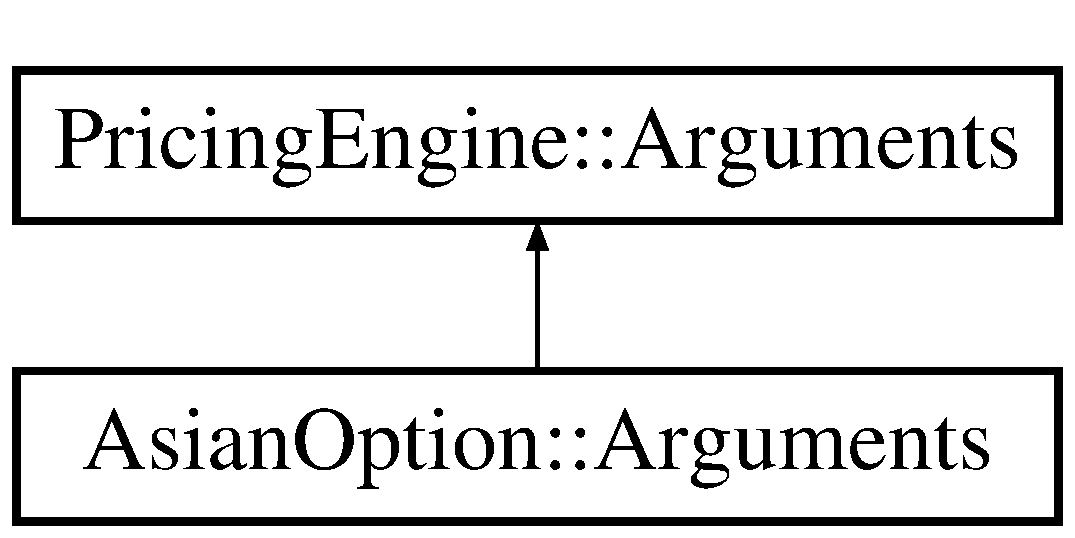
\includegraphics[height=2.000000cm]{class_asian_option_1_1_arguments}
\end{center}
\end{figure}
\subsection*{Public Attributes}
\begin{DoxyCompactItemize}
\item 
std\+::shared\+\_\+ptr$<$ \hyperlink{class_payoff}{Payoff} $>$ \hyperlink{class_asian_option_1_1_arguments_ae44f022e21c05aa688d1d94a0f57d125}{payoff\+\_\+}
\item 
std\+::vector$<$ \hyperlink{_name_def_8h_ac2d3e0ba793497bcca555c7c2cf64ff3}{Time} $>$ \hyperlink{class_asian_option_1_1_arguments_a27e013476613aec57076742ba561a722}{monitored\+Times\+\_\+}
\item 
\hyperlink{_name_def_8h_ac2d3e0ba793497bcca555c7c2cf64ff3}{Time} \hyperlink{class_asian_option_1_1_arguments_ad39a2dee07ec9ec77cb64cb75e44a056}{maturity\+\_\+}
\item 
\hyperlink{class_asian_option_add7292791bf85820ff9fdbfd4407f3b9}{Average\+Type} \hyperlink{class_asian_option_1_1_arguments_aa93577b436b362136035ed3f6fc742bf}{average\+Type\+\_\+}
\end{DoxyCompactItemize}
\subsection*{Additional Inherited Members}


\subsection{Member Data Documentation}
\hypertarget{class_asian_option_1_1_arguments_aa93577b436b362136035ed3f6fc742bf}{}\label{class_asian_option_1_1_arguments_aa93577b436b362136035ed3f6fc742bf} 
\index{Asian\+Option\+::\+Arguments@{Asian\+Option\+::\+Arguments}!average\+Type\+\_\+@{average\+Type\+\_\+}}
\index{average\+Type\+\_\+@{average\+Type\+\_\+}!Asian\+Option\+::\+Arguments@{Asian\+Option\+::\+Arguments}}
\subsubsection{\texorpdfstring{average\+Type\+\_\+}{averageType\_}}
{\footnotesize\ttfamily \hyperlink{class_asian_option_add7292791bf85820ff9fdbfd4407f3b9}{Average\+Type} Asian\+Option\+::\+Arguments\+::average\+Type\+\_\+}

\hypertarget{class_asian_option_1_1_arguments_ad39a2dee07ec9ec77cb64cb75e44a056}{}\label{class_asian_option_1_1_arguments_ad39a2dee07ec9ec77cb64cb75e44a056} 
\index{Asian\+Option\+::\+Arguments@{Asian\+Option\+::\+Arguments}!maturity\+\_\+@{maturity\+\_\+}}
\index{maturity\+\_\+@{maturity\+\_\+}!Asian\+Option\+::\+Arguments@{Asian\+Option\+::\+Arguments}}
\subsubsection{\texorpdfstring{maturity\+\_\+}{maturity\_}}
{\footnotesize\ttfamily \hyperlink{_name_def_8h_ac2d3e0ba793497bcca555c7c2cf64ff3}{Time} Asian\+Option\+::\+Arguments\+::maturity\+\_\+}

\hypertarget{class_asian_option_1_1_arguments_a27e013476613aec57076742ba561a722}{}\label{class_asian_option_1_1_arguments_a27e013476613aec57076742ba561a722} 
\index{Asian\+Option\+::\+Arguments@{Asian\+Option\+::\+Arguments}!monitored\+Times\+\_\+@{monitored\+Times\+\_\+}}
\index{monitored\+Times\+\_\+@{monitored\+Times\+\_\+}!Asian\+Option\+::\+Arguments@{Asian\+Option\+::\+Arguments}}
\subsubsection{\texorpdfstring{monitored\+Times\+\_\+}{monitoredTimes\_}}
{\footnotesize\ttfamily std\+::vector$<$\hyperlink{_name_def_8h_ac2d3e0ba793497bcca555c7c2cf64ff3}{Time}$>$ Asian\+Option\+::\+Arguments\+::monitored\+Times\+\_\+}

\hypertarget{class_asian_option_1_1_arguments_ae44f022e21c05aa688d1d94a0f57d125}{}\label{class_asian_option_1_1_arguments_ae44f022e21c05aa688d1d94a0f57d125} 
\index{Asian\+Option\+::\+Arguments@{Asian\+Option\+::\+Arguments}!payoff\+\_\+@{payoff\+\_\+}}
\index{payoff\+\_\+@{payoff\+\_\+}!Asian\+Option\+::\+Arguments@{Asian\+Option\+::\+Arguments}}
\subsubsection{\texorpdfstring{payoff\+\_\+}{payoff\_}}
{\footnotesize\ttfamily std\+::shared\+\_\+ptr$<$\hyperlink{class_payoff}{Payoff}$>$ Asian\+Option\+::\+Arguments\+::payoff\+\_\+}



The documentation for this class was generated from the following file\+:\begin{DoxyCompactItemize}
\item 
Instruments/\hyperlink{_asian_option_8h}{Asian\+Option.\+h}\end{DoxyCompactItemize}

\hypertarget{class_european_option_1_1_arguments}{}\section{European\+Option\+:\+:Arguments Class Reference}
\label{class_european_option_1_1_arguments}\index{European\+Option\+::\+Arguments@{European\+Option\+::\+Arguments}}


{\ttfamily \#include $<$European\+Option.\+h$>$}

Inheritance diagram for European\+Option\+:\+:Arguments\+:\begin{figure}[H]
\begin{center}
\leavevmode
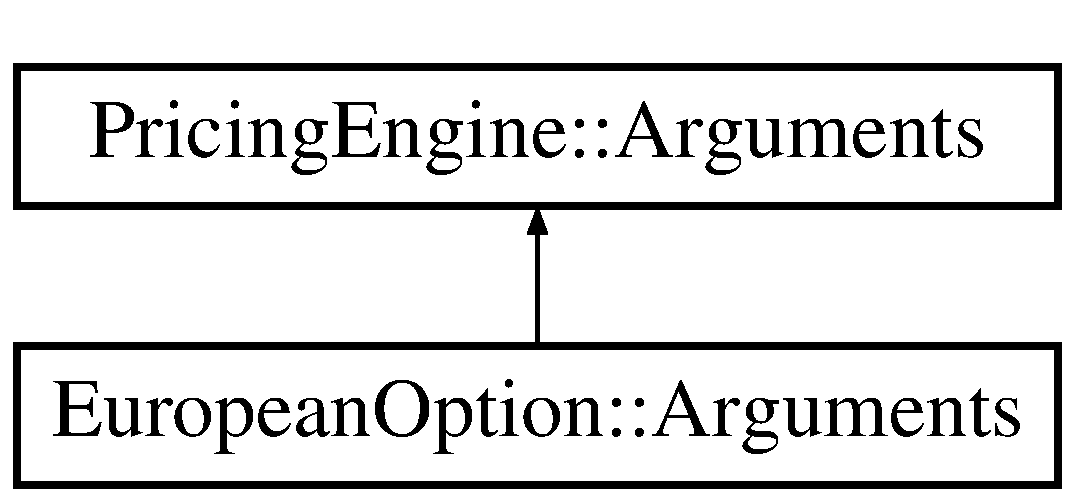
\includegraphics[height=2.000000cm]{class_european_option_1_1_arguments}
\end{center}
\end{figure}
\subsection*{Public Attributes}
\begin{DoxyCompactItemize}
\item 
std\+::shared\+\_\+ptr$<$ \hyperlink{class_payoff}{Payoff} $>$ \hyperlink{class_european_option_1_1_arguments_a01a26c6641a2bb9f439c4191c5eb7d76}{payoff\+\_\+}
\item 
\hyperlink{_name_def_8h_ac2d3e0ba793497bcca555c7c2cf64ff3}{Time} \hyperlink{class_european_option_1_1_arguments_a75cb97c8679f5827e3faa8db031e5196}{maturity\+\_\+}
\end{DoxyCompactItemize}
\subsection*{Additional Inherited Members}


\subsection{Member Data Documentation}
\hypertarget{class_european_option_1_1_arguments_a75cb97c8679f5827e3faa8db031e5196}{}\label{class_european_option_1_1_arguments_a75cb97c8679f5827e3faa8db031e5196} 
\index{European\+Option\+::\+Arguments@{European\+Option\+::\+Arguments}!maturity\+\_\+@{maturity\+\_\+}}
\index{maturity\+\_\+@{maturity\+\_\+}!European\+Option\+::\+Arguments@{European\+Option\+::\+Arguments}}
\subsubsection{\texorpdfstring{maturity\+\_\+}{maturity\_}}
{\footnotesize\ttfamily \hyperlink{_name_def_8h_ac2d3e0ba793497bcca555c7c2cf64ff3}{Time} European\+Option\+::\+Arguments\+::maturity\+\_\+}

\hypertarget{class_european_option_1_1_arguments_a01a26c6641a2bb9f439c4191c5eb7d76}{}\label{class_european_option_1_1_arguments_a01a26c6641a2bb9f439c4191c5eb7d76} 
\index{European\+Option\+::\+Arguments@{European\+Option\+::\+Arguments}!payoff\+\_\+@{payoff\+\_\+}}
\index{payoff\+\_\+@{payoff\+\_\+}!European\+Option\+::\+Arguments@{European\+Option\+::\+Arguments}}
\subsubsection{\texorpdfstring{payoff\+\_\+}{payoff\_}}
{\footnotesize\ttfamily std\+::shared\+\_\+ptr$<$\hyperlink{class_payoff}{Payoff}$>$ European\+Option\+::\+Arguments\+::payoff\+\_\+}



The documentation for this class was generated from the following file\+:\begin{DoxyCompactItemize}
\item 
Instruments/\hyperlink{_european_option_8h}{European\+Option.\+h}\end{DoxyCompactItemize}

\hypertarget{class_asian_option}{}\section{Asian\+Option Class Reference}
\label{class_asian_option}\index{Asian\+Option@{Asian\+Option}}


{\ttfamily \#include $<$Asian\+Option.\+h$>$}

Inheritance diagram for Asian\+Option\+:\begin{figure}[H]
\begin{center}
\leavevmode
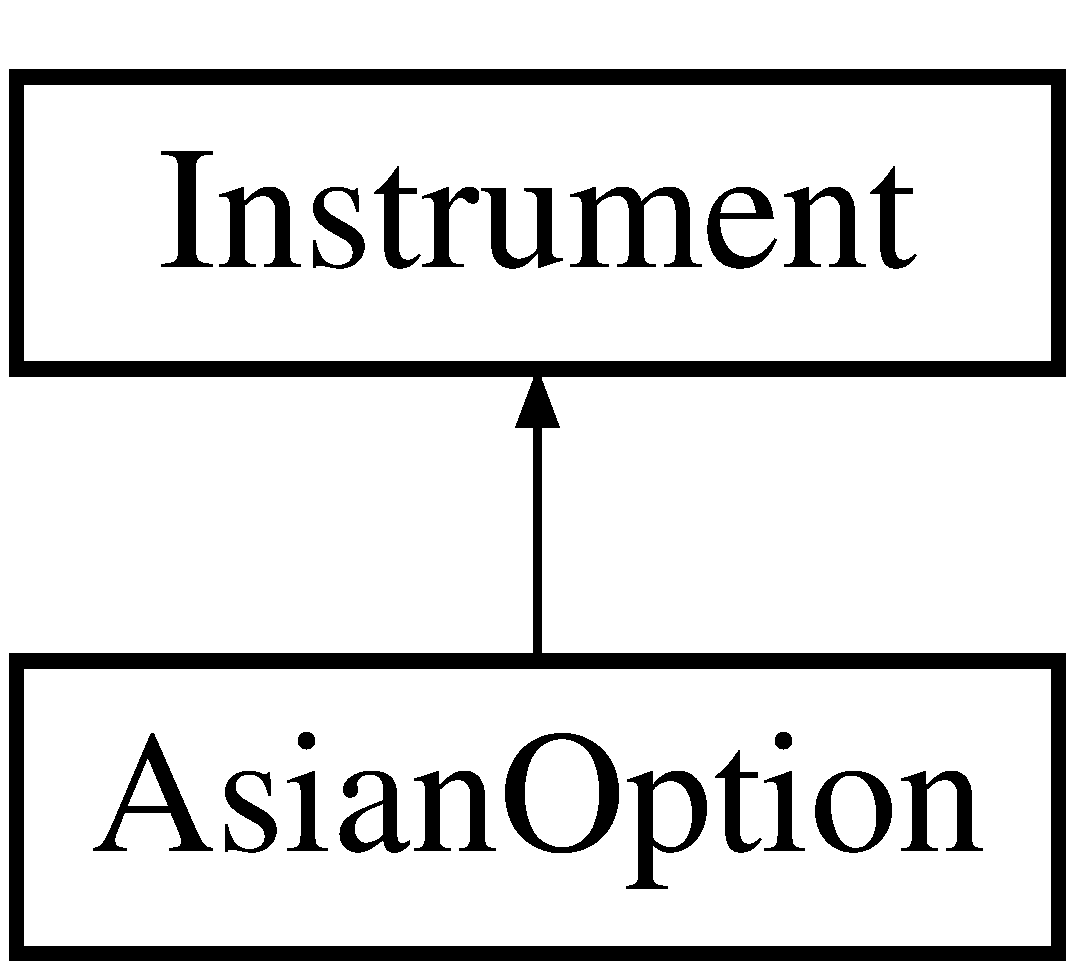
\includegraphics[height=2.000000cm]{class_asian_option}
\end{center}
\end{figure}
\subsection*{Classes}
\begin{DoxyCompactItemize}
\item 
class \hyperlink{class_asian_option_1_1_arguments}{Arguments}
\item 
class \hyperlink{class_asian_option_1_1engine}{engine}
\item 
class \hyperlink{class_asian_option_1_1_results}{Results}
\end{DoxyCompactItemize}
\subsection*{Public Types}
\begin{DoxyCompactItemize}
\item 
enum \hyperlink{class_asian_option_add7292791bf85820ff9fdbfd4407f3b9}{Average\+Type} \{ \hyperlink{class_asian_option_add7292791bf85820ff9fdbfd4407f3b9aff8fffb81d05144807269caa96d3b145}{arithmetic} = 0, 
\hyperlink{class_asian_option_add7292791bf85820ff9fdbfd4407f3b9a17b74dba78a6e25158da4eb685ecfa4e}{geometric} = 1
 \}
\end{DoxyCompactItemize}
\subsection*{Public Member Functions}
\begin{DoxyCompactItemize}
\item 
\hyperlink{class_asian_option_aa4020dfa8edd8d1e8f2756b633b3828b}{Asian\+Option} (\hyperlink{_name_def_8h_ac2d3e0ba793497bcca555c7c2cf64ff3}{Time} maturity, std\+::shared\+\_\+ptr$<$ \hyperlink{class_payoff}{Payoff} $>$ payoff, std\+::vector$<$ \hyperlink{_name_def_8h_ac2d3e0ba793497bcca555c7c2cf64ff3}{Time} $>$ \&monitored\+Times, \hyperlink{class_asian_option_add7292791bf85820ff9fdbfd4407f3b9}{Average\+Type} average\+Type, bool is\+Discretely\+Monitored=1)
\item 
\hyperlink{class_asian_option_a055f90a9d85eac93bac28cc9901489af}{Asian\+Option} (\hyperlink{_name_def_8h_ac2d3e0ba793497bcca555c7c2cf64ff3}{Time} maturity, std\+::shared\+\_\+ptr$<$ \hyperlink{class_payoff}{Payoff} $>$ payoff, \hyperlink{_name_def_8h_ac2d3e0ba793497bcca555c7c2cf64ff3}{Time} time\+Step, \hyperlink{class_asian_option_add7292791bf85820ff9fdbfd4407f3b9}{Average\+Type} average\+Type, bool is\+Discretely\+Monitored=1)
\item 
\hyperlink{class_asian_option_af6dc588a9183209493caf9eb7eb5e572}{Asian\+Option} (\hyperlink{_name_def_8h_ac2d3e0ba793497bcca555c7c2cf64ff3}{Time} maturity, std\+::shared\+\_\+ptr$<$ \hyperlink{class_payoff}{Payoff} $>$ payoff, \hyperlink{class_asian_option_add7292791bf85820ff9fdbfd4407f3b9}{Average\+Type} average\+Type, bool is\+Continuously\+Monitored=1)
\item 
void \hyperlink{class_asian_option_a475cbd83529df369b371ee44f63cdd08}{setup\+Arguments} (\hyperlink{class_pricing_engine_1_1_arguments}{Pricing\+Engine\+::\+Arguments} $\ast$arg) const override
\item 
\hyperlink{_name_def_8h_a5a9d48c16a694e9a2d9f1eca730dc8c5}{Money} \hyperlink{class_asian_option_a99cd9956b73d99a64748c913dcccd6ea}{fetch\+Results} (\hyperlink{class_pricing_engine_1_1_results}{Pricing\+Engine\+::\+Results} $\ast$const res) override
\end{DoxyCompactItemize}
\subsection*{Private Attributes}
\begin{DoxyCompactItemize}
\item 
\hyperlink{_name_def_8h_ac2d3e0ba793497bcca555c7c2cf64ff3}{Time} \hyperlink{class_asian_option_aff2f0be31b55a1b859cde9ee9b339075}{maturity\+\_\+}
\item 
std\+::shared\+\_\+ptr$<$ \hyperlink{class_payoff}{Payoff} $>$ \hyperlink{class_asian_option_abb0ef9b7f812435dcf24e4dd8edb2be2}{payoff\+\_\+}
\item 
std\+::vector$<$ \hyperlink{_name_def_8h_ac2d3e0ba793497bcca555c7c2cf64ff3}{Time} $>$ \hyperlink{class_asian_option_a8cc25f4cabd8ceac95a69598481f18c8}{monitored\+Times\+\_\+}
\item 
std\+::shared\+\_\+ptr$<$ \hyperlink{class_asian_option_1_1_results}{Results} $>$ \hyperlink{class_asian_option_aea29a8aff78cbe4101b4f060cedb6307}{results\+\_\+}
\item 
\hyperlink{class_asian_option_add7292791bf85820ff9fdbfd4407f3b9}{Average\+Type} \hyperlink{class_asian_option_a602d4f41bc033a8242a0641cf5104045}{average\+Type\+\_\+}
\end{DoxyCompactItemize}
\subsection*{Additional Inherited Members}


\subsection{Member Enumeration Documentation}
\hypertarget{class_asian_option_add7292791bf85820ff9fdbfd4407f3b9}{}\label{class_asian_option_add7292791bf85820ff9fdbfd4407f3b9} 
\index{Asian\+Option@{Asian\+Option}!Average\+Type@{Average\+Type}}
\index{Average\+Type@{Average\+Type}!Asian\+Option@{Asian\+Option}}
\subsubsection{\texorpdfstring{Average\+Type}{AverageType}}
{\footnotesize\ttfamily enum \hyperlink{class_asian_option_add7292791bf85820ff9fdbfd4407f3b9}{Asian\+Option\+::\+Average\+Type}}

\begin{DoxyEnumFields}{Enumerator}
\raisebox{\heightof{T}}[0pt][0pt]{\index{arithmetic@{arithmetic}!Asian\+Option@{Asian\+Option}}\index{Asian\+Option@{Asian\+Option}!arithmetic@{arithmetic}}}\hypertarget{class_asian_option_add7292791bf85820ff9fdbfd4407f3b9aff8fffb81d05144807269caa96d3b145}{}\label{class_asian_option_add7292791bf85820ff9fdbfd4407f3b9aff8fffb81d05144807269caa96d3b145} 
arithmetic&\\
\hline

\raisebox{\heightof{T}}[0pt][0pt]{\index{geometric@{geometric}!Asian\+Option@{Asian\+Option}}\index{Asian\+Option@{Asian\+Option}!geometric@{geometric}}}\hypertarget{class_asian_option_add7292791bf85820ff9fdbfd4407f3b9a17b74dba78a6e25158da4eb685ecfa4e}{}\label{class_asian_option_add7292791bf85820ff9fdbfd4407f3b9a17b74dba78a6e25158da4eb685ecfa4e} 
geometric&\\
\hline

\end{DoxyEnumFields}


\subsection{Constructor \& Destructor Documentation}
\hypertarget{class_asian_option_aa4020dfa8edd8d1e8f2756b633b3828b}{}\label{class_asian_option_aa4020dfa8edd8d1e8f2756b633b3828b} 
\index{Asian\+Option@{Asian\+Option}!Asian\+Option@{Asian\+Option}}
\index{Asian\+Option@{Asian\+Option}!Asian\+Option@{Asian\+Option}}
\subsubsection{\texorpdfstring{Asian\+Option()}{AsianOption()}\hspace{0.1cm}{\footnotesize\ttfamily [1/3]}}
{\footnotesize\ttfamily Asian\+Option\+::\+Asian\+Option (\begin{DoxyParamCaption}\item[{\hyperlink{_name_def_8h_ac2d3e0ba793497bcca555c7c2cf64ff3}{Time}}]{maturity,  }\item[{std\+::shared\+\_\+ptr$<$ \hyperlink{class_payoff}{Payoff} $>$}]{payoff,  }\item[{std\+::vector$<$ \hyperlink{_name_def_8h_ac2d3e0ba793497bcca555c7c2cf64ff3}{Time} $>$ \&}]{monitored\+Times,  }\item[{\hyperlink{class_asian_option_add7292791bf85820ff9fdbfd4407f3b9}{Average\+Type}}]{average\+Type,  }\item[{bool}]{is\+Discretely\+Monitored = {\ttfamily 1} }\end{DoxyParamCaption})}

\hypertarget{class_asian_option_a055f90a9d85eac93bac28cc9901489af}{}\label{class_asian_option_a055f90a9d85eac93bac28cc9901489af} 
\index{Asian\+Option@{Asian\+Option}!Asian\+Option@{Asian\+Option}}
\index{Asian\+Option@{Asian\+Option}!Asian\+Option@{Asian\+Option}}
\subsubsection{\texorpdfstring{Asian\+Option()}{AsianOption()}\hspace{0.1cm}{\footnotesize\ttfamily [2/3]}}
{\footnotesize\ttfamily Asian\+Option\+::\+Asian\+Option (\begin{DoxyParamCaption}\item[{\hyperlink{_name_def_8h_ac2d3e0ba793497bcca555c7c2cf64ff3}{Time}}]{maturity,  }\item[{std\+::shared\+\_\+ptr$<$ \hyperlink{class_payoff}{Payoff} $>$}]{payoff,  }\item[{\hyperlink{_name_def_8h_ac2d3e0ba793497bcca555c7c2cf64ff3}{Time}}]{time\+Step,  }\item[{\hyperlink{class_asian_option_add7292791bf85820ff9fdbfd4407f3b9}{Average\+Type}}]{average\+Type,  }\item[{bool}]{is\+Discretely\+Monitored = {\ttfamily 1} }\end{DoxyParamCaption})}

\hypertarget{class_asian_option_af6dc588a9183209493caf9eb7eb5e572}{}\label{class_asian_option_af6dc588a9183209493caf9eb7eb5e572} 
\index{Asian\+Option@{Asian\+Option}!Asian\+Option@{Asian\+Option}}
\index{Asian\+Option@{Asian\+Option}!Asian\+Option@{Asian\+Option}}
\subsubsection{\texorpdfstring{Asian\+Option()}{AsianOption()}\hspace{0.1cm}{\footnotesize\ttfamily [3/3]}}
{\footnotesize\ttfamily Asian\+Option\+::\+Asian\+Option (\begin{DoxyParamCaption}\item[{\hyperlink{_name_def_8h_ac2d3e0ba793497bcca555c7c2cf64ff3}{Time}}]{maturity,  }\item[{std\+::shared\+\_\+ptr$<$ \hyperlink{class_payoff}{Payoff} $>$}]{payoff,  }\item[{\hyperlink{class_asian_option_add7292791bf85820ff9fdbfd4407f3b9}{Average\+Type}}]{average\+Type,  }\item[{bool}]{is\+Continuously\+Monitored = {\ttfamily 1} }\end{DoxyParamCaption})}



\subsection{Member Function Documentation}
\hypertarget{class_asian_option_a99cd9956b73d99a64748c913dcccd6ea}{}\label{class_asian_option_a99cd9956b73d99a64748c913dcccd6ea} 
\index{Asian\+Option@{Asian\+Option}!fetch\+Results@{fetch\+Results}}
\index{fetch\+Results@{fetch\+Results}!Asian\+Option@{Asian\+Option}}
\subsubsection{\texorpdfstring{fetch\+Results()}{fetchResults()}}
{\footnotesize\ttfamily \hyperlink{_name_def_8h_a5a9d48c16a694e9a2d9f1eca730dc8c5}{Money} Asian\+Option\+::fetch\+Results (\begin{DoxyParamCaption}\item[{\hyperlink{class_pricing_engine_1_1_results}{Pricing\+Engine\+::\+Results} $\ast$const}]{res }\end{DoxyParamCaption})\hspace{0.3cm}{\ttfamily [override]}, {\ttfamily [virtual]}}



Implements \hyperlink{class_instrument_a381f093402f789ad7c0ffecd233167dc}{Instrument}.

\hypertarget{class_asian_option_a475cbd83529df369b371ee44f63cdd08}{}\label{class_asian_option_a475cbd83529df369b371ee44f63cdd08} 
\index{Asian\+Option@{Asian\+Option}!setup\+Arguments@{setup\+Arguments}}
\index{setup\+Arguments@{setup\+Arguments}!Asian\+Option@{Asian\+Option}}
\subsubsection{\texorpdfstring{setup\+Arguments()}{setupArguments()}}
{\footnotesize\ttfamily void Asian\+Option\+::setup\+Arguments (\begin{DoxyParamCaption}\item[{\hyperlink{class_pricing_engine_1_1_arguments}{Pricing\+Engine\+::\+Arguments} $\ast$}]{arg }\end{DoxyParamCaption}) const\hspace{0.3cm}{\ttfamily [override]}, {\ttfamily [virtual]}}



Implements \hyperlink{class_instrument_ac0f78fd32a360abde0c31b5bc01c7e67}{Instrument}.



\subsection{Member Data Documentation}
\hypertarget{class_asian_option_a602d4f41bc033a8242a0641cf5104045}{}\label{class_asian_option_a602d4f41bc033a8242a0641cf5104045} 
\index{Asian\+Option@{Asian\+Option}!average\+Type\+\_\+@{average\+Type\+\_\+}}
\index{average\+Type\+\_\+@{average\+Type\+\_\+}!Asian\+Option@{Asian\+Option}}
\subsubsection{\texorpdfstring{average\+Type\+\_\+}{averageType\_}}
{\footnotesize\ttfamily \hyperlink{class_asian_option_add7292791bf85820ff9fdbfd4407f3b9}{Average\+Type} Asian\+Option\+::average\+Type\+\_\+\hspace{0.3cm}{\ttfamily [private]}}

\hypertarget{class_asian_option_aff2f0be31b55a1b859cde9ee9b339075}{}\label{class_asian_option_aff2f0be31b55a1b859cde9ee9b339075} 
\index{Asian\+Option@{Asian\+Option}!maturity\+\_\+@{maturity\+\_\+}}
\index{maturity\+\_\+@{maturity\+\_\+}!Asian\+Option@{Asian\+Option}}
\subsubsection{\texorpdfstring{maturity\+\_\+}{maturity\_}}
{\footnotesize\ttfamily \hyperlink{_name_def_8h_ac2d3e0ba793497bcca555c7c2cf64ff3}{Time} Asian\+Option\+::maturity\+\_\+\hspace{0.3cm}{\ttfamily [private]}}

\hypertarget{class_asian_option_a8cc25f4cabd8ceac95a69598481f18c8}{}\label{class_asian_option_a8cc25f4cabd8ceac95a69598481f18c8} 
\index{Asian\+Option@{Asian\+Option}!monitored\+Times\+\_\+@{monitored\+Times\+\_\+}}
\index{monitored\+Times\+\_\+@{monitored\+Times\+\_\+}!Asian\+Option@{Asian\+Option}}
\subsubsection{\texorpdfstring{monitored\+Times\+\_\+}{monitoredTimes\_}}
{\footnotesize\ttfamily std\+::vector$<$\hyperlink{_name_def_8h_ac2d3e0ba793497bcca555c7c2cf64ff3}{Time}$>$ Asian\+Option\+::monitored\+Times\+\_\+\hspace{0.3cm}{\ttfamily [private]}}

\hypertarget{class_asian_option_abb0ef9b7f812435dcf24e4dd8edb2be2}{}\label{class_asian_option_abb0ef9b7f812435dcf24e4dd8edb2be2} 
\index{Asian\+Option@{Asian\+Option}!payoff\+\_\+@{payoff\+\_\+}}
\index{payoff\+\_\+@{payoff\+\_\+}!Asian\+Option@{Asian\+Option}}
\subsubsection{\texorpdfstring{payoff\+\_\+}{payoff\_}}
{\footnotesize\ttfamily std\+::shared\+\_\+ptr$<$\hyperlink{class_payoff}{Payoff}$>$ Asian\+Option\+::payoff\+\_\+\hspace{0.3cm}{\ttfamily [private]}}

\hypertarget{class_asian_option_aea29a8aff78cbe4101b4f060cedb6307}{}\label{class_asian_option_aea29a8aff78cbe4101b4f060cedb6307} 
\index{Asian\+Option@{Asian\+Option}!results\+\_\+@{results\+\_\+}}
\index{results\+\_\+@{results\+\_\+}!Asian\+Option@{Asian\+Option}}
\subsubsection{\texorpdfstring{results\+\_\+}{results\_}}
{\footnotesize\ttfamily std\+::shared\+\_\+ptr$<$\hyperlink{class_asian_option_1_1_results}{Results}$>$ Asian\+Option\+::results\+\_\+\hspace{0.3cm}{\ttfamily [private]}}



The documentation for this class was generated from the following files\+:\begin{DoxyCompactItemize}
\item 
Users/\+C\+U\+I/\+Dropbox/\+C++/\+Finance/\+Instruments/\hyperlink{_asian_option_8h}{Asian\+Option.\+h}\item 
Users/\+C\+U\+I/\+Dropbox/\+C++/\+Finance/\+Instruments/\hyperlink{_asian_option_8cpp}{Asian\+Option.\+cpp}\end{DoxyCompactItemize}

\hypertarget{class_asian_path_pricer}{}\section{Asian\+Path\+Pricer Class Reference}
\label{class_asian_path_pricer}\index{Asian\+Path\+Pricer@{Asian\+Path\+Pricer}}
Inheritance diagram for Asian\+Path\+Pricer\+:\begin{figure}[H]
\begin{center}
\leavevmode
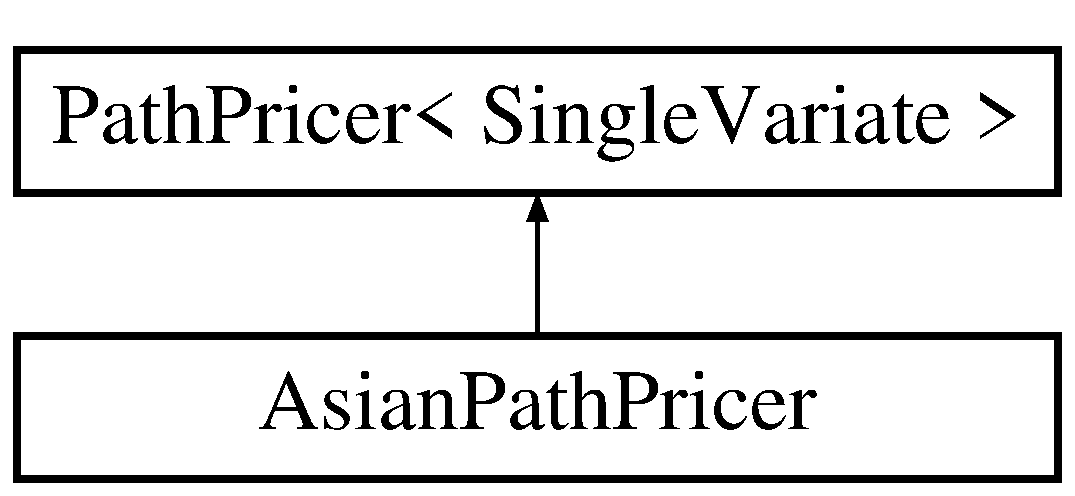
\includegraphics[height=2.000000cm]{class_asian_path_pricer}
\end{center}
\end{figure}
\subsection*{Public Member Functions}
\begin{DoxyCompactItemize}
\item 
\hypertarget{class_asian_path_pricer_a8e295461d8e635e39d8075810bcc1e6a}{}\label{class_asian_path_pricer_a8e295461d8e635e39d8075810bcc1e6a} 
{\bfseries Asian\+Path\+Pricer} (std\+::shared\+\_\+ptr$<$ \hyperlink{class_payoff}{Payoff} $>$ payoff, Rate discount, std\+::shared\+\_\+ptr$<$ vector$<$ Time $>$ $>$ monitored\+Times\+Ptr, Asian\+Option\+::\+Average\+Type average\+Type, bool is\+Antithetic)
\item 
\hypertarget{class_asian_path_pricer_adb10ce912ab34560d762ce0523ae394e}{}\label{class_asian_path_pricer_adb10ce912ab34560d762ce0523ae394e} 
Money {\bfseries operator()} (const \hyperlink{class_path}{Path} \&path) const override
\end{DoxyCompactItemize}


The documentation for this class was generated from the following files\+:\begin{DoxyCompactItemize}
\item 
Users/\+C\+U\+I/\+Dropbox/\+C++/\+Finance/\+Pricing\+Engines/Asian\+Path\+Pricer.\+h\item 
Users/\+C\+U\+I/\+Dropbox/\+C++/\+Finance/\+Pricing\+Engines/Asian\+Path\+Pricer.\+cpp\end{DoxyCompactItemize}

\hypertarget{class_black_scholes_model}{}\section{Black\+Scholes\+Model Class Reference}
\label{class_black_scholes_model}\index{Black\+Scholes\+Model@{Black\+Scholes\+Model}}


{\ttfamily \#include $<$Black\+Scholes\+Model.\+h$>$}

Inheritance diagram for Black\+Scholes\+Model\+:\begin{figure}[H]
\begin{center}
\leavevmode
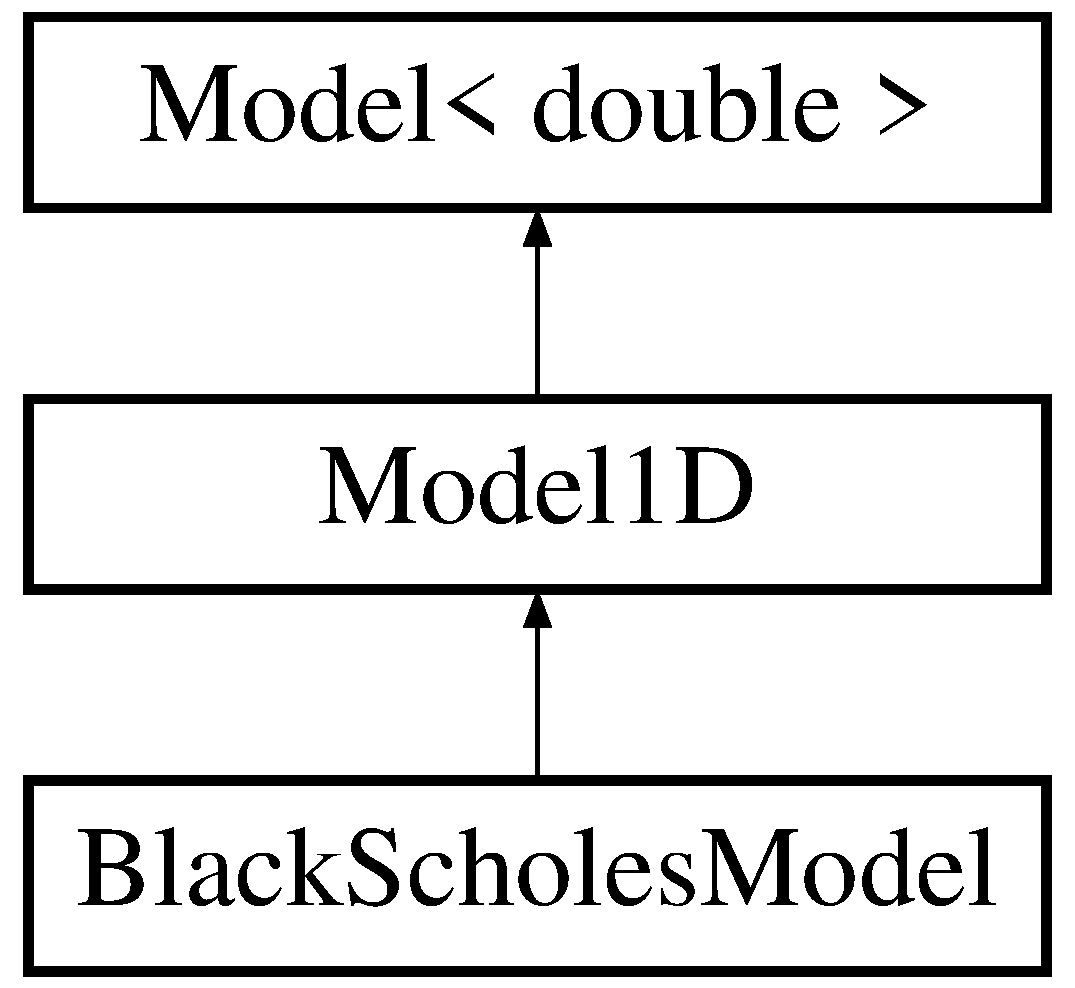
\includegraphics[height=3.000000cm]{class_black_scholes_model}
\end{center}
\end{figure}
\subsection*{Public Member Functions}
\begin{DoxyCompactItemize}
\item 
\hyperlink{class_black_scholes_model_a5cc9ce0cdb0f040da65677b2c07f09b5}{Black\+Scholes\+Model} (std\+::shared\+\_\+ptr$<$ \hyperlink{class_b_s_stochastic_process}{B\+S\+Stochastic\+Process} $>$ process)
\item 
\hyperlink{class_black_scholes_model_a59aa736bd849bc59fed035f702e9813b}{Black\+Scholes\+Model} (double \hyperlink{_uniform_l_ecuyer_r_n_g1_8cpp_a372556d73d7e403d9b677b89b21ee572}{r}, double \hyperlink{_uniform_l_ecuyer_r_n_g1_8cpp_a5cf10165494588b84d4231e0e8a5b1a9}{q}, double sigma, double spot)
\item 
virtual \hyperlink{_name_def_8h_a642a6c5fd87319d922637de0e0bb0305}{Quote} \hyperlink{class_black_scholes_model_a67c3ed604a6d057112ec7e7a1a3fb301}{evolve} (\hyperlink{_name_def_8h_ac2d3e0ba793497bcca555c7c2cf64ff3}{Time} t0, \hyperlink{_name_def_8h_a642a6c5fd87319d922637de0e0bb0305}{Quote} \&x0, \hyperlink{_name_def_8h_ac2d3e0ba793497bcca555c7c2cf64ff3}{Time} dt, double dw) const override
\item 
const vector$<$ int $>$ \& \hyperlink{class_black_scholes_model_a5665e6ea247e4f243082f5c98bbdbad6}{get\+M\+Cdimension} () const override
\item 
void \hyperlink{class_black_scholes_model_a04a6ba4c59cd70a92dedbeb482e9d5aa}{setup\+Argument} (\hyperlink{_name_def_8h_ac2d3e0ba793497bcca555c7c2cf64ff3}{Time} t, \hyperlink{_name_def_8h_ac2d3e0ba793497bcca555c7c2cf64ff3}{Time} dt, \hyperlink{class_generic_random_variable_generator_1_1_argument}{Generic\+Random\+Variable\+Generator\+::\+Argument} $\ast$arg) override
\end{DoxyCompactItemize}
\subsection*{Private Attributes}
\begin{DoxyCompactItemize}
\item 
vector$<$ int $>$ \hyperlink{class_black_scholes_model_a9457c1edc58d9f737f7eeeaaa6812488}{M\+Cdimension\+\_\+}
\end{DoxyCompactItemize}
\subsection*{Additional Inherited Members}


\subsection{Constructor \& Destructor Documentation}
\hypertarget{class_black_scholes_model_a5cc9ce0cdb0f040da65677b2c07f09b5}{}\label{class_black_scholes_model_a5cc9ce0cdb0f040da65677b2c07f09b5} 
\index{Black\+Scholes\+Model@{Black\+Scholes\+Model}!Black\+Scholes\+Model@{Black\+Scholes\+Model}}
\index{Black\+Scholes\+Model@{Black\+Scholes\+Model}!Black\+Scholes\+Model@{Black\+Scholes\+Model}}
\subsubsection{\texorpdfstring{Black\+Scholes\+Model()}{BlackScholesModel()}\hspace{0.1cm}{\footnotesize\ttfamily [1/2]}}
{\footnotesize\ttfamily Black\+Scholes\+Model\+::\+Black\+Scholes\+Model (\begin{DoxyParamCaption}\item[{std\+::shared\+\_\+ptr$<$ \hyperlink{class_b_s_stochastic_process}{B\+S\+Stochastic\+Process} $>$}]{process }\end{DoxyParamCaption})}

\hypertarget{class_black_scholes_model_a59aa736bd849bc59fed035f702e9813b}{}\label{class_black_scholes_model_a59aa736bd849bc59fed035f702e9813b} 
\index{Black\+Scholes\+Model@{Black\+Scholes\+Model}!Black\+Scholes\+Model@{Black\+Scholes\+Model}}
\index{Black\+Scholes\+Model@{Black\+Scholes\+Model}!Black\+Scholes\+Model@{Black\+Scholes\+Model}}
\subsubsection{\texorpdfstring{Black\+Scholes\+Model()}{BlackScholesModel()}\hspace{0.1cm}{\footnotesize\ttfamily [2/2]}}
{\footnotesize\ttfamily Black\+Scholes\+Model\+::\+Black\+Scholes\+Model (\begin{DoxyParamCaption}\item[{double}]{r,  }\item[{double}]{q,  }\item[{double}]{sigma,  }\item[{double}]{spot }\end{DoxyParamCaption})}



\subsection{Member Function Documentation}
\hypertarget{class_black_scholes_model_a67c3ed604a6d057112ec7e7a1a3fb301}{}\label{class_black_scholes_model_a67c3ed604a6d057112ec7e7a1a3fb301} 
\index{Black\+Scholes\+Model@{Black\+Scholes\+Model}!evolve@{evolve}}
\index{evolve@{evolve}!Black\+Scholes\+Model@{Black\+Scholes\+Model}}
\subsubsection{\texorpdfstring{evolve()}{evolve()}}
{\footnotesize\ttfamily \hyperlink{_name_def_8h_a642a6c5fd87319d922637de0e0bb0305}{Quote} Black\+Scholes\+Model\+::evolve (\begin{DoxyParamCaption}\item[{\hyperlink{_name_def_8h_ac2d3e0ba793497bcca555c7c2cf64ff3}{Time}}]{t0,  }\item[{\hyperlink{_name_def_8h_a642a6c5fd87319d922637de0e0bb0305}{Quote} \&}]{x0,  }\item[{\hyperlink{_name_def_8h_ac2d3e0ba793497bcca555c7c2cf64ff3}{Time}}]{dt,  }\item[{double}]{dw }\end{DoxyParamCaption}) const\hspace{0.3cm}{\ttfamily [override]}, {\ttfamily [virtual]}}



Reimplemented from \hyperlink{class_model_a18b1fe1476b5adde8d6125e7f6a7f932}{Model$<$ double $>$}.

\hypertarget{class_black_scholes_model_a5665e6ea247e4f243082f5c98bbdbad6}{}\label{class_black_scholes_model_a5665e6ea247e4f243082f5c98bbdbad6} 
\index{Black\+Scholes\+Model@{Black\+Scholes\+Model}!get\+M\+Cdimension@{get\+M\+Cdimension}}
\index{get\+M\+Cdimension@{get\+M\+Cdimension}!Black\+Scholes\+Model@{Black\+Scholes\+Model}}
\subsubsection{\texorpdfstring{get\+M\+Cdimension()}{getMCdimension()}}
{\footnotesize\ttfamily const vector$<$int$>$\& Black\+Scholes\+Model\+::get\+M\+Cdimension (\begin{DoxyParamCaption}{ }\end{DoxyParamCaption}) const\hspace{0.3cm}{\ttfamily [inline]}, {\ttfamily [override]}, {\ttfamily [virtual]}}



Implements \hyperlink{class_model_a11fb36244c91ca8c36317581b73bca08}{Model$<$ double $>$}.

\hypertarget{class_black_scholes_model_a04a6ba4c59cd70a92dedbeb482e9d5aa}{}\label{class_black_scholes_model_a04a6ba4c59cd70a92dedbeb482e9d5aa} 
\index{Black\+Scholes\+Model@{Black\+Scholes\+Model}!setup\+Argument@{setup\+Argument}}
\index{setup\+Argument@{setup\+Argument}!Black\+Scholes\+Model@{Black\+Scholes\+Model}}
\subsubsection{\texorpdfstring{setup\+Argument()}{setupArgument()}}
{\footnotesize\ttfamily void Black\+Scholes\+Model\+::setup\+Argument (\begin{DoxyParamCaption}\item[{\hyperlink{_name_def_8h_ac2d3e0ba793497bcca555c7c2cf64ff3}{Time}}]{t,  }\item[{\hyperlink{_name_def_8h_ac2d3e0ba793497bcca555c7c2cf64ff3}{Time}}]{dt,  }\item[{\hyperlink{class_generic_random_variable_generator_1_1_argument}{Generic\+Random\+Variable\+Generator\+::\+Argument} $\ast$}]{arg }\end{DoxyParamCaption})\hspace{0.3cm}{\ttfamily [inline]}, {\ttfamily [override]}, {\ttfamily [virtual]}}



Reimplemented from \hyperlink{class_model_a19ba3a18a45aad9012dbc6cbafb09e39}{Model$<$ double $>$}.



\subsection{Member Data Documentation}
\hypertarget{class_black_scholes_model_a9457c1edc58d9f737f7eeeaaa6812488}{}\label{class_black_scholes_model_a9457c1edc58d9f737f7eeeaaa6812488} 
\index{Black\+Scholes\+Model@{Black\+Scholes\+Model}!M\+Cdimension\+\_\+@{M\+Cdimension\+\_\+}}
\index{M\+Cdimension\+\_\+@{M\+Cdimension\+\_\+}!Black\+Scholes\+Model@{Black\+Scholes\+Model}}
\subsubsection{\texorpdfstring{M\+Cdimension\+\_\+}{MCdimension\_}}
{\footnotesize\ttfamily vector$<$int$>$ Black\+Scholes\+Model\+::\+M\+Cdimension\+\_\+\hspace{0.3cm}{\ttfamily [private]}}



The documentation for this class was generated from the following files\+:\begin{DoxyCompactItemize}
\item 
Models/\hyperlink{_black_scholes_model_8h}{Black\+Scholes\+Model.\+h}\item 
Models/\hyperlink{_black_scholes_model_8cpp}{Black\+Scholes\+Model.\+cpp}\end{DoxyCompactItemize}

\hypertarget{class_b_s_stochastic_process}{}\section{B\+S\+Stochastic\+Process Class Reference}
\label{class_b_s_stochastic_process}\index{B\+S\+Stochastic\+Process@{B\+S\+Stochastic\+Process}}


{\ttfamily \#include $<$B\+S\+Stochastic\+Process.\+h$>$}

Inheritance diagram for B\+S\+Stochastic\+Process\+:\begin{figure}[H]
\begin{center}
\leavevmode
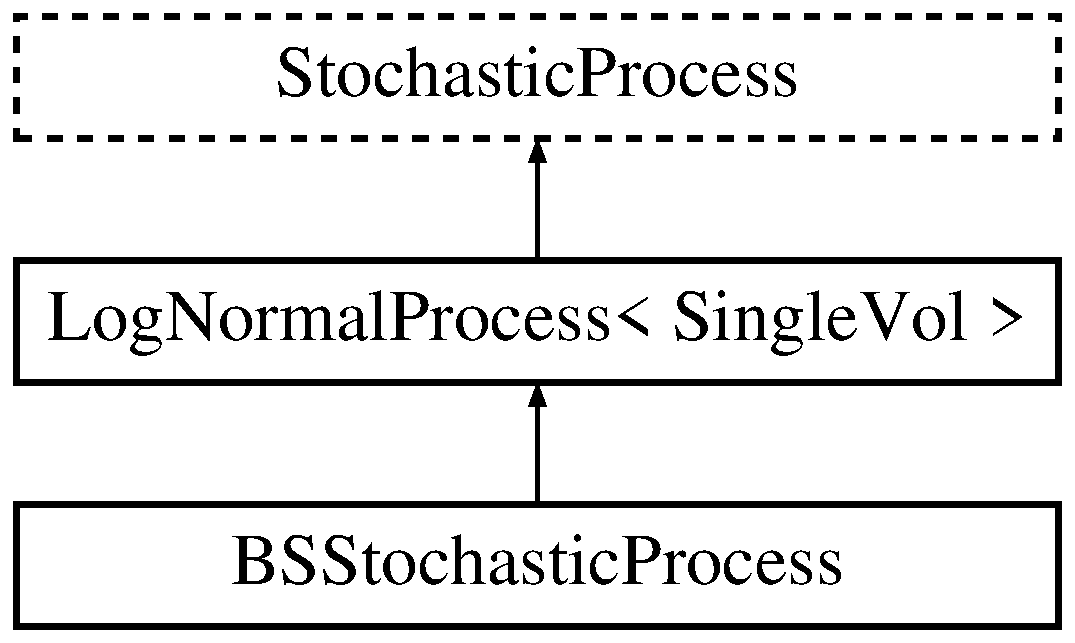
\includegraphics[height=3.000000cm]{class_b_s_stochastic_process}
\end{center}
\end{figure}
\subsection*{Public Member Functions}
\begin{DoxyCompactItemize}
\item 
\hyperlink{class_b_s_stochastic_process_aed9545004ecc3b8a23e95e6406f48327}{B\+S\+Stochastic\+Process} (double \hyperlink{_uniform_l_ecuyer_r_n_g1_8cpp_a372556d73d7e403d9b677b89b21ee572}{r}, double \hyperlink{_uniform_l_ecuyer_r_n_g1_8cpp_a5cf10165494588b84d4231e0e8a5b1a9}{q}, double sigma, double spot)
\item 
\hyperlink{_name_def_8h_a25bee43a162de339c81f3d1caf6b887d}{Rate} \hyperlink{class_b_s_stochastic_process_a9cd46cb3dceb0aee302bf3a6c2ea39a1}{get\+Risk\+Free} () const
\item 
\hyperlink{_name_def_8h_a25bee43a162de339c81f3d1caf6b887d}{Rate} \hyperlink{class_b_s_stochastic_process_a42caffac3e61f92af6849b86df0d9b6b}{get\+Dividend} () const
\item 
\hyperlink{_name_def_8h_a25bee43a162de339c81f3d1caf6b887d}{Rate} \hyperlink{class_b_s_stochastic_process_ab63f363e94441ed0ee22ef10beea16a6}{get\+Volatility} () const
\item 
\hyperlink{_name_def_8h_a25bee43a162de339c81f3d1caf6b887d}{Rate} \hyperlink{class_b_s_stochastic_process_ad20afb9e82ee123452a7d828837289f6}{get\+Volatility} (\hyperlink{_name_def_8h_ac2d3e0ba793497bcca555c7c2cf64ff3}{Time} t) const override
\end{DoxyCompactItemize}
\subsection*{Public Attributes}
\begin{DoxyCompactItemize}
\item 
double \hyperlink{class_b_s_stochastic_process_a9c68fc36f4fceb55eb3b7b812060a391}{r\+\_\+}
\item 
double \hyperlink{class_b_s_stochastic_process_a5f8464c5c964643c947cb5cdc4d6a016}{q\+\_\+}
\item 
double \hyperlink{class_b_s_stochastic_process_aad38cd49eaf86dba80088e6a986a1ca5}{sigma\+\_\+}
\end{DoxyCompactItemize}
\subsection*{Additional Inherited Members}


\subsection{Constructor \& Destructor Documentation}
\hypertarget{class_b_s_stochastic_process_aed9545004ecc3b8a23e95e6406f48327}{}\label{class_b_s_stochastic_process_aed9545004ecc3b8a23e95e6406f48327} 
\index{B\+S\+Stochastic\+Process@{B\+S\+Stochastic\+Process}!B\+S\+Stochastic\+Process@{B\+S\+Stochastic\+Process}}
\index{B\+S\+Stochastic\+Process@{B\+S\+Stochastic\+Process}!B\+S\+Stochastic\+Process@{B\+S\+Stochastic\+Process}}
\subsubsection{\texorpdfstring{B\+S\+Stochastic\+Process()}{BSStochasticProcess()}}
{\footnotesize\ttfamily B\+S\+Stochastic\+Process\+::\+B\+S\+Stochastic\+Process (\begin{DoxyParamCaption}\item[{double}]{r,  }\item[{double}]{q,  }\item[{double}]{sigma,  }\item[{double}]{spot }\end{DoxyParamCaption})}


\begin{DoxyParams}{Parameters}
{\em r} & riskfree rate \\
\hline
{\em q} & dividend rate \\
\hline
{\em sigma} & annualized volatility in percentage \\
\hline
{\em spot} & spot price of the underlying \\
\hline
\end{DoxyParams}


\subsection{Member Function Documentation}
\hypertarget{class_b_s_stochastic_process_a42caffac3e61f92af6849b86df0d9b6b}{}\label{class_b_s_stochastic_process_a42caffac3e61f92af6849b86df0d9b6b} 
\index{B\+S\+Stochastic\+Process@{B\+S\+Stochastic\+Process}!get\+Dividend@{get\+Dividend}}
\index{get\+Dividend@{get\+Dividend}!B\+S\+Stochastic\+Process@{B\+S\+Stochastic\+Process}}
\subsubsection{\texorpdfstring{get\+Dividend()}{getDividend()}}
{\footnotesize\ttfamily double B\+S\+Stochastic\+Process\+::get\+Dividend (\begin{DoxyParamCaption}{ }\end{DoxyParamCaption}) const}

\hypertarget{class_b_s_stochastic_process_a9cd46cb3dceb0aee302bf3a6c2ea39a1}{}\label{class_b_s_stochastic_process_a9cd46cb3dceb0aee302bf3a6c2ea39a1} 
\index{B\+S\+Stochastic\+Process@{B\+S\+Stochastic\+Process}!get\+Risk\+Free@{get\+Risk\+Free}}
\index{get\+Risk\+Free@{get\+Risk\+Free}!B\+S\+Stochastic\+Process@{B\+S\+Stochastic\+Process}}
\subsubsection{\texorpdfstring{get\+Risk\+Free()}{getRiskFree()}}
{\footnotesize\ttfamily double B\+S\+Stochastic\+Process\+::get\+Risk\+Free (\begin{DoxyParamCaption}{ }\end{DoxyParamCaption}) const}

\hypertarget{class_b_s_stochastic_process_ab63f363e94441ed0ee22ef10beea16a6}{}\label{class_b_s_stochastic_process_ab63f363e94441ed0ee22ef10beea16a6} 
\index{B\+S\+Stochastic\+Process@{B\+S\+Stochastic\+Process}!get\+Volatility@{get\+Volatility}}
\index{get\+Volatility@{get\+Volatility}!B\+S\+Stochastic\+Process@{B\+S\+Stochastic\+Process}}
\subsubsection{\texorpdfstring{get\+Volatility()}{getVolatility()}\hspace{0.1cm}{\footnotesize\ttfamily [1/2]}}
{\footnotesize\ttfamily double B\+S\+Stochastic\+Process\+::get\+Volatility (\begin{DoxyParamCaption}{ }\end{DoxyParamCaption}) const}

\hypertarget{class_b_s_stochastic_process_ad20afb9e82ee123452a7d828837289f6}{}\label{class_b_s_stochastic_process_ad20afb9e82ee123452a7d828837289f6} 
\index{B\+S\+Stochastic\+Process@{B\+S\+Stochastic\+Process}!get\+Volatility@{get\+Volatility}}
\index{get\+Volatility@{get\+Volatility}!B\+S\+Stochastic\+Process@{B\+S\+Stochastic\+Process}}
\subsubsection{\texorpdfstring{get\+Volatility()}{getVolatility()}\hspace{0.1cm}{\footnotesize\ttfamily [2/2]}}
{\footnotesize\ttfamily \hyperlink{_name_def_8h_a25bee43a162de339c81f3d1caf6b887d}{Rate} B\+S\+Stochastic\+Process\+::get\+Volatility (\begin{DoxyParamCaption}\item[{\hyperlink{_name_def_8h_ac2d3e0ba793497bcca555c7c2cf64ff3}{Time}}]{t }\end{DoxyParamCaption}) const\hspace{0.3cm}{\ttfamily [inline]}, {\ttfamily [override]}, {\ttfamily [virtual]}}



Reimplemented from \hyperlink{class_log_normal_process_af2d153f75cd5efbeaa3a9028585dd835}{Log\+Normal\+Process$<$ Single\+Vol $>$}.



\subsection{Member Data Documentation}
\hypertarget{class_b_s_stochastic_process_a5f8464c5c964643c947cb5cdc4d6a016}{}\label{class_b_s_stochastic_process_a5f8464c5c964643c947cb5cdc4d6a016} 
\index{B\+S\+Stochastic\+Process@{B\+S\+Stochastic\+Process}!q\+\_\+@{q\+\_\+}}
\index{q\+\_\+@{q\+\_\+}!B\+S\+Stochastic\+Process@{B\+S\+Stochastic\+Process}}
\subsubsection{\texorpdfstring{q\+\_\+}{q\_}}
{\footnotesize\ttfamily double B\+S\+Stochastic\+Process\+::q\+\_\+}

\hypertarget{class_b_s_stochastic_process_a9c68fc36f4fceb55eb3b7b812060a391}{}\label{class_b_s_stochastic_process_a9c68fc36f4fceb55eb3b7b812060a391} 
\index{B\+S\+Stochastic\+Process@{B\+S\+Stochastic\+Process}!r\+\_\+@{r\+\_\+}}
\index{r\+\_\+@{r\+\_\+}!B\+S\+Stochastic\+Process@{B\+S\+Stochastic\+Process}}
\subsubsection{\texorpdfstring{r\+\_\+}{r\_}}
{\footnotesize\ttfamily double B\+S\+Stochastic\+Process\+::r\+\_\+}

\hypertarget{class_b_s_stochastic_process_aad38cd49eaf86dba80088e6a986a1ca5}{}\label{class_b_s_stochastic_process_aad38cd49eaf86dba80088e6a986a1ca5} 
\index{B\+S\+Stochastic\+Process@{B\+S\+Stochastic\+Process}!sigma\+\_\+@{sigma\+\_\+}}
\index{sigma\+\_\+@{sigma\+\_\+}!B\+S\+Stochastic\+Process@{B\+S\+Stochastic\+Process}}
\subsubsection{\texorpdfstring{sigma\+\_\+}{sigma\_}}
{\footnotesize\ttfamily double B\+S\+Stochastic\+Process\+::sigma\+\_\+}



The documentation for this class was generated from the following files\+:\begin{DoxyCompactItemize}
\item 
Stochastic\+Processes/\hyperlink{_b_s_stochastic_process_8h}{B\+S\+Stochastic\+Process.\+h}\item 
Stochastic\+Processes/\hyperlink{_b_s_stochastic_process_8cpp}{B\+S\+Stochastic\+Process.\+cpp}\end{DoxyCompactItemize}

\hypertarget{class_constant_parameter}{}\section{Constant\+Parameter Class Reference}
\label{class_constant_parameter}\index{Constant\+Parameter@{Constant\+Parameter}}
Inheritance diagram for Constant\+Parameter\+:\begin{figure}[H]
\begin{center}
\leavevmode
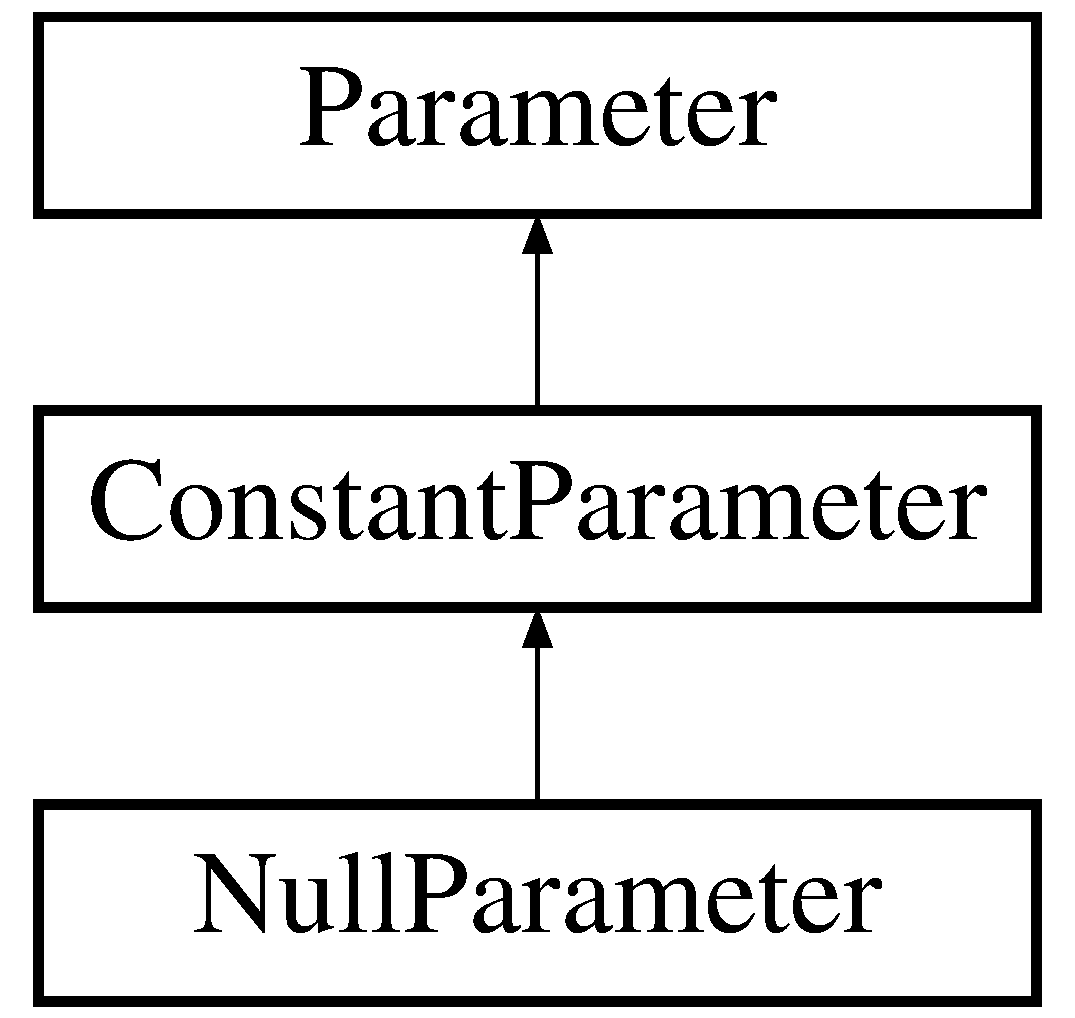
\includegraphics[height=3.000000cm]{class_constant_parameter}
\end{center}
\end{figure}
\subsection*{Public Member Functions}
\begin{DoxyCompactItemize}
\item 
\hypertarget{class_constant_parameter_ae3bc9ec65c93b6b88fe04dcb7010d897}{}\label{class_constant_parameter_ae3bc9ec65c93b6b88fe04dcb7010d897} 
{\bfseries Constant\+Parameter} (double param)
\item 
\hypertarget{class_constant_parameter_a23abb141692843e2ef68d43f610beb5e}{}\label{class_constant_parameter_a23abb141692843e2ef68d43f610beb5e} 
double {\bfseries operator()} (Time t) const override
\end{DoxyCompactItemize}
\subsection*{Additional Inherited Members}


The documentation for this class was generated from the following files\+:\begin{DoxyCompactItemize}
\item 
Users/\+C\+U\+I/\+Dropbox/\+C++/\+Finance/Parameter.\+h\item 
Users/\+C\+U\+I/\+Dropbox/\+C++/\+Finance/Parameter.\+cpp\end{DoxyCompactItemize}

\hypertarget{class_european_option_1_1engine}{}\section{European\+Option\+:\+:engine Class Reference}
\label{class_european_option_1_1engine}\index{European\+Option\+::engine@{European\+Option\+::engine}}


{\ttfamily \#include $<$European\+Option.\+h$>$}

Inheritance diagram for European\+Option\+:\+:engine\+:\begin{figure}[H]
\begin{center}
\leavevmode
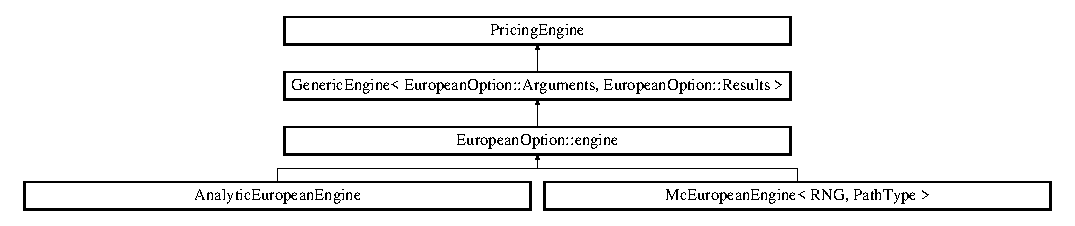
\includegraphics[height=2.586605cm]{class_european_option_1_1engine}
\end{center}
\end{figure}
\subsection*{Additional Inherited Members}


The documentation for this class was generated from the following file\+:\begin{DoxyCompactItemize}
\item 
Instruments/\hyperlink{_european_option_8h}{European\+Option.\+h}\end{DoxyCompactItemize}

\hypertarget{class_asian_option_1_1engine}{}\section{Asian\+Option\+:\+:engine Class Reference}
\label{class_asian_option_1_1engine}\index{Asian\+Option\+::engine@{Asian\+Option\+::engine}}


{\ttfamily \#include $<$Asian\+Option.\+h$>$}

Inheritance diagram for Asian\+Option\+:\+:engine\+:\begin{figure}[H]
\begin{center}
\leavevmode
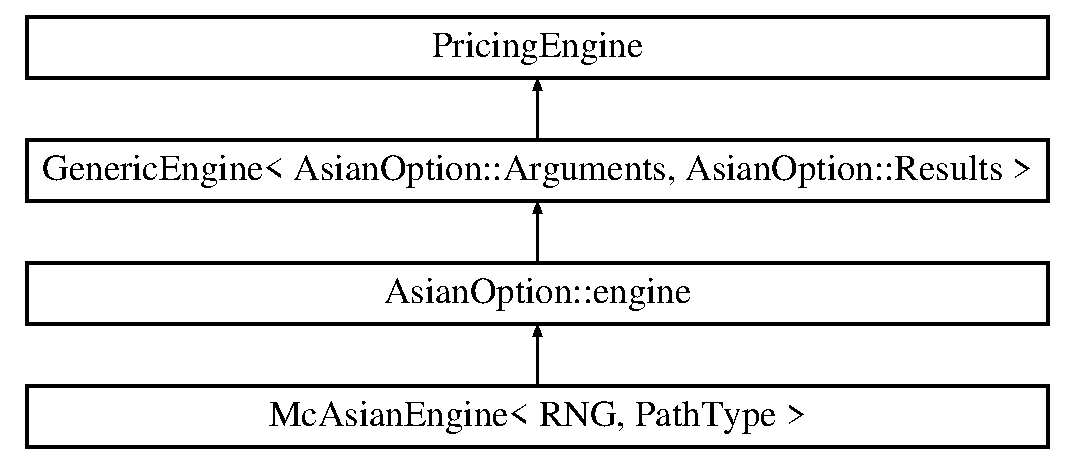
\includegraphics[height=4.000000cm]{class_asian_option_1_1engine}
\end{center}
\end{figure}
\subsection*{Additional Inherited Members}


The documentation for this class was generated from the following file\+:\begin{DoxyCompactItemize}
\item 
Instruments/\hyperlink{_asian_option_8h}{Asian\+Option.\+h}\end{DoxyCompactItemize}

\hypertarget{class_forward_1_1engine}{}\section{Forward\+:\+:engine Class Reference}
\label{class_forward_1_1engine}\index{Forward\+::engine@{Forward\+::engine}}
Inheritance diagram for Forward\+:\+:engine\+:\begin{figure}[H]
\begin{center}
\leavevmode
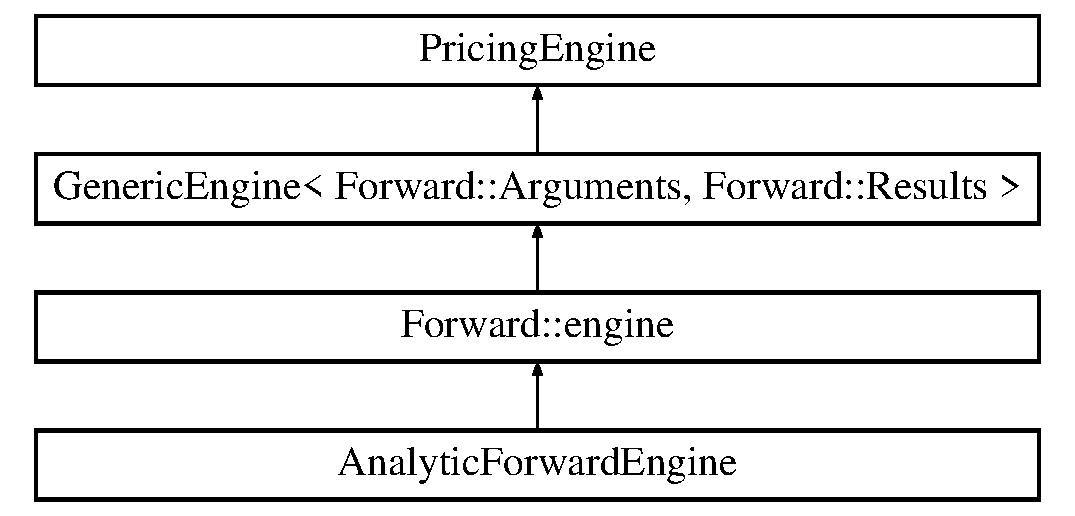
\includegraphics[height=4.000000cm]{class_forward_1_1engine}
\end{center}
\end{figure}
\subsection*{Additional Inherited Members}


The documentation for this class was generated from the following file\+:\begin{DoxyCompactItemize}
\item 
Users/\+C\+U\+I/\+Dropbox/\+C++/\+Finance/\+Instruments/Forward.\+h\end{DoxyCompactItemize}

\hypertarget{class_european_option}{}\section{European\+Option Class Reference}
\label{class_european_option}\index{European\+Option@{European\+Option}}


{\ttfamily \#include $<$European\+Option.\+h$>$}

Inheritance diagram for European\+Option\+:\begin{figure}[H]
\begin{center}
\leavevmode
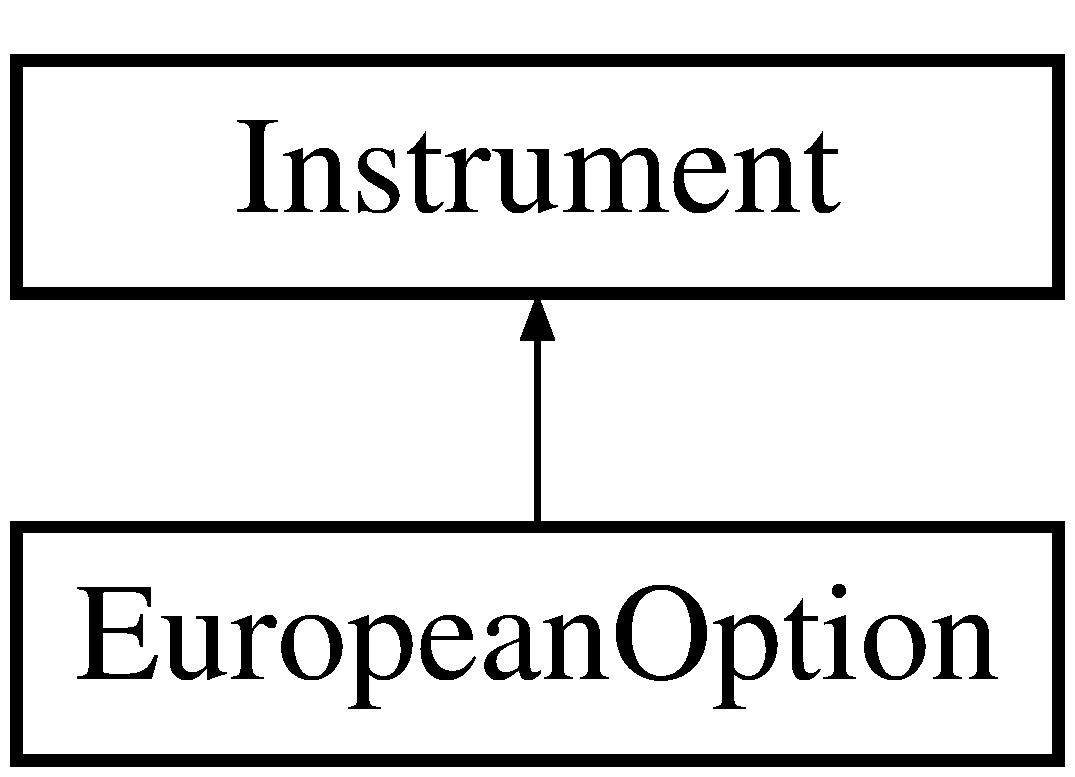
\includegraphics[height=2.000000cm]{class_european_option}
\end{center}
\end{figure}
\subsection*{Classes}
\begin{DoxyCompactItemize}
\item 
class \hyperlink{class_european_option_1_1_arguments}{Arguments}
\item 
class \hyperlink{class_european_option_1_1engine}{engine}
\item 
class \hyperlink{class_european_option_1_1_results}{Results}
\end{DoxyCompactItemize}
\subsection*{Public Member Functions}
\begin{DoxyCompactItemize}
\item 
\hyperlink{class_european_option_a92132b61922cb628bc355d4d9f302513}{European\+Option} (\hyperlink{_name_def_8h_ac2d3e0ba793497bcca555c7c2cf64ff3}{Time} maturity, std\+::shared\+\_\+ptr$<$ \hyperlink{class_payoff}{Payoff} $>$ payoff)
\item 
void \hyperlink{class_european_option_a94c1826feba0099400bce8dd6fc01cb9}{setup\+Arguments} (\hyperlink{class_pricing_engine_1_1_arguments}{Pricing\+Engine\+::\+Arguments} $\ast$arg) const override
\item 
\hyperlink{_name_def_8h_a5a9d48c16a694e9a2d9f1eca730dc8c5}{Money} \hyperlink{class_european_option_ae234d562ef21dc24c25f1538860da1cf}{fetch\+Results} (\hyperlink{class_pricing_engine_1_1_results}{Pricing\+Engine\+::\+Results} $\ast$const res) override
\end{DoxyCompactItemize}
\subsection*{Private Attributes}
\begin{DoxyCompactItemize}
\item 
std\+::shared\+\_\+ptr$<$ \hyperlink{class_payoff}{Payoff} $>$ \hyperlink{class_european_option_a3d597cb0b811f69a08e49b1af13b5a04}{payoff\+\_\+}
\item 
\hyperlink{_name_def_8h_ac2d3e0ba793497bcca555c7c2cf64ff3}{Time} \hyperlink{class_european_option_a8853b9bd1af9abc371630ae1c68f304c}{maturity\+\_\+}
\item 
std\+::shared\+\_\+ptr$<$ \hyperlink{class_european_option_1_1_results}{Results} $>$ \hyperlink{class_european_option_a228f13a5ce4c46caef1e3052b4a27610}{results\+\_\+}
\end{DoxyCompactItemize}
\subsection*{Additional Inherited Members}


\subsection{Constructor \& Destructor Documentation}
\hypertarget{class_european_option_a92132b61922cb628bc355d4d9f302513}{}\label{class_european_option_a92132b61922cb628bc355d4d9f302513} 
\index{European\+Option@{European\+Option}!European\+Option@{European\+Option}}
\index{European\+Option@{European\+Option}!European\+Option@{European\+Option}}
\subsubsection{\texorpdfstring{European\+Option()}{EuropeanOption()}}
{\footnotesize\ttfamily European\+Option\+::\+European\+Option (\begin{DoxyParamCaption}\item[{\hyperlink{_name_def_8h_ac2d3e0ba793497bcca555c7c2cf64ff3}{Time}}]{maturity,  }\item[{std\+::shared\+\_\+ptr$<$ \hyperlink{class_payoff}{Payoff} $>$}]{payoff }\end{DoxyParamCaption})}



\subsection{Member Function Documentation}
\hypertarget{class_european_option_ae234d562ef21dc24c25f1538860da1cf}{}\label{class_european_option_ae234d562ef21dc24c25f1538860da1cf} 
\index{European\+Option@{European\+Option}!fetch\+Results@{fetch\+Results}}
\index{fetch\+Results@{fetch\+Results}!European\+Option@{European\+Option}}
\subsubsection{\texorpdfstring{fetch\+Results()}{fetchResults()}}
{\footnotesize\ttfamily \hyperlink{_name_def_8h_a5a9d48c16a694e9a2d9f1eca730dc8c5}{Money} European\+Option\+::fetch\+Results (\begin{DoxyParamCaption}\item[{\hyperlink{class_pricing_engine_1_1_results}{Pricing\+Engine\+::\+Results} $\ast$const}]{res }\end{DoxyParamCaption})\hspace{0.3cm}{\ttfamily [override]}, {\ttfamily [virtual]}}



Implements \hyperlink{class_instrument_a381f093402f789ad7c0ffecd233167dc}{Instrument}.

\hypertarget{class_european_option_a94c1826feba0099400bce8dd6fc01cb9}{}\label{class_european_option_a94c1826feba0099400bce8dd6fc01cb9} 
\index{European\+Option@{European\+Option}!setup\+Arguments@{setup\+Arguments}}
\index{setup\+Arguments@{setup\+Arguments}!European\+Option@{European\+Option}}
\subsubsection{\texorpdfstring{setup\+Arguments()}{setupArguments()}}
{\footnotesize\ttfamily void European\+Option\+::setup\+Arguments (\begin{DoxyParamCaption}\item[{\hyperlink{class_pricing_engine_1_1_arguments}{Pricing\+Engine\+::\+Arguments} $\ast$}]{arg }\end{DoxyParamCaption}) const\hspace{0.3cm}{\ttfamily [override]}, {\ttfamily [virtual]}}



Implements \hyperlink{class_instrument_ac0f78fd32a360abde0c31b5bc01c7e67}{Instrument}.



\subsection{Member Data Documentation}
\hypertarget{class_european_option_a8853b9bd1af9abc371630ae1c68f304c}{}\label{class_european_option_a8853b9bd1af9abc371630ae1c68f304c} 
\index{European\+Option@{European\+Option}!maturity\+\_\+@{maturity\+\_\+}}
\index{maturity\+\_\+@{maturity\+\_\+}!European\+Option@{European\+Option}}
\subsubsection{\texorpdfstring{maturity\+\_\+}{maturity\_}}
{\footnotesize\ttfamily \hyperlink{_name_def_8h_ac2d3e0ba793497bcca555c7c2cf64ff3}{Time} European\+Option\+::maturity\+\_\+\hspace{0.3cm}{\ttfamily [private]}}

\hypertarget{class_european_option_a3d597cb0b811f69a08e49b1af13b5a04}{}\label{class_european_option_a3d597cb0b811f69a08e49b1af13b5a04} 
\index{European\+Option@{European\+Option}!payoff\+\_\+@{payoff\+\_\+}}
\index{payoff\+\_\+@{payoff\+\_\+}!European\+Option@{European\+Option}}
\subsubsection{\texorpdfstring{payoff\+\_\+}{payoff\_}}
{\footnotesize\ttfamily std\+::shared\+\_\+ptr$<$\hyperlink{class_payoff}{Payoff}$>$ European\+Option\+::payoff\+\_\+\hspace{0.3cm}{\ttfamily [private]}}

\hypertarget{class_european_option_a228f13a5ce4c46caef1e3052b4a27610}{}\label{class_european_option_a228f13a5ce4c46caef1e3052b4a27610} 
\index{European\+Option@{European\+Option}!results\+\_\+@{results\+\_\+}}
\index{results\+\_\+@{results\+\_\+}!European\+Option@{European\+Option}}
\subsubsection{\texorpdfstring{results\+\_\+}{results\_}}
{\footnotesize\ttfamily std\+::shared\+\_\+ptr$<$\hyperlink{class_european_option_1_1_results}{Results}$>$ European\+Option\+::results\+\_\+\hspace{0.3cm}{\ttfamily [private]}}



The documentation for this class was generated from the following files\+:\begin{DoxyCompactItemize}
\item 
Instruments/\hyperlink{_european_option_8h}{European\+Option.\+h}\item 
Instruments/\hyperlink{_european_option_8cpp}{European\+Option.\+cpp}\end{DoxyCompactItemize}

\hypertarget{class_european_path_pricer}{}\section{European\+Path\+Pricer Class Reference}
\label{class_european_path_pricer}\index{European\+Path\+Pricer@{European\+Path\+Pricer}}
Inheritance diagram for European\+Path\+Pricer\+:\begin{figure}[H]
\begin{center}
\leavevmode
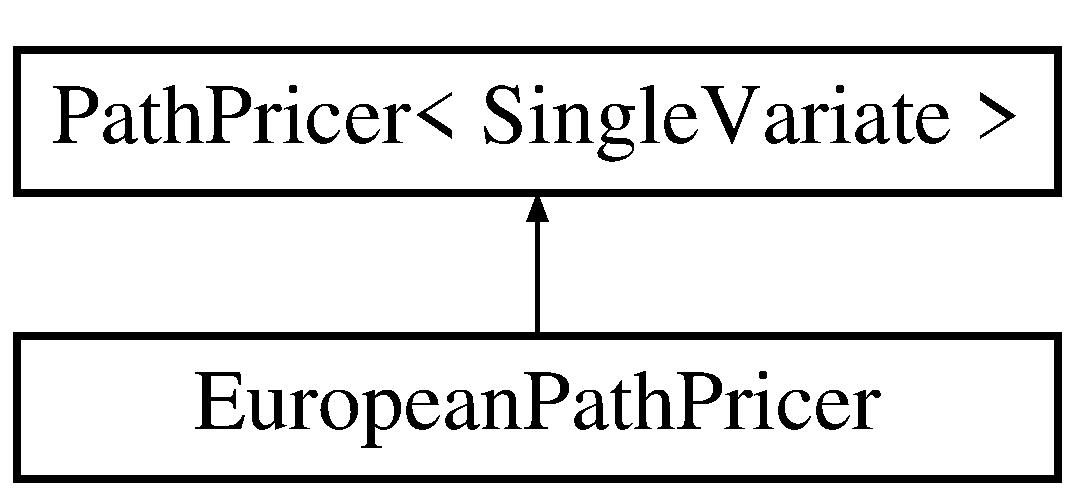
\includegraphics[height=2.000000cm]{class_european_path_pricer}
\end{center}
\end{figure}
\subsection*{Public Member Functions}
\begin{DoxyCompactItemize}
\item 
\hypertarget{class_european_path_pricer_aa571bb1652a0d7e4f97d3d58e7c8b295}{}\label{class_european_path_pricer_aa571bb1652a0d7e4f97d3d58e7c8b295} 
{\bfseries European\+Path\+Pricer} (const std\+::shared\+\_\+ptr$<$ \hyperlink{class_payoff}{Payoff} $>$ \&payoff, Rate discount)
\item 
\hypertarget{class_european_path_pricer_ac12142089ccdc7fe73ba93d66a7964e6}{}\label{class_european_path_pricer_ac12142089ccdc7fe73ba93d66a7964e6} 
Money {\bfseries operator()} (const \hyperlink{class_path}{Path} \&path) const override
\end{DoxyCompactItemize}


The documentation for this class was generated from the following files\+:\begin{DoxyCompactItemize}
\item 
Users/\+C\+U\+I/\+Dropbox/\+C++/\+Finance/\+Pricing\+Engines/European\+Path\+Pricer.\+h\item 
Users/\+C\+U\+I/\+Dropbox/\+C++/\+Finance/\+Pricing\+Engines/European\+Path\+Pricer.\+cpp\end{DoxyCompactItemize}

\hypertarget{class_forward}{}\section{Forward Class Reference}
\label{class_forward}\index{Forward@{Forward}}


{\ttfamily \#include $<$Forward.\+h$>$}

Inheritance diagram for Forward\+:\begin{figure}[H]
\begin{center}
\leavevmode
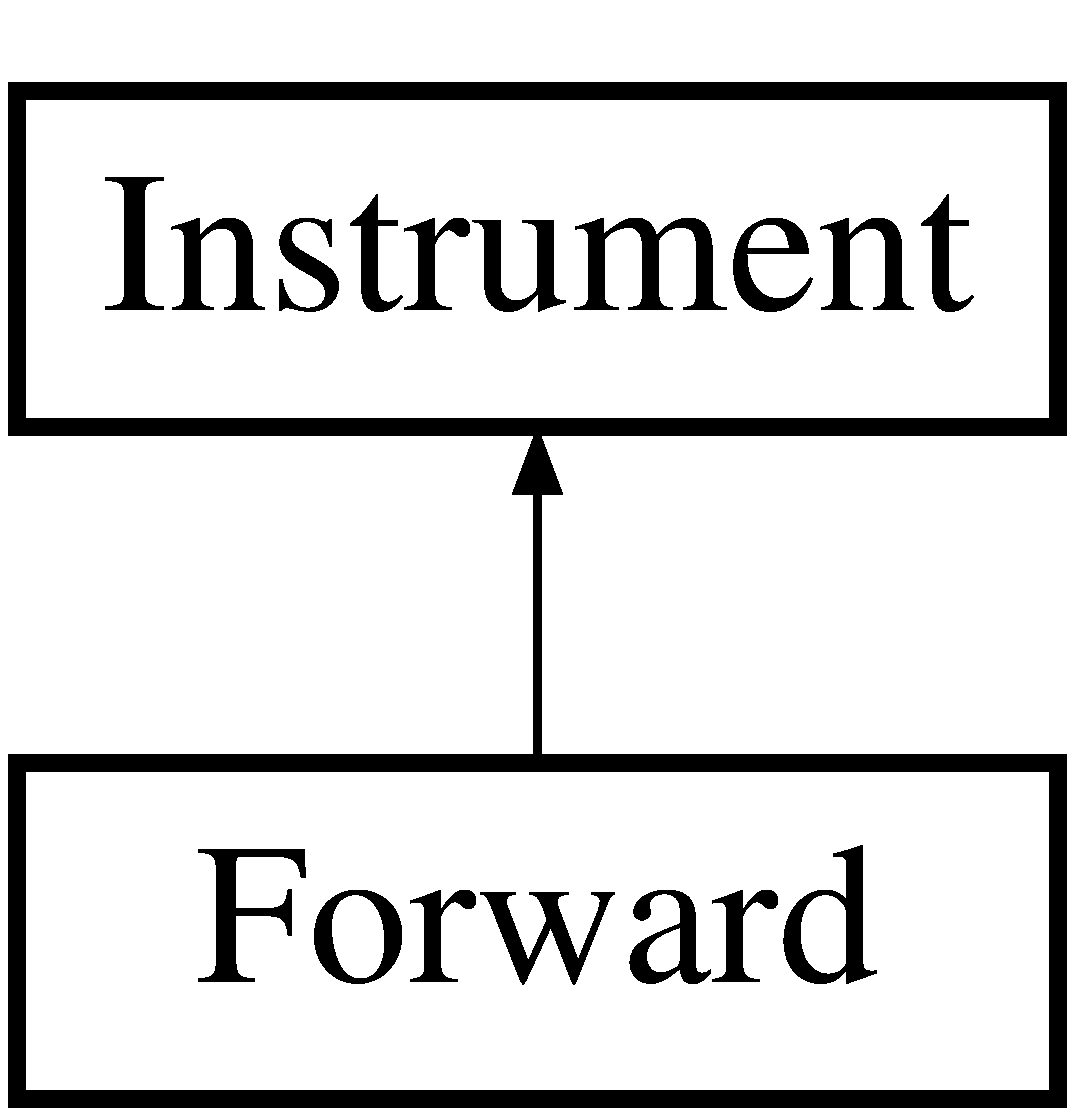
\includegraphics[height=2.000000cm]{class_forward}
\end{center}
\end{figure}
\subsection*{Classes}
\begin{DoxyCompactItemize}
\item 
class \hyperlink{class_forward_1_1_arguments}{Arguments}
\item 
class \hyperlink{class_forward_1_1engine}{engine}
\item 
class \hyperlink{class_forward_1_1_results}{Results}
\end{DoxyCompactItemize}
\subsection*{Public Member Functions}
\begin{DoxyCompactItemize}
\item 
\hyperlink{class_forward_a7ec14e1a089290cae0e70c4cddd353b5}{Forward} (\hyperlink{_name_def_8h_ac2d3e0ba793497bcca555c7c2cf64ff3}{Time} maturity, \hyperlink{_name_def_8h_a642a6c5fd87319d922637de0e0bb0305}{Quote} strike, \hyperlink{_name_def_8h_a642a6c5fd87319d922637de0e0bb0305}{Quote} spot)
\item 
void \hyperlink{class_forward_a909ab0cefa0ab42bdaf3bf6e84ac0096}{setup\+Arguments} (\hyperlink{class_pricing_engine_1_1_arguments}{Pricing\+Engine\+::\+Arguments} $\ast$const arg) const override
\begin{DoxyCompactList}\small\item\em To be called in method \hyperlink{class_instrument_aa750f2ae95a21d65a073da3171e8d084}{npv()} which is to setup all the arguments that are needed for pricing engine. \end{DoxyCompactList}\item 
\hyperlink{_name_def_8h_a5a9d48c16a694e9a2d9f1eca730dc8c5}{Money} \hyperlink{class_forward_ab1e2edeb8345c8605013634a598d1ae5}{fetch\+Results} (\hyperlink{class_pricing_engine_1_1_results}{Pricing\+Engine\+::\+Results} $\ast$const res) override
\begin{DoxyCompactList}\small\item\em To be called in method \hyperlink{class_instrument_aa750f2ae95a21d65a073da3171e8d084}{npv()} which is to get back the net present value after calculation. \end{DoxyCompactList}\end{DoxyCompactItemize}
\subsection*{Public Attributes}
\begin{DoxyCompactItemize}
\item 
std\+::shared\+\_\+ptr$<$ \hyperlink{class_forward_1_1_results}{Results} $>$ \hyperlink{class_forward_abead12e748980177fb67f98bcffbf817}{results\+\_\+}
\end{DoxyCompactItemize}
\subsection*{Private Attributes}
\begin{DoxyCompactItemize}
\item 
\hyperlink{_name_def_8h_a642a6c5fd87319d922637de0e0bb0305}{Quote} \hyperlink{class_forward_a17c32d0a673c13fd92288b1720a43b76}{strike\+\_\+}
\item 
\hyperlink{_name_def_8h_a642a6c5fd87319d922637de0e0bb0305}{Quote} \hyperlink{class_forward_a362d0396ceda462e504f77120339f8b0}{spot\+\_\+}
\item 
\hyperlink{_name_def_8h_ac2d3e0ba793497bcca555c7c2cf64ff3}{Time} \hyperlink{class_forward_ad599104a13c33fbf31e9214af904e9aa}{maturity\+\_\+}
\end{DoxyCompactItemize}
\subsection*{Additional Inherited Members}


\subsection{Constructor \& Destructor Documentation}
\hypertarget{class_forward_a7ec14e1a089290cae0e70c4cddd353b5}{}\label{class_forward_a7ec14e1a089290cae0e70c4cddd353b5} 
\index{Forward@{Forward}!Forward@{Forward}}
\index{Forward@{Forward}!Forward@{Forward}}
\subsubsection{\texorpdfstring{Forward()}{Forward()}}
{\footnotesize\ttfamily Forward\+::\+Forward (\begin{DoxyParamCaption}\item[{\hyperlink{_name_def_8h_ac2d3e0ba793497bcca555c7c2cf64ff3}{Time}}]{maturity,  }\item[{\hyperlink{_name_def_8h_a642a6c5fd87319d922637de0e0bb0305}{Quote}}]{strike,  }\item[{\hyperlink{_name_def_8h_a642a6c5fd87319d922637de0e0bb0305}{Quote}}]{spot }\end{DoxyParamCaption})}



\subsection{Member Function Documentation}
\hypertarget{class_forward_ab1e2edeb8345c8605013634a598d1ae5}{}\label{class_forward_ab1e2edeb8345c8605013634a598d1ae5} 
\index{Forward@{Forward}!fetch\+Results@{fetch\+Results}}
\index{fetch\+Results@{fetch\+Results}!Forward@{Forward}}
\subsubsection{\texorpdfstring{fetch\+Results()}{fetchResults()}}
{\footnotesize\ttfamily \hyperlink{_name_def_8h_a5a9d48c16a694e9a2d9f1eca730dc8c5}{Money} Forward\+::fetch\+Results (\begin{DoxyParamCaption}\item[{\hyperlink{class_pricing_engine_1_1_results}{Pricing\+Engine\+::\+Results} $\ast$const}]{res }\end{DoxyParamCaption})\hspace{0.3cm}{\ttfamily [override]}, {\ttfamily [virtual]}}



To be called in method \hyperlink{class_instrument_aa750f2ae95a21d65a073da3171e8d084}{npv()} which is to get back the net present value after calculation. 

{\itshape Constness\+:} Unlike setup\+Arguments, it is not a const member function. Result pointer res itself is const, but it does not point to const object. 
\begin{DoxyParams}{Parameters}
{\em res} & \hyperlink{class_forward_1_1_results}{Results} that are fetched back. \\
\hline
\end{DoxyParams}
\begin{DoxyReturn}{Returns}
Net present value after calculation. Other results are stored in the results class. 
\end{DoxyReturn}


Implements \hyperlink{class_instrument_a381f093402f789ad7c0ffecd233167dc}{Instrument}.

\hypertarget{class_forward_a909ab0cefa0ab42bdaf3bf6e84ac0096}{}\label{class_forward_a909ab0cefa0ab42bdaf3bf6e84ac0096} 
\index{Forward@{Forward}!setup\+Arguments@{setup\+Arguments}}
\index{setup\+Arguments@{setup\+Arguments}!Forward@{Forward}}
\subsubsection{\texorpdfstring{setup\+Arguments()}{setupArguments()}}
{\footnotesize\ttfamily void Forward\+::setup\+Arguments (\begin{DoxyParamCaption}\item[{\hyperlink{class_pricing_engine_1_1_arguments}{Pricing\+Engine\+::\+Arguments} $\ast$const}]{arg }\end{DoxyParamCaption}) const\hspace{0.3cm}{\ttfamily [override]}, {\ttfamily [virtual]}}



To be called in method \hyperlink{class_instrument_aa750f2ae95a21d65a073da3171e8d084}{npv()} which is to setup all the arguments that are needed for pricing engine. 

{\itshape Constness\+:} Const member function. Argument pointer arg itself is const, but it does not point to const object. 
\begin{DoxyParams}{Parameters}
{\em arg} & \hyperlink{class_forward_1_1_arguments}{Arguments} that are needed for pricing engine. \\
\hline
\end{DoxyParams}


Implements \hyperlink{class_instrument_a5cd384be384fe415f09ecc78e2a87539}{Instrument}.



\subsection{Member Data Documentation}
\hypertarget{class_forward_ad599104a13c33fbf31e9214af904e9aa}{}\label{class_forward_ad599104a13c33fbf31e9214af904e9aa} 
\index{Forward@{Forward}!maturity\+\_\+@{maturity\+\_\+}}
\index{maturity\+\_\+@{maturity\+\_\+}!Forward@{Forward}}
\subsubsection{\texorpdfstring{maturity\+\_\+}{maturity\_}}
{\footnotesize\ttfamily \hyperlink{_name_def_8h_ac2d3e0ba793497bcca555c7c2cf64ff3}{Time} Forward\+::maturity\+\_\+\hspace{0.3cm}{\ttfamily [private]}}

\hypertarget{class_forward_abead12e748980177fb67f98bcffbf817}{}\label{class_forward_abead12e748980177fb67f98bcffbf817} 
\index{Forward@{Forward}!results\+\_\+@{results\+\_\+}}
\index{results\+\_\+@{results\+\_\+}!Forward@{Forward}}
\subsubsection{\texorpdfstring{results\+\_\+}{results\_}}
{\footnotesize\ttfamily std\+::shared\+\_\+ptr$<$\hyperlink{class_forward_1_1_results}{Results}$>$ Forward\+::results\+\_\+}

\hypertarget{class_forward_a362d0396ceda462e504f77120339f8b0}{}\label{class_forward_a362d0396ceda462e504f77120339f8b0} 
\index{Forward@{Forward}!spot\+\_\+@{spot\+\_\+}}
\index{spot\+\_\+@{spot\+\_\+}!Forward@{Forward}}
\subsubsection{\texorpdfstring{spot\+\_\+}{spot\_}}
{\footnotesize\ttfamily \hyperlink{_name_def_8h_a642a6c5fd87319d922637de0e0bb0305}{Quote} Forward\+::spot\+\_\+\hspace{0.3cm}{\ttfamily [private]}}

\hypertarget{class_forward_a17c32d0a673c13fd92288b1720a43b76}{}\label{class_forward_a17c32d0a673c13fd92288b1720a43b76} 
\index{Forward@{Forward}!strike\+\_\+@{strike\+\_\+}}
\index{strike\+\_\+@{strike\+\_\+}!Forward@{Forward}}
\subsubsection{\texorpdfstring{strike\+\_\+}{strike\_}}
{\footnotesize\ttfamily \hyperlink{_name_def_8h_a642a6c5fd87319d922637de0e0bb0305}{Quote} Forward\+::strike\+\_\+\hspace{0.3cm}{\ttfamily [private]}}



The documentation for this class was generated from the following files\+:\begin{DoxyCompactItemize}
\item 
Instruments/\hyperlink{_forward_8h}{Forward.\+h}\item 
Instruments/\hyperlink{_forward_8cpp}{Forward.\+cpp}\end{DoxyCompactItemize}

\hypertarget{class_generic_engine}{}\section{Generic\+Engine$<$ Arguments\+Type, Results\+Type $>$ Class Template Reference}
\label{class_generic_engine}\index{Generic\+Engine$<$ Arguments\+Type, Results\+Type $>$@{Generic\+Engine$<$ Arguments\+Type, Results\+Type $>$}}


{\ttfamily \#include $<$Pricing\+Engine.\+h$>$}

Inheritance diagram for Generic\+Engine$<$ Arguments\+Type, Results\+Type $>$\+:\begin{figure}[H]
\begin{center}
\leavevmode
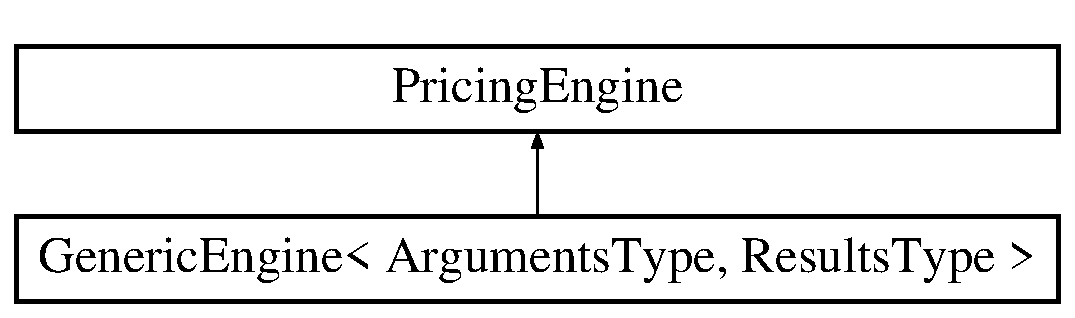
\includegraphics[height=2.000000cm]{class_generic_engine}
\end{center}
\end{figure}
\subsection*{Public Member Functions}
\begin{DoxyCompactItemize}
\item 
\hyperlink{class_generic_engine_a080b4df876712b5529b4a19ec3b0c48f}{Generic\+Engine} ()
\item 
\hyperlink{class_pricing_engine_1_1_arguments}{Pricing\+Engine\+::\+Arguments} $\ast$ \hyperlink{class_generic_engine_ac2adcbbc8d7b554e2cc1f90e4c4d055d}{get\+Arguments} () const override
\item 
\hyperlink{class_pricing_engine_1_1_results}{Pricing\+Engine\+::\+Results} $\ast$ \hyperlink{class_generic_engine_a2b8d7fba7e51c0795ea9f1e9c2f54afd}{get\+Results} () const override
\end{DoxyCompactItemize}
\subsection*{Public Attributes}
\begin{DoxyCompactItemize}
\item 
Arguments\+Type \hyperlink{class_generic_engine_a9ac595191e5d6976c65659d26063bfc8}{arguments\+\_\+}
\item 
Results\+Type \hyperlink{class_generic_engine_acd6af7c4b3fd0e43826755ba7d347dd5}{results\+\_\+}
\end{DoxyCompactItemize}


\subsection{Constructor \& Destructor Documentation}
\hypertarget{class_generic_engine_a080b4df876712b5529b4a19ec3b0c48f}{}\label{class_generic_engine_a080b4df876712b5529b4a19ec3b0c48f} 
\index{Generic\+Engine@{Generic\+Engine}!Generic\+Engine@{Generic\+Engine}}
\index{Generic\+Engine@{Generic\+Engine}!Generic\+Engine@{Generic\+Engine}}
\subsubsection{\texorpdfstring{Generic\+Engine()}{GenericEngine()}}
{\footnotesize\ttfamily template$<$typename Arguments\+Type, typename Results\+Type$>$ \\
\hyperlink{class_generic_engine}{Generic\+Engine}$<$ Arguments\+Type, Results\+Type $>$\+::\hyperlink{class_generic_engine}{Generic\+Engine} (\begin{DoxyParamCaption}{ }\end{DoxyParamCaption})\hspace{0.3cm}{\ttfamily [inline]}}



\subsection{Member Function Documentation}
\hypertarget{class_generic_engine_ac2adcbbc8d7b554e2cc1f90e4c4d055d}{}\label{class_generic_engine_ac2adcbbc8d7b554e2cc1f90e4c4d055d} 
\index{Generic\+Engine@{Generic\+Engine}!get\+Arguments@{get\+Arguments}}
\index{get\+Arguments@{get\+Arguments}!Generic\+Engine@{Generic\+Engine}}
\subsubsection{\texorpdfstring{get\+Arguments()}{getArguments()}}
{\footnotesize\ttfamily template$<$typename Arguments\+Type, typename Results\+Type$>$ \\
\hyperlink{class_pricing_engine_1_1_arguments}{Pricing\+Engine\+::\+Arguments}$\ast$ \hyperlink{class_generic_engine}{Generic\+Engine}$<$ Arguments\+Type, Results\+Type $>$\+::get\+Arguments (\begin{DoxyParamCaption}{ }\end{DoxyParamCaption}) const\hspace{0.3cm}{\ttfamily [inline]}, {\ttfamily [override]}, {\ttfamily [virtual]}}



Implements \hyperlink{class_pricing_engine_a399f4519f58b2ac1d108ce14d0058c97}{Pricing\+Engine}.

\hypertarget{class_generic_engine_a2b8d7fba7e51c0795ea9f1e9c2f54afd}{}\label{class_generic_engine_a2b8d7fba7e51c0795ea9f1e9c2f54afd} 
\index{Generic\+Engine@{Generic\+Engine}!get\+Results@{get\+Results}}
\index{get\+Results@{get\+Results}!Generic\+Engine@{Generic\+Engine}}
\subsubsection{\texorpdfstring{get\+Results()}{getResults()}}
{\footnotesize\ttfamily template$<$typename Arguments\+Type, typename Results\+Type$>$ \\
\hyperlink{class_pricing_engine_1_1_results}{Pricing\+Engine\+::\+Results}$\ast$ \hyperlink{class_generic_engine}{Generic\+Engine}$<$ Arguments\+Type, Results\+Type $>$\+::get\+Results (\begin{DoxyParamCaption}{ }\end{DoxyParamCaption}) const\hspace{0.3cm}{\ttfamily [inline]}, {\ttfamily [override]}, {\ttfamily [virtual]}}



Implements \hyperlink{class_pricing_engine_a73e2852ef4c28e92a402492e86717d0b}{Pricing\+Engine}.



\subsection{Member Data Documentation}
\hypertarget{class_generic_engine_a9ac595191e5d6976c65659d26063bfc8}{}\label{class_generic_engine_a9ac595191e5d6976c65659d26063bfc8} 
\index{Generic\+Engine@{Generic\+Engine}!arguments\+\_\+@{arguments\+\_\+}}
\index{arguments\+\_\+@{arguments\+\_\+}!Generic\+Engine@{Generic\+Engine}}
\subsubsection{\texorpdfstring{arguments\+\_\+}{arguments\_}}
{\footnotesize\ttfamily template$<$typename Arguments\+Type, typename Results\+Type$>$ \\
Arguments\+Type \hyperlink{class_generic_engine}{Generic\+Engine}$<$ Arguments\+Type, Results\+Type $>$\+::arguments\+\_\+\hspace{0.3cm}{\ttfamily [mutable]}}

\hypertarget{class_generic_engine_acd6af7c4b3fd0e43826755ba7d347dd5}{}\label{class_generic_engine_acd6af7c4b3fd0e43826755ba7d347dd5} 
\index{Generic\+Engine@{Generic\+Engine}!results\+\_\+@{results\+\_\+}}
\index{results\+\_\+@{results\+\_\+}!Generic\+Engine@{Generic\+Engine}}
\subsubsection{\texorpdfstring{results\+\_\+}{results\_}}
{\footnotesize\ttfamily template$<$typename Arguments\+Type, typename Results\+Type$>$ \\
Results\+Type \hyperlink{class_generic_engine}{Generic\+Engine}$<$ Arguments\+Type, Results\+Type $>$\+::results\+\_\+\hspace{0.3cm}{\ttfamily [mutable]}}



The documentation for this class was generated from the following file\+:\begin{DoxyCompactItemize}
\item 
Users/\+C\+U\+I/\+Dropbox/\+C++/\+Finance/\hyperlink{_pricing_engine_8h}{Pricing\+Engine.\+h}\end{DoxyCompactItemize}

\hypertarget{class_instrument}{}\section{Instrument Class Reference}
\label{class_instrument}\index{Instrument@{Instrument}}


Base \hyperlink{class_instrument}{Instrument} class.  




{\ttfamily \#include $<$Instrument.\+h$>$}

Inheritance diagram for Instrument\+:\begin{figure}[H]
\begin{center}
\leavevmode
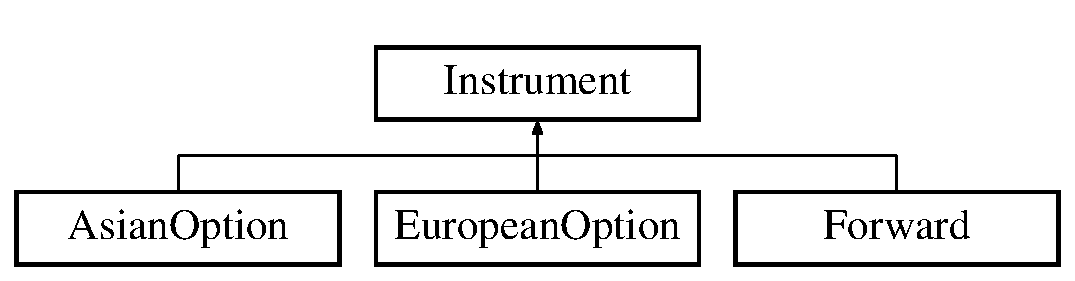
\includegraphics[height=2.000000cm]{class_instrument}
\end{center}
\end{figure}
\subsection*{Public Member Functions}
\begin{DoxyCompactItemize}
\item 
\hyperlink{_name_def_8h_a5a9d48c16a694e9a2d9f1eca730dc8c5}{Money} \hyperlink{class_instrument_aa750f2ae95a21d65a073da3171e8d084}{npv} ()
\begin{DoxyCompactList}\small\item\em Calculate the net present value by using the attached pricing engine. \end{DoxyCompactList}\item 
void \hyperlink{class_instrument_a47bdaa9390ab5e0616e8499a507c50cd}{set\+Pricing\+Engine} (const std\+::shared\+\_\+ptr$<$ \hyperlink{class_pricing_engine}{Pricing\+Engine} $>$ pricing\+Engine)
\begin{DoxyCompactList}\small\item\em Set the corresponding pricing engine. \end{DoxyCompactList}\end{DoxyCompactItemize}
\subsection*{Protected Member Functions}
\begin{DoxyCompactItemize}
\item 
virtual void \hyperlink{class_instrument_a5cd384be384fe415f09ecc78e2a87539}{setup\+Arguments} (\hyperlink{class_pricing_engine_1_1_arguments}{Pricing\+Engine\+::\+Arguments} $\ast$const arg) const =0
\begin{DoxyCompactList}\small\item\em To be called in method \hyperlink{class_instrument_aa750f2ae95a21d65a073da3171e8d084}{npv()} which is to setup all the arguments that are needed for pricing engine. \end{DoxyCompactList}\item 
virtual \hyperlink{_name_def_8h_a5a9d48c16a694e9a2d9f1eca730dc8c5}{Money} \hyperlink{class_instrument_a381f093402f789ad7c0ffecd233167dc}{fetch\+Results} (\hyperlink{class_pricing_engine_1_1_results}{Pricing\+Engine\+::\+Results} $\ast$const res)=0
\begin{DoxyCompactList}\small\item\em To be called in method \hyperlink{class_instrument_aa750f2ae95a21d65a073da3171e8d084}{npv()} which is to get back the net present value after calculation. \end{DoxyCompactList}\end{DoxyCompactItemize}
\subsection*{Protected Attributes}
\begin{DoxyCompactItemize}
\item 
std\+::shared\+\_\+ptr$<$ \hyperlink{class_pricing_engine}{Pricing\+Engine} $>$ \hyperlink{class_instrument_a6fdd5548ccc944536ff73913d98bf598}{pricing\+Engine\+\_\+}
\begin{DoxyCompactList}\small\item\em One pricing engine also can be used for other instrument, so shared\+\_\+ptr is used here. \end{DoxyCompactList}\end{DoxyCompactItemize}


\subsection{Detailed Description}
Base \hyperlink{class_instrument}{Instrument} class. 

This \hyperlink{class_instrument}{Instrument} class is an abstract base class for any financial instruments, like options, forward, swap, swaption, etc. There is always a set of \hyperlink{class_pricing_engine}{Pricing\+Engine} associated to each kind of instrument that can be used to price. Any inherited financial instrument classes should override the methods that are used to communicate the pricing\+Engines. 

\subsection{Member Function Documentation}
\hypertarget{class_instrument_a381f093402f789ad7c0ffecd233167dc}{}\label{class_instrument_a381f093402f789ad7c0ffecd233167dc} 
\index{Instrument@{Instrument}!fetch\+Results@{fetch\+Results}}
\index{fetch\+Results@{fetch\+Results}!Instrument@{Instrument}}
\subsubsection{\texorpdfstring{fetch\+Results()}{fetchResults()}}
{\footnotesize\ttfamily virtual \hyperlink{_name_def_8h_a5a9d48c16a694e9a2d9f1eca730dc8c5}{Money} Instrument\+::fetch\+Results (\begin{DoxyParamCaption}\item[{\hyperlink{class_pricing_engine_1_1_results}{Pricing\+Engine\+::\+Results} $\ast$const}]{res }\end{DoxyParamCaption})\hspace{0.3cm}{\ttfamily [protected]}, {\ttfamily [pure virtual]}}



To be called in method \hyperlink{class_instrument_aa750f2ae95a21d65a073da3171e8d084}{npv()} which is to get back the net present value after calculation. 

{\itshape Constness\+:} Unlike setup\+Arguments, it is not a const member function. Result pointer res itself is const, but it does not point to const object. 
\begin{DoxyParams}{Parameters}
{\em res} & Results that are fetched back. \\
\hline
\end{DoxyParams}
\begin{DoxyReturn}{Returns}
Net present value after calculation. Other results are stored in the results class. 
\end{DoxyReturn}


Implemented in \hyperlink{class_asian_option_a99cd9956b73d99a64748c913dcccd6ea}{Asian\+Option}, \hyperlink{class_forward_ab1e2edeb8345c8605013634a598d1ae5}{Forward}, and \hyperlink{class_european_option_ae234d562ef21dc24c25f1538860da1cf}{European\+Option}.

\hypertarget{class_instrument_aa750f2ae95a21d65a073da3171e8d084}{}\label{class_instrument_aa750f2ae95a21d65a073da3171e8d084} 
\index{Instrument@{Instrument}!npv@{npv}}
\index{npv@{npv}!Instrument@{Instrument}}
\subsubsection{\texorpdfstring{npv()}{npv()}}
{\footnotesize\ttfamily \hyperlink{_name_def_8h_a5a9d48c16a694e9a2d9f1eca730dc8c5}{Money} Instrument\+::npv (\begin{DoxyParamCaption}{ }\end{DoxyParamCaption})}



Calculate the net present value by using the attached pricing engine. 

Implemented by template pattern. ~\newline
Set the argument of \hyperlink{class_pricing_engine}{Pricing\+Engine} first and then calculate the npv by calling the method of \hyperlink{class_pricing_engine}{Pricing\+Engine} and finally fetch the results back from the \hyperlink{class_pricing_engine}{Pricing\+Engine} class. \hypertarget{class_instrument_a47bdaa9390ab5e0616e8499a507c50cd}{}\label{class_instrument_a47bdaa9390ab5e0616e8499a507c50cd} 
\index{Instrument@{Instrument}!set\+Pricing\+Engine@{set\+Pricing\+Engine}}
\index{set\+Pricing\+Engine@{set\+Pricing\+Engine}!Instrument@{Instrument}}
\subsubsection{\texorpdfstring{set\+Pricing\+Engine()}{setPricingEngine()}}
{\footnotesize\ttfamily void Instrument\+::set\+Pricing\+Engine (\begin{DoxyParamCaption}\item[{const std\+::shared\+\_\+ptr$<$ \hyperlink{class_pricing_engine}{Pricing\+Engine} $>$}]{pricing\+Engine }\end{DoxyParamCaption})}



Set the corresponding pricing engine. 

{\itshape Constness\+:} Pricing engine will not change. 
\begin{DoxyParams}{Parameters}
{\em pricing\+Engine} & The pricing engine to be used for pricing. ~\newline
\\
\hline
\end{DoxyParams}
\hypertarget{class_instrument_a5cd384be384fe415f09ecc78e2a87539}{}\label{class_instrument_a5cd384be384fe415f09ecc78e2a87539} 
\index{Instrument@{Instrument}!setup\+Arguments@{setup\+Arguments}}
\index{setup\+Arguments@{setup\+Arguments}!Instrument@{Instrument}}
\subsubsection{\texorpdfstring{setup\+Arguments()}{setupArguments()}}
{\footnotesize\ttfamily virtual void Instrument\+::setup\+Arguments (\begin{DoxyParamCaption}\item[{\hyperlink{class_pricing_engine_1_1_arguments}{Pricing\+Engine\+::\+Arguments} $\ast$const}]{arg }\end{DoxyParamCaption}) const\hspace{0.3cm}{\ttfamily [protected]}, {\ttfamily [pure virtual]}}



To be called in method \hyperlink{class_instrument_aa750f2ae95a21d65a073da3171e8d084}{npv()} which is to setup all the arguments that are needed for pricing engine. 

{\itshape Constness\+:} Const member function. Argument pointer arg itself is const, but it does not point to const object. 
\begin{DoxyParams}{Parameters}
{\em arg} & Arguments that are needed for pricing engine. \\
\hline
\end{DoxyParams}


Implemented in \hyperlink{class_asian_option_a82c9b5fb3bea69f476a65e9675e1cc28}{Asian\+Option}, \hyperlink{class_forward_a909ab0cefa0ab42bdaf3bf6e84ac0096}{Forward}, and \hyperlink{class_european_option_a77e3bc17dbcf317561c4920f6bfa84de}{European\+Option}.



\subsection{Member Data Documentation}
\hypertarget{class_instrument_a6fdd5548ccc944536ff73913d98bf598}{}\label{class_instrument_a6fdd5548ccc944536ff73913d98bf598} 
\index{Instrument@{Instrument}!pricing\+Engine\+\_\+@{pricing\+Engine\+\_\+}}
\index{pricing\+Engine\+\_\+@{pricing\+Engine\+\_\+}!Instrument@{Instrument}}
\subsubsection{\texorpdfstring{pricing\+Engine\+\_\+}{pricingEngine\_}}
{\footnotesize\ttfamily std\+::shared\+\_\+ptr$<$\hyperlink{class_pricing_engine}{Pricing\+Engine}$>$ Instrument\+::pricing\+Engine\+\_\+\hspace{0.3cm}{\ttfamily [protected]}}



One pricing engine also can be used for other instrument, so shared\+\_\+ptr is used here. 



The documentation for this class was generated from the following files\+:\begin{DoxyCompactItemize}
\item 
\hyperlink{_instrument_8h}{Instrument.\+h}\item 
\hyperlink{_instrument_8cpp}{Instrument.\+cpp}\end{DoxyCompactItemize}

\hypertarget{class_l_m_m}{}\section{L\+MM Class Reference}
\label{class_l_m_m}\index{L\+MM@{L\+MM}}


Standard \hyperlink{class_l_m_m}{L\+MM} model.  




{\ttfamily \#include $<$L\+M\+M.\+h$>$}

Inheritance diagram for L\+MM\+:\begin{figure}[H]
\begin{center}
\leavevmode
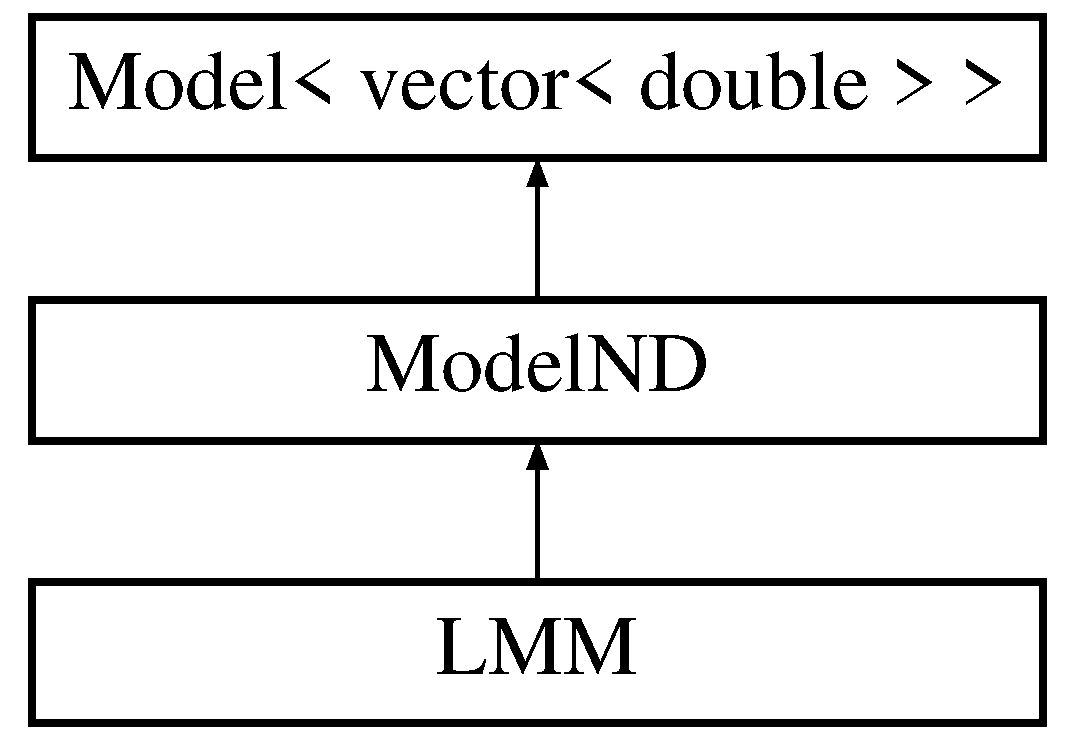
\includegraphics[height=3.000000cm]{class_l_m_m}
\end{center}
\end{figure}
\subsection*{Public Member Functions}
\begin{DoxyCompactItemize}
\item 
\hyperlink{class_l_m_m_a4de26d3647b221d5d16667a402edfef2}{L\+MM} ()=default
\item 
\hyperlink{class_l_m_m_aa6d3ff98a4153869dd59c17135181a4c}{L\+MM} (unsigned long dimension, const std\+::vector$<$ \hyperlink{_name_def_8h_a642a6c5fd87319d922637de0e0bb0305}{Quote} $>$ \&initial, unsigned long dim\+Vol, const std\+::vector$<$ std\+::shared\+\_\+ptr$<$ \hyperlink{class_parameter}{Parameter} $>$ $>$ \&params, \hyperlink{_name_def_8h_ac2d3e0ba793497bcca555c7c2cf64ff3}{Time} tenor)
\item 
std\+::vector$<$ \hyperlink{_name_def_8h_a642a6c5fd87319d922637de0e0bb0305}{Quote} $>$ \hyperlink{class_l_m_m_a8dfdd340048e482a8059f473b5aacfd1}{evolve} (\hyperlink{_name_def_8h_ac2d3e0ba793497bcca555c7c2cf64ff3}{Time} t0, std\+::vector$<$ \hyperlink{_name_def_8h_a642a6c5fd87319d922637de0e0bb0305}{Quote} $>$ \&x0, \hyperlink{_name_def_8h_ac2d3e0ba793497bcca555c7c2cf64ff3}{Time} dt, double dw) const override
\end{DoxyCompactItemize}
\subsection*{Private Attributes}
\begin{DoxyCompactItemize}
\item 
\hyperlink{_name_def_8h_ac2d3e0ba793497bcca555c7c2cf64ff3}{Time} \hyperlink{class_l_m_m_a92e55b5b940238e97a668c039cc593fa}{tenor\+\_\+}
\end{DoxyCompactItemize}
\subsection*{Additional Inherited Members}


\subsection{Detailed Description}
Standard \hyperlink{class_l_m_m}{L\+MM} model. 

This is the most standard Libor market model before financial crisis. The log-\/normal processes without stochastic multipliers are imposed in the dynamics of the \hyperlink{class_l_m_m}{L\+MM} model. 

\subsection{Constructor \& Destructor Documentation}
\hypertarget{class_l_m_m_a4de26d3647b221d5d16667a402edfef2}{}\label{class_l_m_m_a4de26d3647b221d5d16667a402edfef2} 
\index{L\+MM@{L\+MM}!L\+MM@{L\+MM}}
\index{L\+MM@{L\+MM}!L\+MM@{L\+MM}}
\subsubsection{\texorpdfstring{L\+M\+M()}{LMM()}\hspace{0.1cm}{\footnotesize\ttfamily [1/2]}}
{\footnotesize\ttfamily L\+M\+M\+::\+L\+MM (\begin{DoxyParamCaption}{ }\end{DoxyParamCaption})\hspace{0.3cm}{\ttfamily [default]}}

\hypertarget{class_l_m_m_aa6d3ff98a4153869dd59c17135181a4c}{}\label{class_l_m_m_aa6d3ff98a4153869dd59c17135181a4c} 
\index{L\+MM@{L\+MM}!L\+MM@{L\+MM}}
\index{L\+MM@{L\+MM}!L\+MM@{L\+MM}}
\subsubsection{\texorpdfstring{L\+M\+M()}{LMM()}\hspace{0.1cm}{\footnotesize\ttfamily [2/2]}}
{\footnotesize\ttfamily L\+M\+M\+::\+L\+MM (\begin{DoxyParamCaption}\item[{unsigned long}]{dimension,  }\item[{const std\+::vector$<$ \hyperlink{_name_def_8h_a642a6c5fd87319d922637de0e0bb0305}{Quote} $>$ \&}]{initial,  }\item[{unsigned long}]{dim\+Vol,  }\item[{const std\+::vector$<$ std\+::shared\+\_\+ptr$<$ \hyperlink{class_parameter}{Parameter} $>$ $>$ \&}]{params,  }\item[{\hyperlink{_name_def_8h_ac2d3e0ba793497bcca555c7c2cf64ff3}{Time}}]{tenor }\end{DoxyParamCaption})}


\begin{DoxyParams}{Parameters}
{\em dimension} & number of (riskfree) forward rates \\
\hline
{\em initial} & initial value at time 0 \\
\hline
{\em dim\+Vol} & volatility dimension of each dynamic \\
\hline
{\em params} & vector of needed parameters structure \\
\hline
{\em tenor} & tenor of forward rates, e.\+g. 1M(1/12), 3M(1/4), 6M(1/2), 12M(1) \\
\hline
\end{DoxyParams}
no check for the input 

\subsection{Member Function Documentation}
\hypertarget{class_l_m_m_a8dfdd340048e482a8059f473b5aacfd1}{}\label{class_l_m_m_a8dfdd340048e482a8059f473b5aacfd1} 
\index{L\+MM@{L\+MM}!evolve@{evolve}}
\index{evolve@{evolve}!L\+MM@{L\+MM}}
\subsubsection{\texorpdfstring{evolve()}{evolve()}}
{\footnotesize\ttfamily std\+::vector$<$\hyperlink{_name_def_8h_a642a6c5fd87319d922637de0e0bb0305}{Quote}$>$ L\+M\+M\+::evolve (\begin{DoxyParamCaption}\item[{\hyperlink{_name_def_8h_ac2d3e0ba793497bcca555c7c2cf64ff3}{Time}}]{t0,  }\item[{std\+::vector$<$ \hyperlink{_name_def_8h_a642a6c5fd87319d922637de0e0bb0305}{Quote} $>$ \&}]{x0,  }\item[{\hyperlink{_name_def_8h_ac2d3e0ba793497bcca555c7c2cf64ff3}{Time}}]{dt,  }\item[{double}]{dw }\end{DoxyParamCaption}) const\hspace{0.3cm}{\ttfamily [inline]}, {\ttfamily [override]}}



\subsection{Member Data Documentation}
\hypertarget{class_l_m_m_a92e55b5b940238e97a668c039cc593fa}{}\label{class_l_m_m_a92e55b5b940238e97a668c039cc593fa} 
\index{L\+MM@{L\+MM}!tenor\+\_\+@{tenor\+\_\+}}
\index{tenor\+\_\+@{tenor\+\_\+}!L\+MM@{L\+MM}}
\subsubsection{\texorpdfstring{tenor\+\_\+}{tenor\_}}
{\footnotesize\ttfamily \hyperlink{_name_def_8h_ac2d3e0ba793497bcca555c7c2cf64ff3}{Time} L\+M\+M\+::tenor\+\_\+\hspace{0.3cm}{\ttfamily [private]}}



The documentation for this class was generated from the following files\+:\begin{DoxyCompactItemize}
\item 
Models/\hyperlink{_l_m_m_8h}{L\+M\+M.\+h}\item 
Models/\hyperlink{_l_m_m_8cpp}{L\+M\+M.\+cpp}\end{DoxyCompactItemize}

\hypertarget{class_log_normal_process}{}\section{Log\+Normal\+Process$<$ Vol\+Type $>$ Class Template Reference}
\label{class_log_normal_process}\index{Log\+Normal\+Process$<$ Vol\+Type $>$@{Log\+Normal\+Process$<$ Vol\+Type $>$}}


{\ttfamily \#include $<$Log\+Normal\+Process.\+h$>$}

Inheritance diagram for Log\+Normal\+Process$<$ Vol\+Type $>$\+:\begin{figure}[H]
\begin{center}
\leavevmode
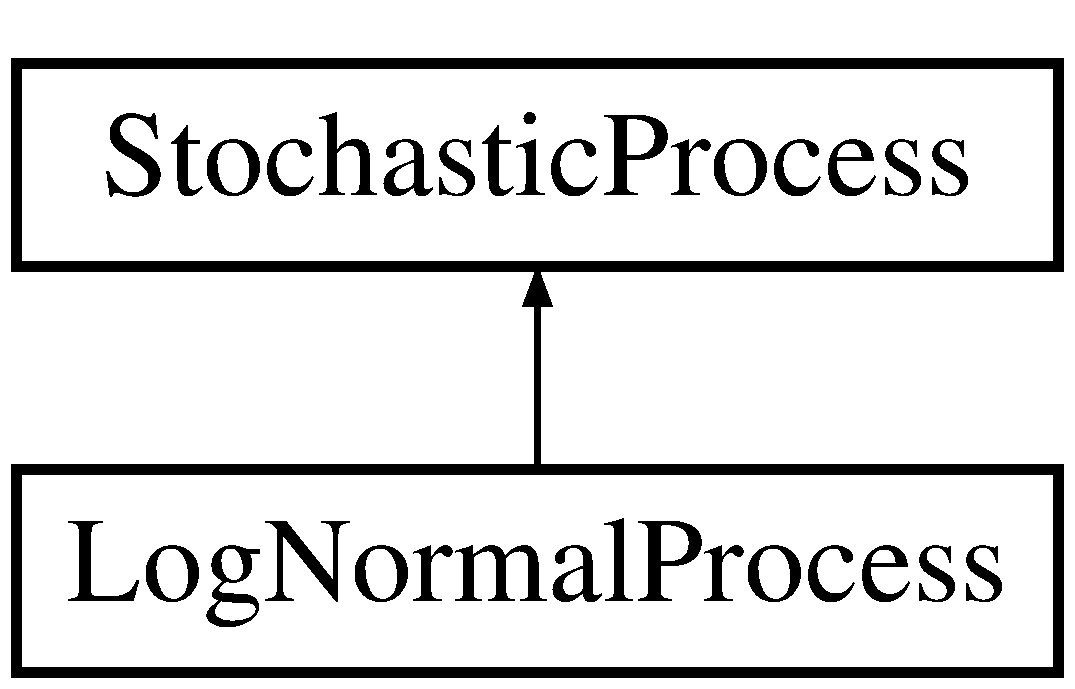
\includegraphics[height=3.000000cm]{class_log_normal_process}
\end{center}
\end{figure}
\subsection*{Public Types}
\begin{DoxyCompactItemize}
\item 
typedef Vol\+Type\+::vol\+\_\+return\+\_\+type \hyperlink{class_log_normal_process_a160d9cd152962a42ac9fc016d0948c1c}{vol\+\_\+return\+\_\+type}
\item 
typedef Vol\+Type\+::vol\+\_\+ptr\+\_\+type \hyperlink{class_log_normal_process_a904926553c5e4d60e52caf87e1745651}{vol\+\_\+ptr\+\_\+type}
\end{DoxyCompactItemize}
\subsection*{Public Member Functions}
\begin{DoxyCompactItemize}
\item 
\hyperlink{class_log_normal_process_acf4b8a29784c43d8c613d9707492179c}{Log\+Normal\+Process} ()=default
\item 
\hyperlink{class_log_normal_process_a1320686151d44d334be1289d21f1c711}{Log\+Normal\+Process} (\hyperlink{_name_def_8h_a642a6c5fd87319d922637de0e0bb0305}{Quote} x0, const shared\+\_\+ptr$<$ \hyperlink{class_parameter}{Parameter} $>$ \&drift, unsigned long dim\+Vol, const \hyperlink{class_log_normal_process_a904926553c5e4d60e52caf87e1745651}{vol\+\_\+ptr\+\_\+type} \&volatility)
\item 
virtual double \hyperlink{class_log_normal_process_a2c01b829c59e9b6156f0e34b3632c800}{get\+Spot} () const override
\item 
double \hyperlink{class_log_normal_process_a629e2612ff67a957accb04e5fe0ad2a9}{get\+Drift} (\hyperlink{_name_def_8h_ac2d3e0ba793497bcca555c7c2cf64ff3}{Time} t) const
\item 
shared\+\_\+ptr$<$ \hyperlink{class_parameter}{Parameter} $>$ \hyperlink{class_log_normal_process_a474db0a26169f742a61cb187347151ec}{get\+Drift} () const
\item 
virtual \hyperlink{class_log_normal_process_a160d9cd152962a42ac9fc016d0948c1c}{vol\+\_\+return\+\_\+type} \hyperlink{class_log_normal_process_af2d153f75cd5efbeaa3a9028585dd835}{get\+Volatility} (\hyperlink{_name_def_8h_ac2d3e0ba793497bcca555c7c2cf64ff3}{Time} t) const
\item 
shared\+\_\+ptr$<$ \hyperlink{class_parameter}{Parameter} $>$ \hyperlink{class_log_normal_process_a7860abf96c754c037531680cb0dde6ff}{get\+Volatility} () const
\item 
unsigned long \hyperlink{class_log_normal_process_a708854438eccd5ed5d1a996c5f0b6ff8}{get\+Vol\+Dimension} () const
\end{DoxyCompactItemize}
\subsection*{Protected Member Functions}
\begin{DoxyCompactItemize}
\item 
double \hyperlink{class_log_normal_process_a547e799140c1575cc979416f3cf7ab24}{get\+Vol\+Helper} (const shared\+\_\+ptr$<$ \hyperlink{class_parameter}{Parameter} $>$ vol, \hyperlink{_name_def_8h_ac2d3e0ba793497bcca555c7c2cf64ff3}{Time} t) const
\item 
vector$<$ double $>$ \hyperlink{class_log_normal_process_aa65ab0e1f6b6679f49e993dfd1d3e9a0}{get\+Vol\+Helper} (const vector$<$ shared\+\_\+ptr$<$ \hyperlink{class_parameter}{Parameter} $>$$>$ vols, \hyperlink{_name_def_8h_ac2d3e0ba793497bcca555c7c2cf64ff3}{Time} t) const
\end{DoxyCompactItemize}
\subsection*{Protected Attributes}
\begin{DoxyCompactItemize}
\item 
\hyperlink{_name_def_8h_a642a6c5fd87319d922637de0e0bb0305}{Quote} \hyperlink{class_log_normal_process_aaad6cd95af55b1d573fa384ddb0066ef}{x0\+\_\+}
\item 
shared\+\_\+ptr$<$ \hyperlink{class_parameter}{Parameter} $>$ \hyperlink{class_log_normal_process_ae59abec9b1917c092665a99464f4af85}{drift\+\_\+}
\item 
unsigned long \hyperlink{class_log_normal_process_ae126cc386f39576fa62debd75443fa08}{dim\+Vol\+\_\+}
\item 
\hyperlink{class_log_normal_process_a904926553c5e4d60e52caf87e1745651}{vol\+\_\+ptr\+\_\+type} \hyperlink{class_log_normal_process_a90615a4b65992ad6fb280b18a9a705b3}{volatility\+\_\+}
\end{DoxyCompactItemize}


\subsection{Member Typedef Documentation}
\hypertarget{class_log_normal_process_a904926553c5e4d60e52caf87e1745651}{}\label{class_log_normal_process_a904926553c5e4d60e52caf87e1745651} 
\index{Log\+Normal\+Process@{Log\+Normal\+Process}!vol\+\_\+ptr\+\_\+type@{vol\+\_\+ptr\+\_\+type}}
\index{vol\+\_\+ptr\+\_\+type@{vol\+\_\+ptr\+\_\+type}!Log\+Normal\+Process@{Log\+Normal\+Process}}
\subsubsection{\texorpdfstring{vol\+\_\+ptr\+\_\+type}{vol\_ptr\_type}}
{\footnotesize\ttfamily template$<$typename Vol\+Type$>$ \\
typedef Vol\+Type\+::vol\+\_\+ptr\+\_\+type \hyperlink{class_log_normal_process}{Log\+Normal\+Process}$<$ Vol\+Type $>$\+::\hyperlink{class_log_normal_process_a904926553c5e4d60e52caf87e1745651}{vol\+\_\+ptr\+\_\+type}}

\hypertarget{class_log_normal_process_a160d9cd152962a42ac9fc016d0948c1c}{}\label{class_log_normal_process_a160d9cd152962a42ac9fc016d0948c1c} 
\index{Log\+Normal\+Process@{Log\+Normal\+Process}!vol\+\_\+return\+\_\+type@{vol\+\_\+return\+\_\+type}}
\index{vol\+\_\+return\+\_\+type@{vol\+\_\+return\+\_\+type}!Log\+Normal\+Process@{Log\+Normal\+Process}}
\subsubsection{\texorpdfstring{vol\+\_\+return\+\_\+type}{vol\_return\_type}}
{\footnotesize\ttfamily template$<$typename Vol\+Type$>$ \\
typedef Vol\+Type\+::vol\+\_\+return\+\_\+type \hyperlink{class_log_normal_process}{Log\+Normal\+Process}$<$ Vol\+Type $>$\+::\hyperlink{class_log_normal_process_a160d9cd152962a42ac9fc016d0948c1c}{vol\+\_\+return\+\_\+type}}



\subsection{Constructor \& Destructor Documentation}
\hypertarget{class_log_normal_process_acf4b8a29784c43d8c613d9707492179c}{}\label{class_log_normal_process_acf4b8a29784c43d8c613d9707492179c} 
\index{Log\+Normal\+Process@{Log\+Normal\+Process}!Log\+Normal\+Process@{Log\+Normal\+Process}}
\index{Log\+Normal\+Process@{Log\+Normal\+Process}!Log\+Normal\+Process@{Log\+Normal\+Process}}
\subsubsection{\texorpdfstring{Log\+Normal\+Process()}{LogNormalProcess()}\hspace{0.1cm}{\footnotesize\ttfamily [1/2]}}
{\footnotesize\ttfamily template$<$typename Vol\+Type$>$ \\
\hyperlink{class_log_normal_process}{Log\+Normal\+Process}$<$ Vol\+Type $>$\+::\hyperlink{class_log_normal_process}{Log\+Normal\+Process} (\begin{DoxyParamCaption}{ }\end{DoxyParamCaption})\hspace{0.3cm}{\ttfamily [default]}}

\hypertarget{class_log_normal_process_a1320686151d44d334be1289d21f1c711}{}\label{class_log_normal_process_a1320686151d44d334be1289d21f1c711} 
\index{Log\+Normal\+Process@{Log\+Normal\+Process}!Log\+Normal\+Process@{Log\+Normal\+Process}}
\index{Log\+Normal\+Process@{Log\+Normal\+Process}!Log\+Normal\+Process@{Log\+Normal\+Process}}
\subsubsection{\texorpdfstring{Log\+Normal\+Process()}{LogNormalProcess()}\hspace{0.1cm}{\footnotesize\ttfamily [2/2]}}
{\footnotesize\ttfamily template$<$typename Vol\+Type$>$ \\
\hyperlink{class_log_normal_process}{Log\+Normal\+Process}$<$ Vol\+Type $>$\+::\hyperlink{class_log_normal_process}{Log\+Normal\+Process} (\begin{DoxyParamCaption}\item[{\hyperlink{_name_def_8h_a642a6c5fd87319d922637de0e0bb0305}{Quote}}]{x0,  }\item[{const shared\+\_\+ptr$<$ \hyperlink{class_parameter}{Parameter} $>$ \&}]{drift,  }\item[{unsigned long}]{dim\+Vol,  }\item[{const \hyperlink{class_log_normal_process_a904926553c5e4d60e52caf87e1745651}{vol\+\_\+ptr\+\_\+type} \&}]{volatility }\end{DoxyParamCaption})}



\subsection{Member Function Documentation}
\hypertarget{class_log_normal_process_a629e2612ff67a957accb04e5fe0ad2a9}{}\label{class_log_normal_process_a629e2612ff67a957accb04e5fe0ad2a9} 
\index{Log\+Normal\+Process@{Log\+Normal\+Process}!get\+Drift@{get\+Drift}}
\index{get\+Drift@{get\+Drift}!Log\+Normal\+Process@{Log\+Normal\+Process}}
\subsubsection{\texorpdfstring{get\+Drift()}{getDrift()}\hspace{0.1cm}{\footnotesize\ttfamily [1/2]}}
{\footnotesize\ttfamily template$<$typename Vol\+Type $>$ \\
double \hyperlink{class_log_normal_process}{Log\+Normal\+Process}$<$ Vol\+Type $>$\+::get\+Drift (\begin{DoxyParamCaption}\item[{\hyperlink{_name_def_8h_ac2d3e0ba793497bcca555c7c2cf64ff3}{Time}}]{t }\end{DoxyParamCaption}) const}

\hypertarget{class_log_normal_process_a474db0a26169f742a61cb187347151ec}{}\label{class_log_normal_process_a474db0a26169f742a61cb187347151ec} 
\index{Log\+Normal\+Process@{Log\+Normal\+Process}!get\+Drift@{get\+Drift}}
\index{get\+Drift@{get\+Drift}!Log\+Normal\+Process@{Log\+Normal\+Process}}
\subsubsection{\texorpdfstring{get\+Drift()}{getDrift()}\hspace{0.1cm}{\footnotesize\ttfamily [2/2]}}
{\footnotesize\ttfamily template$<$typename Vol\+Type$>$ \\
shared\+\_\+ptr$<$\hyperlink{class_parameter}{Parameter}$>$ \hyperlink{class_log_normal_process}{Log\+Normal\+Process}$<$ Vol\+Type $>$\+::get\+Drift (\begin{DoxyParamCaption}{ }\end{DoxyParamCaption}) const\hspace{0.3cm}{\ttfamily [inline]}}

\hypertarget{class_log_normal_process_a2c01b829c59e9b6156f0e34b3632c800}{}\label{class_log_normal_process_a2c01b829c59e9b6156f0e34b3632c800} 
\index{Log\+Normal\+Process@{Log\+Normal\+Process}!get\+Spot@{get\+Spot}}
\index{get\+Spot@{get\+Spot}!Log\+Normal\+Process@{Log\+Normal\+Process}}
\subsubsection{\texorpdfstring{get\+Spot()}{getSpot()}}
{\footnotesize\ttfamily template$<$typename Vol\+Type$>$ \\
virtual double \hyperlink{class_log_normal_process}{Log\+Normal\+Process}$<$ Vol\+Type $>$\+::get\+Spot (\begin{DoxyParamCaption}{ }\end{DoxyParamCaption}) const\hspace{0.3cm}{\ttfamily [inline]}, {\ttfamily [override]}, {\ttfamily [virtual]}}



Implements \hyperlink{class_stochastic_process_aad2ef51ca4bc2fe5f33a73e8f0ee361e}{Stochastic\+Process}.



Reimplemented in \hyperlink{class_log_normal_with_normal_jump_a7a6cd6409ac252d9c68ecbc36e135fb5}{Log\+Normal\+With\+Normal\+Jump$<$ Vol\+Type $>$}.

\hypertarget{class_log_normal_process_af2d153f75cd5efbeaa3a9028585dd835}{}\label{class_log_normal_process_af2d153f75cd5efbeaa3a9028585dd835} 
\index{Log\+Normal\+Process@{Log\+Normal\+Process}!get\+Volatility@{get\+Volatility}}
\index{get\+Volatility@{get\+Volatility}!Log\+Normal\+Process@{Log\+Normal\+Process}}
\subsubsection{\texorpdfstring{get\+Volatility()}{getVolatility()}\hspace{0.1cm}{\footnotesize\ttfamily [1/2]}}
{\footnotesize\ttfamily template$<$typename Vol\+Type $>$ \\
\hyperlink{class_log_normal_process}{Log\+Normal\+Process}$<$ Vol\+Type $>$\+::\hyperlink{class_log_normal_process_a160d9cd152962a42ac9fc016d0948c1c}{vol\+\_\+return\+\_\+type} \hyperlink{class_log_normal_process}{Log\+Normal\+Process}$<$ Vol\+Type $>$\+::get\+Volatility (\begin{DoxyParamCaption}\item[{\hyperlink{_name_def_8h_ac2d3e0ba793497bcca555c7c2cf64ff3}{Time}}]{t }\end{DoxyParamCaption}) const\hspace{0.3cm}{\ttfamily [virtual]}}



Reimplemented in \hyperlink{class_b_s_stochastic_process_ad20afb9e82ee123452a7d828837289f6}{B\+S\+Stochastic\+Process}.

\hypertarget{class_log_normal_process_a7860abf96c754c037531680cb0dde6ff}{}\label{class_log_normal_process_a7860abf96c754c037531680cb0dde6ff} 
\index{Log\+Normal\+Process@{Log\+Normal\+Process}!get\+Volatility@{get\+Volatility}}
\index{get\+Volatility@{get\+Volatility}!Log\+Normal\+Process@{Log\+Normal\+Process}}
\subsubsection{\texorpdfstring{get\+Volatility()}{getVolatility()}\hspace{0.1cm}{\footnotesize\ttfamily [2/2]}}
{\footnotesize\ttfamily template$<$typename Vol\+Type$>$ \\
shared\+\_\+ptr$<$\hyperlink{class_parameter}{Parameter}$>$ \hyperlink{class_log_normal_process}{Log\+Normal\+Process}$<$ Vol\+Type $>$\+::get\+Volatility (\begin{DoxyParamCaption}{ }\end{DoxyParamCaption}) const\hspace{0.3cm}{\ttfamily [inline]}}

\hypertarget{class_log_normal_process_a708854438eccd5ed5d1a996c5f0b6ff8}{}\label{class_log_normal_process_a708854438eccd5ed5d1a996c5f0b6ff8} 
\index{Log\+Normal\+Process@{Log\+Normal\+Process}!get\+Vol\+Dimension@{get\+Vol\+Dimension}}
\index{get\+Vol\+Dimension@{get\+Vol\+Dimension}!Log\+Normal\+Process@{Log\+Normal\+Process}}
\subsubsection{\texorpdfstring{get\+Vol\+Dimension()}{getVolDimension()}}
{\footnotesize\ttfamily template$<$typename Vol\+Type$>$ \\
unsigned long \hyperlink{class_log_normal_process}{Log\+Normal\+Process}$<$ Vol\+Type $>$\+::get\+Vol\+Dimension (\begin{DoxyParamCaption}{ }\end{DoxyParamCaption}) const\hspace{0.3cm}{\ttfamily [inline]}}

\hypertarget{class_log_normal_process_a547e799140c1575cc979416f3cf7ab24}{}\label{class_log_normal_process_a547e799140c1575cc979416f3cf7ab24} 
\index{Log\+Normal\+Process@{Log\+Normal\+Process}!get\+Vol\+Helper@{get\+Vol\+Helper}}
\index{get\+Vol\+Helper@{get\+Vol\+Helper}!Log\+Normal\+Process@{Log\+Normal\+Process}}
\subsubsection{\texorpdfstring{get\+Vol\+Helper()}{getVolHelper()}\hspace{0.1cm}{\footnotesize\ttfamily [1/2]}}
{\footnotesize\ttfamily template$<$typename Vol\+Type $>$ \\
double \hyperlink{class_log_normal_process}{Log\+Normal\+Process}$<$ Vol\+Type $>$\+::get\+Vol\+Helper (\begin{DoxyParamCaption}\item[{const shared\+\_\+ptr$<$ \hyperlink{class_parameter}{Parameter} $>$}]{vol,  }\item[{\hyperlink{_name_def_8h_ac2d3e0ba793497bcca555c7c2cf64ff3}{Time}}]{t }\end{DoxyParamCaption}) const\hspace{0.3cm}{\ttfamily [protected]}}

\hypertarget{class_log_normal_process_aa65ab0e1f6b6679f49e993dfd1d3e9a0}{}\label{class_log_normal_process_aa65ab0e1f6b6679f49e993dfd1d3e9a0} 
\index{Log\+Normal\+Process@{Log\+Normal\+Process}!get\+Vol\+Helper@{get\+Vol\+Helper}}
\index{get\+Vol\+Helper@{get\+Vol\+Helper}!Log\+Normal\+Process@{Log\+Normal\+Process}}
\subsubsection{\texorpdfstring{get\+Vol\+Helper()}{getVolHelper()}\hspace{0.1cm}{\footnotesize\ttfamily [2/2]}}
{\footnotesize\ttfamily template$<$typename Vol\+Type $>$ \\
vector$<$ double $>$ \hyperlink{class_log_normal_process}{Log\+Normal\+Process}$<$ Vol\+Type $>$\+::get\+Vol\+Helper (\begin{DoxyParamCaption}\item[{const vector$<$ shared\+\_\+ptr$<$ \hyperlink{class_parameter}{Parameter} $>$$>$}]{vols,  }\item[{\hyperlink{_name_def_8h_ac2d3e0ba793497bcca555c7c2cf64ff3}{Time}}]{t }\end{DoxyParamCaption}) const\hspace{0.3cm}{\ttfamily [protected]}}



\subsection{Member Data Documentation}
\hypertarget{class_log_normal_process_ae126cc386f39576fa62debd75443fa08}{}\label{class_log_normal_process_ae126cc386f39576fa62debd75443fa08} 
\index{Log\+Normal\+Process@{Log\+Normal\+Process}!dim\+Vol\+\_\+@{dim\+Vol\+\_\+}}
\index{dim\+Vol\+\_\+@{dim\+Vol\+\_\+}!Log\+Normal\+Process@{Log\+Normal\+Process}}
\subsubsection{\texorpdfstring{dim\+Vol\+\_\+}{dimVol\_}}
{\footnotesize\ttfamily template$<$typename Vol\+Type$>$ \\
unsigned long \hyperlink{class_log_normal_process}{Log\+Normal\+Process}$<$ Vol\+Type $>$\+::dim\+Vol\+\_\+\hspace{0.3cm}{\ttfamily [protected]}}

\hypertarget{class_log_normal_process_ae59abec9b1917c092665a99464f4af85}{}\label{class_log_normal_process_ae59abec9b1917c092665a99464f4af85} 
\index{Log\+Normal\+Process@{Log\+Normal\+Process}!drift\+\_\+@{drift\+\_\+}}
\index{drift\+\_\+@{drift\+\_\+}!Log\+Normal\+Process@{Log\+Normal\+Process}}
\subsubsection{\texorpdfstring{drift\+\_\+}{drift\_}}
{\footnotesize\ttfamily template$<$typename Vol\+Type$>$ \\
shared\+\_\+ptr$<$\hyperlink{class_parameter}{Parameter}$>$ \hyperlink{class_log_normal_process}{Log\+Normal\+Process}$<$ Vol\+Type $>$\+::drift\+\_\+\hspace{0.3cm}{\ttfamily [protected]}}

\hypertarget{class_log_normal_process_a90615a4b65992ad6fb280b18a9a705b3}{}\label{class_log_normal_process_a90615a4b65992ad6fb280b18a9a705b3} 
\index{Log\+Normal\+Process@{Log\+Normal\+Process}!volatility\+\_\+@{volatility\+\_\+}}
\index{volatility\+\_\+@{volatility\+\_\+}!Log\+Normal\+Process@{Log\+Normal\+Process}}
\subsubsection{\texorpdfstring{volatility\+\_\+}{volatility\_}}
{\footnotesize\ttfamily template$<$typename Vol\+Type$>$ \\
\hyperlink{class_log_normal_process_a904926553c5e4d60e52caf87e1745651}{vol\+\_\+ptr\+\_\+type} \hyperlink{class_log_normal_process}{Log\+Normal\+Process}$<$ Vol\+Type $>$\+::volatility\+\_\+\hspace{0.3cm}{\ttfamily [protected]}}

\hypertarget{class_log_normal_process_aaad6cd95af55b1d573fa384ddb0066ef}{}\label{class_log_normal_process_aaad6cd95af55b1d573fa384ddb0066ef} 
\index{Log\+Normal\+Process@{Log\+Normal\+Process}!x0\+\_\+@{x0\+\_\+}}
\index{x0\+\_\+@{x0\+\_\+}!Log\+Normal\+Process@{Log\+Normal\+Process}}
\subsubsection{\texorpdfstring{x0\+\_\+}{x0\_}}
{\footnotesize\ttfamily template$<$typename Vol\+Type$>$ \\
\hyperlink{_name_def_8h_a642a6c5fd87319d922637de0e0bb0305}{Quote} \hyperlink{class_log_normal_process}{Log\+Normal\+Process}$<$ Vol\+Type $>$\+::x0\+\_\+\hspace{0.3cm}{\ttfamily [protected]}}



The documentation for this class was generated from the following file\+:\begin{DoxyCompactItemize}
\item 
Stochastic\+Processes/\hyperlink{_log_normal_process_8h}{Log\+Normal\+Process.\+h}\end{DoxyCompactItemize}

\hypertarget{class_mc_asian_engine}{}\section{Mc\+Asian\+Engine$<$ Unif\+Rng $>$ Class Template Reference}
\label{class_mc_asian_engine}\index{Mc\+Asian\+Engine$<$ Unif\+Rng $>$@{Mc\+Asian\+Engine$<$ Unif\+Rng $>$}}


{\ttfamily \#include $<$Mc\+Asian\+Engine.\+h$>$}

Inheritance diagram for Mc\+Asian\+Engine$<$ Unif\+Rng $>$\+:\begin{figure}[H]
\begin{center}
\leavevmode
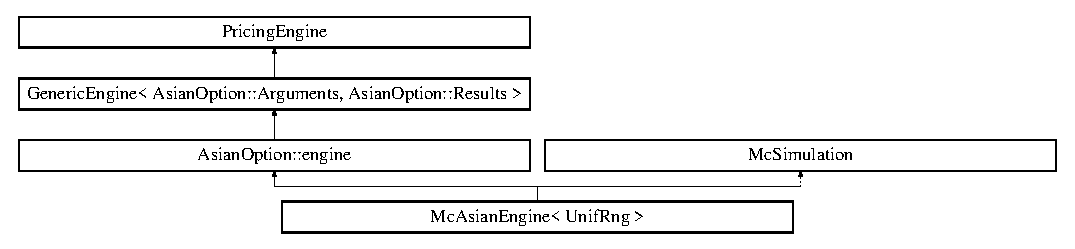
\includegraphics[height=2.894057cm]{class_mc_asian_engine}
\end{center}
\end{figure}
\subsection*{Public Member Functions}
\begin{DoxyCompactItemize}
\item 
\hyperlink{class_mc_asian_engine_a8688d15638d6176095dab92ef31ad3ad}{Mc\+Asian\+Engine} (const std\+::shared\+\_\+ptr$<$ \hyperlink{class_model}{Model} $>$ model, \hyperlink{_name_def_8h_ac2d3e0ba793497bcca555c7c2cf64ff3}{Time} time\+Step, unsigned long max\+Samples, unsigned long min\+Samples, bool is\+Antithetic=0)
\item 
std\+::shared\+\_\+ptr$<$ \hyperlink{class_path_generator}{Path\+Generator}$<$ \hyperlink{class_normal_marsaglia_bray_rng}{Normal\+Marsaglia\+Bray\+Rng}$<$ Unif\+Rng $>$ $>$ $>$ \hyperlink{class_mc_asian_engine_a93c9216b38bcbe0fe7e8131bf975dbc2}{path\+Generator} () override
\item 
std\+::shared\+\_\+ptr$<$ \hyperlink{class_path_pricer}{Path\+Pricer} $>$ \hyperlink{class_mc_asian_engine_afb903df1f8e0023a1f6bfae43ccbc8f7}{path\+Pricer} () override
\item 
vector$<$ \hyperlink{_name_def_8h_ac2d3e0ba793497bcca555c7c2cf64ff3}{Time} $>$ \hyperlink{class_mc_asian_engine_a4c16366e8dec7d689e934cbafe413332}{time\+Grid} () override
\item 
void \hyperlink{class_mc_asian_engine_a4e67149307de395f821c8aa07afad3b8}{calculate} () override
\end{DoxyCompactItemize}
\subsection*{Private Attributes}
\begin{DoxyCompactItemize}
\item 
std\+::shared\+\_\+ptr$<$ \hyperlink{class_model}{Model} $>$ \hyperlink{class_mc_asian_engine_a3b8579245987fd1a2f98561fee7e7011}{model\+\_\+}
\item 
unsigned long \hyperlink{class_mc_asian_engine_ad310118988d49cf73b5515ee6af85996}{min\+Samples\+\_\+}
\item 
unsigned long \hyperlink{class_mc_asian_engine_afef8e1a62d6d3e865a511f9b24bc16fe}{max\+Samples\+\_\+}
\item 
\hyperlink{_name_def_8h_ac2d3e0ba793497bcca555c7c2cf64ff3}{Time} \hyperlink{class_mc_asian_engine_a44bf438e294ec6b6475e85412422ec54}{time\+Step\+\_\+}
\item 
bool \hyperlink{class_mc_asian_engine_adbc09c299d05335c926179154fd52eca}{is\+Antithetic\+\_\+}
\end{DoxyCompactItemize}
\subsection*{Additional Inherited Members}


\subsection{Constructor \& Destructor Documentation}
\hypertarget{class_mc_asian_engine_a8688d15638d6176095dab92ef31ad3ad}{}\label{class_mc_asian_engine_a8688d15638d6176095dab92ef31ad3ad} 
\index{Mc\+Asian\+Engine@{Mc\+Asian\+Engine}!Mc\+Asian\+Engine@{Mc\+Asian\+Engine}}
\index{Mc\+Asian\+Engine@{Mc\+Asian\+Engine}!Mc\+Asian\+Engine@{Mc\+Asian\+Engine}}
\subsubsection{\texorpdfstring{Mc\+Asian\+Engine()}{McAsianEngine()}}
{\footnotesize\ttfamily template$<$typename Unif\+Rng $>$ \\
\hyperlink{class_mc_asian_engine}{Mc\+Asian\+Engine}$<$ Unif\+Rng $>$\+::\hyperlink{class_mc_asian_engine}{Mc\+Asian\+Engine} (\begin{DoxyParamCaption}\item[{const std\+::shared\+\_\+ptr$<$ \hyperlink{class_model}{Model} $>$}]{model,  }\item[{\hyperlink{_name_def_8h_ac2d3e0ba793497bcca555c7c2cf64ff3}{Time}}]{time\+Step,  }\item[{unsigned long}]{max\+Samples,  }\item[{unsigned long}]{min\+Samples,  }\item[{bool}]{is\+Antithetic = {\ttfamily 0} }\end{DoxyParamCaption})}



\subsection{Member Function Documentation}
\hypertarget{class_mc_asian_engine_a4e67149307de395f821c8aa07afad3b8}{}\label{class_mc_asian_engine_a4e67149307de395f821c8aa07afad3b8} 
\index{Mc\+Asian\+Engine@{Mc\+Asian\+Engine}!calculate@{calculate}}
\index{calculate@{calculate}!Mc\+Asian\+Engine@{Mc\+Asian\+Engine}}
\subsubsection{\texorpdfstring{calculate()}{calculate()}}
{\footnotesize\ttfamily template$<$typename Unif\+Rng $>$ \\
void \hyperlink{class_mc_asian_engine}{Mc\+Asian\+Engine}$<$ Unif\+Rng $>$\+::calculate (\begin{DoxyParamCaption}{ }\end{DoxyParamCaption})\hspace{0.3cm}{\ttfamily [override]}, {\ttfamily [virtual]}}



Implements \hyperlink{class_pricing_engine_a733511ffc3cf5e4dc1fbc2a39208d8bd}{Pricing\+Engine}.

\hypertarget{class_mc_asian_engine_a93c9216b38bcbe0fe7e8131bf975dbc2}{}\label{class_mc_asian_engine_a93c9216b38bcbe0fe7e8131bf975dbc2} 
\index{Mc\+Asian\+Engine@{Mc\+Asian\+Engine}!path\+Generator@{path\+Generator}}
\index{path\+Generator@{path\+Generator}!Mc\+Asian\+Engine@{Mc\+Asian\+Engine}}
\subsubsection{\texorpdfstring{path\+Generator()}{pathGenerator()}}
{\footnotesize\ttfamily template$<$typename Unif\+Rng $>$ \\
std\+::shared\+\_\+ptr$<$ \hyperlink{class_path_generator}{Path\+Generator}$<$ \hyperlink{class_normal_marsaglia_bray_rng}{Normal\+Marsaglia\+Bray\+Rng}$<$ Unif\+Rng $>$ $>$ $>$ \hyperlink{class_mc_asian_engine}{Mc\+Asian\+Engine}$<$ Unif\+Rng $>$\+::path\+Generator (\begin{DoxyParamCaption}{ }\end{DoxyParamCaption})\hspace{0.3cm}{\ttfamily [override]}, {\ttfamily [virtual]}}



Implements \hyperlink{class_mc_simulation_ada27dc346c81cf3d7aff84188dd12381}{Mc\+Simulation}.

\hypertarget{class_mc_asian_engine_afb903df1f8e0023a1f6bfae43ccbc8f7}{}\label{class_mc_asian_engine_afb903df1f8e0023a1f6bfae43ccbc8f7} 
\index{Mc\+Asian\+Engine@{Mc\+Asian\+Engine}!path\+Pricer@{path\+Pricer}}
\index{path\+Pricer@{path\+Pricer}!Mc\+Asian\+Engine@{Mc\+Asian\+Engine}}
\subsubsection{\texorpdfstring{path\+Pricer()}{pathPricer()}}
{\footnotesize\ttfamily template$<$typename Unif\+Rng $>$ \\
std\+::shared\+\_\+ptr$<$ \hyperlink{class_path_pricer}{Path\+Pricer} $>$ \hyperlink{class_mc_asian_engine}{Mc\+Asian\+Engine}$<$ Unif\+Rng $>$\+::path\+Pricer (\begin{DoxyParamCaption}{ }\end{DoxyParamCaption})\hspace{0.3cm}{\ttfamily [override]}, {\ttfamily [virtual]}}



Implements \hyperlink{class_mc_simulation_a3182a27c79d31cfb65e9a1a6b60f5391}{Mc\+Simulation}.

\hypertarget{class_mc_asian_engine_a4c16366e8dec7d689e934cbafe413332}{}\label{class_mc_asian_engine_a4c16366e8dec7d689e934cbafe413332} 
\index{Mc\+Asian\+Engine@{Mc\+Asian\+Engine}!time\+Grid@{time\+Grid}}
\index{time\+Grid@{time\+Grid}!Mc\+Asian\+Engine@{Mc\+Asian\+Engine}}
\subsubsection{\texorpdfstring{time\+Grid()}{timeGrid()}}
{\footnotesize\ttfamily template$<$typename Unif\+Rng $>$ \\
vector$<$ \hyperlink{_name_def_8h_ac2d3e0ba793497bcca555c7c2cf64ff3}{Time} $>$ \hyperlink{class_mc_asian_engine}{Mc\+Asian\+Engine}$<$ Unif\+Rng $>$\+::time\+Grid (\begin{DoxyParamCaption}{ }\end{DoxyParamCaption})\hspace{0.3cm}{\ttfamily [override]}, {\ttfamily [virtual]}}



Implements \hyperlink{class_mc_simulation_a71f4b6eedd90f057203a94467a691387}{Mc\+Simulation}.



\subsection{Member Data Documentation}
\hypertarget{class_mc_asian_engine_adbc09c299d05335c926179154fd52eca}{}\label{class_mc_asian_engine_adbc09c299d05335c926179154fd52eca} 
\index{Mc\+Asian\+Engine@{Mc\+Asian\+Engine}!is\+Antithetic\+\_\+@{is\+Antithetic\+\_\+}}
\index{is\+Antithetic\+\_\+@{is\+Antithetic\+\_\+}!Mc\+Asian\+Engine@{Mc\+Asian\+Engine}}
\subsubsection{\texorpdfstring{is\+Antithetic\+\_\+}{isAntithetic\_}}
{\footnotesize\ttfamily template$<$typename Unif\+Rng  = Uniform\+L\+Ecuyer\+R\+N\+G1$>$ \\
bool \hyperlink{class_mc_asian_engine}{Mc\+Asian\+Engine}$<$ Unif\+Rng $>$\+::is\+Antithetic\+\_\+\hspace{0.3cm}{\ttfamily [private]}}

\hypertarget{class_mc_asian_engine_afef8e1a62d6d3e865a511f9b24bc16fe}{}\label{class_mc_asian_engine_afef8e1a62d6d3e865a511f9b24bc16fe} 
\index{Mc\+Asian\+Engine@{Mc\+Asian\+Engine}!max\+Samples\+\_\+@{max\+Samples\+\_\+}}
\index{max\+Samples\+\_\+@{max\+Samples\+\_\+}!Mc\+Asian\+Engine@{Mc\+Asian\+Engine}}
\subsubsection{\texorpdfstring{max\+Samples\+\_\+}{maxSamples\_}}
{\footnotesize\ttfamily template$<$typename Unif\+Rng  = Uniform\+L\+Ecuyer\+R\+N\+G1$>$ \\
unsigned long \hyperlink{class_mc_asian_engine}{Mc\+Asian\+Engine}$<$ Unif\+Rng $>$\+::max\+Samples\+\_\+\hspace{0.3cm}{\ttfamily [private]}}

\hypertarget{class_mc_asian_engine_ad310118988d49cf73b5515ee6af85996}{}\label{class_mc_asian_engine_ad310118988d49cf73b5515ee6af85996} 
\index{Mc\+Asian\+Engine@{Mc\+Asian\+Engine}!min\+Samples\+\_\+@{min\+Samples\+\_\+}}
\index{min\+Samples\+\_\+@{min\+Samples\+\_\+}!Mc\+Asian\+Engine@{Mc\+Asian\+Engine}}
\subsubsection{\texorpdfstring{min\+Samples\+\_\+}{minSamples\_}}
{\footnotesize\ttfamily template$<$typename Unif\+Rng  = Uniform\+L\+Ecuyer\+R\+N\+G1$>$ \\
unsigned long \hyperlink{class_mc_asian_engine}{Mc\+Asian\+Engine}$<$ Unif\+Rng $>$\+::min\+Samples\+\_\+\hspace{0.3cm}{\ttfamily [private]}}

\hypertarget{class_mc_asian_engine_a3b8579245987fd1a2f98561fee7e7011}{}\label{class_mc_asian_engine_a3b8579245987fd1a2f98561fee7e7011} 
\index{Mc\+Asian\+Engine@{Mc\+Asian\+Engine}!model\+\_\+@{model\+\_\+}}
\index{model\+\_\+@{model\+\_\+}!Mc\+Asian\+Engine@{Mc\+Asian\+Engine}}
\subsubsection{\texorpdfstring{model\+\_\+}{model\_}}
{\footnotesize\ttfamily template$<$typename Unif\+Rng  = Uniform\+L\+Ecuyer\+R\+N\+G1$>$ \\
std\+::shared\+\_\+ptr$<$\hyperlink{class_model}{Model}$>$ \hyperlink{class_mc_asian_engine}{Mc\+Asian\+Engine}$<$ Unif\+Rng $>$\+::model\+\_\+\hspace{0.3cm}{\ttfamily [private]}}

\hypertarget{class_mc_asian_engine_a44bf438e294ec6b6475e85412422ec54}{}\label{class_mc_asian_engine_a44bf438e294ec6b6475e85412422ec54} 
\index{Mc\+Asian\+Engine@{Mc\+Asian\+Engine}!time\+Step\+\_\+@{time\+Step\+\_\+}}
\index{time\+Step\+\_\+@{time\+Step\+\_\+}!Mc\+Asian\+Engine@{Mc\+Asian\+Engine}}
\subsubsection{\texorpdfstring{time\+Step\+\_\+}{timeStep\_}}
{\footnotesize\ttfamily template$<$typename Unif\+Rng  = Uniform\+L\+Ecuyer\+R\+N\+G1$>$ \\
\hyperlink{_name_def_8h_ac2d3e0ba793497bcca555c7c2cf64ff3}{Time} \hyperlink{class_mc_asian_engine}{Mc\+Asian\+Engine}$<$ Unif\+Rng $>$\+::time\+Step\+\_\+\hspace{0.3cm}{\ttfamily [private]}}



The documentation for this class was generated from the following file\+:\begin{DoxyCompactItemize}
\item 
Pricing\+Engines/\hyperlink{_mc_asian_engine_8h}{Mc\+Asian\+Engine.\+h}\end{DoxyCompactItemize}

\hypertarget{class_mc_european_engine}{}\section{Mc\+European\+Engine$<$ R\+NG $>$ Class Template Reference}
\label{class_mc_european_engine}\index{Mc\+European\+Engine$<$ R\+N\+G $>$@{Mc\+European\+Engine$<$ R\+N\+G $>$}}


{\ttfamily \#include $<$M\+C\+European\+Engine.\+h$>$}

Inheritance diagram for Mc\+European\+Engine$<$ R\+NG $>$\+:\begin{figure}[H]
\begin{center}
\leavevmode
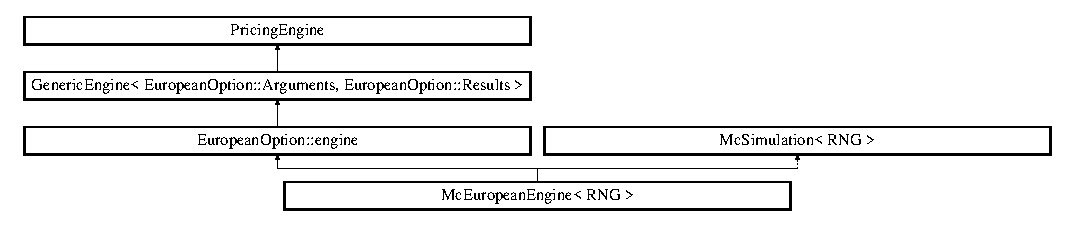
\includegraphics[height=2.586605cm]{class_mc_european_engine}
\end{center}
\end{figure}
\subsection*{Public Member Functions}
\begin{DoxyCompactItemize}
\item 
\hyperlink{class_mc_european_engine_a22424812ecaf6e04134eeaa45b9d1e1f}{Mc\+European\+Engine} (const std\+::shared\+\_\+ptr$<$ \hyperlink{class_model}{Model} $>$ model, \hyperlink{_name_def_8h_ac2d3e0ba793497bcca555c7c2cf64ff3}{Time} time\+Step, unsigned long max\+Samples, unsigned long min\+Samples)
\item 
void \hyperlink{class_mc_european_engine_a6c29ef7a7ba6cd1a2f93ee63070cf40e}{calculate} () override
\end{DoxyCompactItemize}
\subsection*{Private Member Functions}
\begin{DoxyCompactItemize}
\item 
std\+::shared\+\_\+ptr$<$ \hyperlink{class_path_generator}{Path\+Generator}$<$ R\+NG $>$ $>$ \hyperlink{class_mc_european_engine_af3bd77fe30b60833448ee44efe6280d9}{path\+Generator} () override
\begin{DoxyCompactList}\small\item\em Defer the implementation of path\+Generator to the derived class. \end{DoxyCompactList}\item 
std\+::shared\+\_\+ptr$<$ \hyperlink{class_path_pricer}{Path\+Pricer} $>$ \hyperlink{class_mc_european_engine_aa504b56142c757d49cc4c9e079682f6d}{path\+Pricer} () override
\begin{DoxyCompactList}\small\item\em Defer the implementation of path\+Pricer to the derived class. \end{DoxyCompactList}\item 
const vector$<$ \hyperlink{_name_def_8h_ac2d3e0ba793497bcca555c7c2cf64ff3}{Time} $>$ \hyperlink{class_mc_european_engine_a62341229306247e5c1eed9a7d4a2dba3}{time\+Grid} () const override
\begin{DoxyCompactList}\small\item\em Defer the implementation of setting time grid to the derived class. \end{DoxyCompactList}\end{DoxyCompactItemize}
\subsection*{Private Attributes}
\begin{DoxyCompactItemize}
\item 
std\+::shared\+\_\+ptr$<$ \hyperlink{class_model}{Model} $>$ \hyperlink{class_mc_european_engine_a81d241a7b2c065d2ecb9c8ed367f65b6}{model\+\_\+}
\item 
unsigned long \hyperlink{class_mc_european_engine_a1fc3ac7c29f0ebb565d4f3a6a0baa315}{min\+Samples\+\_\+}
\item 
unsigned long \hyperlink{class_mc_european_engine_a4f951d1b93039bb0cf5e65abb1d61f2e}{max\+Samples\+\_\+}
\item 
\hyperlink{_name_def_8h_ac2d3e0ba793497bcca555c7c2cf64ff3}{Time} \hyperlink{class_mc_european_engine_aa2e85e2348747a35494677719b023991}{time\+Step\+\_\+}
\end{DoxyCompactItemize}
\subsection*{Additional Inherited Members}


\subsection{Constructor \& Destructor Documentation}
\hypertarget{class_mc_european_engine_a22424812ecaf6e04134eeaa45b9d1e1f}{}\label{class_mc_european_engine_a22424812ecaf6e04134eeaa45b9d1e1f} 
\index{Mc\+European\+Engine@{Mc\+European\+Engine}!Mc\+European\+Engine@{Mc\+European\+Engine}}
\index{Mc\+European\+Engine@{Mc\+European\+Engine}!Mc\+European\+Engine@{Mc\+European\+Engine}}
\subsubsection{\texorpdfstring{Mc\+European\+Engine()}{McEuropeanEngine()}}
{\footnotesize\ttfamily template$<$typename R\+NG $>$ \\
\hyperlink{class_mc_european_engine}{Mc\+European\+Engine}$<$ R\+NG $>$\+::\hyperlink{class_mc_european_engine}{Mc\+European\+Engine} (\begin{DoxyParamCaption}\item[{const std\+::shared\+\_\+ptr$<$ \hyperlink{class_model}{Model} $>$}]{model,  }\item[{\hyperlink{_name_def_8h_ac2d3e0ba793497bcca555c7c2cf64ff3}{Time}}]{time\+Step,  }\item[{unsigned long}]{max\+Samples,  }\item[{unsigned long}]{min\+Samples }\end{DoxyParamCaption})}



\subsection{Member Function Documentation}
\hypertarget{class_mc_european_engine_a6c29ef7a7ba6cd1a2f93ee63070cf40e}{}\label{class_mc_european_engine_a6c29ef7a7ba6cd1a2f93ee63070cf40e} 
\index{Mc\+European\+Engine@{Mc\+European\+Engine}!calculate@{calculate}}
\index{calculate@{calculate}!Mc\+European\+Engine@{Mc\+European\+Engine}}
\subsubsection{\texorpdfstring{calculate()}{calculate()}}
{\footnotesize\ttfamily template$<$typename R\+NG $>$ \\
void \hyperlink{class_mc_european_engine}{Mc\+European\+Engine}$<$ R\+NG $>$\+::calculate (\begin{DoxyParamCaption}{ }\end{DoxyParamCaption})\hspace{0.3cm}{\ttfamily [override]}, {\ttfamily [virtual]}}



Implements \hyperlink{class_pricing_engine_a733511ffc3cf5e4dc1fbc2a39208d8bd}{Pricing\+Engine}.

\hypertarget{class_mc_european_engine_af3bd77fe30b60833448ee44efe6280d9}{}\label{class_mc_european_engine_af3bd77fe30b60833448ee44efe6280d9} 
\index{Mc\+European\+Engine@{Mc\+European\+Engine}!path\+Generator@{path\+Generator}}
\index{path\+Generator@{path\+Generator}!Mc\+European\+Engine@{Mc\+European\+Engine}}
\subsubsection{\texorpdfstring{path\+Generator()}{pathGenerator()}}
{\footnotesize\ttfamily template$<$typename R\+NG $>$ \\
std\+::shared\+\_\+ptr$<$ \hyperlink{class_path_generator}{Path\+Generator}$<$ R\+NG $>$ $>$ \hyperlink{class_mc_european_engine}{Mc\+European\+Engine}$<$ R\+NG $>$\+::path\+Generator (\begin{DoxyParamCaption}{ }\end{DoxyParamCaption})\hspace{0.3cm}{\ttfamily [override]}, {\ttfamily [private]}, {\ttfamily [virtual]}}



Defer the implementation of path\+Generator to the derived class. 

\begin{DoxyReturn}{Returns}
shared\+\_\+ptr of path generator. 
\end{DoxyReturn}


Implements \hyperlink{class_mc_simulation_a44086a1efd452d8644c9f2e52417038f}{Mc\+Simulation$<$ R\+N\+G $>$}.

\hypertarget{class_mc_european_engine_aa504b56142c757d49cc4c9e079682f6d}{}\label{class_mc_european_engine_aa504b56142c757d49cc4c9e079682f6d} 
\index{Mc\+European\+Engine@{Mc\+European\+Engine}!path\+Pricer@{path\+Pricer}}
\index{path\+Pricer@{path\+Pricer}!Mc\+European\+Engine@{Mc\+European\+Engine}}
\subsubsection{\texorpdfstring{path\+Pricer()}{pathPricer()}}
{\footnotesize\ttfamily template$<$typename R\+NG $>$ \\
std\+::shared\+\_\+ptr$<$ \hyperlink{class_path_pricer}{Path\+Pricer} $>$ \hyperlink{class_mc_european_engine}{Mc\+European\+Engine}$<$ R\+NG $>$\+::path\+Pricer (\begin{DoxyParamCaption}{ }\end{DoxyParamCaption})\hspace{0.3cm}{\ttfamily [override]}, {\ttfamily [private]}, {\ttfamily [virtual]}}



Defer the implementation of path\+Pricer to the derived class. 

\begin{DoxyReturn}{Returns}
shared\+\_\+ptr of path pricer. 
\end{DoxyReturn}


Implements \hyperlink{class_mc_simulation_ae3b894a78823df7897abf418bb04a4a1}{Mc\+Simulation$<$ R\+N\+G $>$}.

\hypertarget{class_mc_european_engine_a62341229306247e5c1eed9a7d4a2dba3}{}\label{class_mc_european_engine_a62341229306247e5c1eed9a7d4a2dba3} 
\index{Mc\+European\+Engine@{Mc\+European\+Engine}!time\+Grid@{time\+Grid}}
\index{time\+Grid@{time\+Grid}!Mc\+European\+Engine@{Mc\+European\+Engine}}
\subsubsection{\texorpdfstring{time\+Grid()}{timeGrid()}}
{\footnotesize\ttfamily template$<$typename R\+NG $>$ \\
const vector$<$ \hyperlink{_name_def_8h_ac2d3e0ba793497bcca555c7c2cf64ff3}{Time} $>$ \hyperlink{class_mc_european_engine}{Mc\+European\+Engine}$<$ R\+NG $>$\+::time\+Grid (\begin{DoxyParamCaption}{ }\end{DoxyParamCaption}) const\hspace{0.3cm}{\ttfamily [override]}, {\ttfamily [private]}, {\ttfamily [virtual]}}



Defer the implementation of setting time grid to the derived class. 

Time grid is a vector which is saved in the \hyperlink{class_path}{Path} class.~\newline
{\itshape Constness\+:} Return by value, since it is a local variable. \begin{DoxyReturn}{Returns}
Vector of time grid. 
\end{DoxyReturn}


Implements \hyperlink{class_mc_simulation_a8af54a9121f2d875872295b03a1b2a40}{Mc\+Simulation$<$ R\+N\+G $>$}.



\subsection{Member Data Documentation}
\hypertarget{class_mc_european_engine_a4f951d1b93039bb0cf5e65abb1d61f2e}{}\label{class_mc_european_engine_a4f951d1b93039bb0cf5e65abb1d61f2e} 
\index{Mc\+European\+Engine@{Mc\+European\+Engine}!max\+Samples\+\_\+@{max\+Samples\+\_\+}}
\index{max\+Samples\+\_\+@{max\+Samples\+\_\+}!Mc\+European\+Engine@{Mc\+European\+Engine}}
\subsubsection{\texorpdfstring{max\+Samples\+\_\+}{maxSamples\_}}
{\footnotesize\ttfamily template$<$typename R\+NG $>$ \\
unsigned long \hyperlink{class_mc_european_engine}{Mc\+European\+Engine}$<$ R\+NG $>$\+::max\+Samples\+\_\+\hspace{0.3cm}{\ttfamily [private]}}

\hypertarget{class_mc_european_engine_a1fc3ac7c29f0ebb565d4f3a6a0baa315}{}\label{class_mc_european_engine_a1fc3ac7c29f0ebb565d4f3a6a0baa315} 
\index{Mc\+European\+Engine@{Mc\+European\+Engine}!min\+Samples\+\_\+@{min\+Samples\+\_\+}}
\index{min\+Samples\+\_\+@{min\+Samples\+\_\+}!Mc\+European\+Engine@{Mc\+European\+Engine}}
\subsubsection{\texorpdfstring{min\+Samples\+\_\+}{minSamples\_}}
{\footnotesize\ttfamily template$<$typename R\+NG $>$ \\
unsigned long \hyperlink{class_mc_european_engine}{Mc\+European\+Engine}$<$ R\+NG $>$\+::min\+Samples\+\_\+\hspace{0.3cm}{\ttfamily [private]}}

\hypertarget{class_mc_european_engine_a81d241a7b2c065d2ecb9c8ed367f65b6}{}\label{class_mc_european_engine_a81d241a7b2c065d2ecb9c8ed367f65b6} 
\index{Mc\+European\+Engine@{Mc\+European\+Engine}!model\+\_\+@{model\+\_\+}}
\index{model\+\_\+@{model\+\_\+}!Mc\+European\+Engine@{Mc\+European\+Engine}}
\subsubsection{\texorpdfstring{model\+\_\+}{model\_}}
{\footnotesize\ttfamily template$<$typename R\+NG $>$ \\
std\+::shared\+\_\+ptr$<$\hyperlink{class_model}{Model}$>$ \hyperlink{class_mc_european_engine}{Mc\+European\+Engine}$<$ R\+NG $>$\+::model\+\_\+\hspace{0.3cm}{\ttfamily [private]}}

\hypertarget{class_mc_european_engine_aa2e85e2348747a35494677719b023991}{}\label{class_mc_european_engine_aa2e85e2348747a35494677719b023991} 
\index{Mc\+European\+Engine@{Mc\+European\+Engine}!time\+Step\+\_\+@{time\+Step\+\_\+}}
\index{time\+Step\+\_\+@{time\+Step\+\_\+}!Mc\+European\+Engine@{Mc\+European\+Engine}}
\subsubsection{\texorpdfstring{time\+Step\+\_\+}{timeStep\_}}
{\footnotesize\ttfamily template$<$typename R\+NG $>$ \\
\hyperlink{_name_def_8h_ac2d3e0ba793497bcca555c7c2cf64ff3}{Time} \hyperlink{class_mc_european_engine}{Mc\+European\+Engine}$<$ R\+NG $>$\+::time\+Step\+\_\+\hspace{0.3cm}{\ttfamily [private]}}



The documentation for this class was generated from the following file\+:\begin{DoxyCompactItemize}
\item 
Pricing\+Engines/\hyperlink{_m_c_european_engine_8h}{M\+C\+European\+Engine.\+h}\end{DoxyCompactItemize}

\hypertarget{class_mc_model}{}\section{Mc\+Model$<$ R\+NG, Path\+Type $>$ Class Template Reference}
\label{class_mc_model}\index{Mc\+Model$<$ R\+N\+G, Path\+Type $>$@{Mc\+Model$<$ R\+N\+G, Path\+Type $>$}}


Non-\/base class which encapsulates a path generator and a path pricer and a statistic class.  




{\ttfamily \#include $<$Mc\+Model.\+h$>$}

\subsection*{Public Member Functions}
\begin{DoxyCompactItemize}
\item 
\hyperlink{class_mc_model_a2c4ccfd7b882e80516e1f9733243e48d}{Mc\+Model} (const std\+::shared\+\_\+ptr$<$ \hyperlink{class_path_generator}{Path\+Generator}$<$ R\+NG, Path\+Type $>$$>$ \&path\+Generator, const std\+::shared\+\_\+ptr$<$ \hyperlink{class_path_pricer}{Path\+Pricer}$<$ Path\+Type $>$$>$ path\+Pricer)
\begin{DoxyCompactList}\small\item\em Constructor. \end{DoxyCompactList}\item 
void \hyperlink{class_mc_model_a6ce369cb607a221259e4a93bb63ea4ec}{add\+Samples} (unsigned long num\+Samples)
\item 
const \hyperlink{class_m_c_statistics}{M\+C\+Statistics} \& \hyperlink{class_mc_model_a07af7562a83c0bc16ba822ac52154684}{get\+Statistics} () const
\end{DoxyCompactItemize}
\subsection*{Private Attributes}
\begin{DoxyCompactItemize}
\item 
std\+::shared\+\_\+ptr$<$ \hyperlink{class_path_generator}{Path\+Generator}$<$ R\+NG, Path\+Type $>$ $>$ \hyperlink{class_mc_model_abb4ba15045ba3c05d2f54340a63a1000}{path\+Generator\+\_\+}
\item 
std\+::shared\+\_\+ptr$<$ \hyperlink{class_path_pricer}{Path\+Pricer}$<$ Path\+Type $>$ $>$ \hyperlink{class_mc_model_aa05affe30ae38a403977d3b708d46608}{path\+Pricer\+\_\+}
\item 
\hyperlink{class_m_c_statistics}{M\+C\+Statistics} \hyperlink{class_mc_model_a3ec600743d8341a4cd46b5005a0f70ff}{sample\+Accumulator\+\_\+}
\end{DoxyCompactItemize}


\subsection{Detailed Description}
\subsubsection*{template$<$typename R\+NG, typename Path\+Type$>$\newline
class Mc\+Model$<$ R\+N\+G, Path\+Type $>$}

Non-\/base class which encapsulates a path generator and a path pricer and a statistic class. 


\begin{DoxyTemplParams}{Template Parameters}
{\em R\+NG} & Random number generator type(e.\+g., \hyperlink{struct_single_random}{Single\+Random}$<$Normal$<$$>$$>$, \hyperlink{struct_multi_random}{Multi\+Random}$<$Normal$<$$>$, Normal$<$$>$$>$). \\
\hline
{\em Path\+Type} & Type of path(i.\+e., \hyperlink{struct_single_variate}{Single\+Variate} or \hyperlink{struct_multi_variate}{Multi\+Variate}). \\
\hline
\end{DoxyTemplParams}


\subsection{Constructor \& Destructor Documentation}
\hypertarget{class_mc_model_a2c4ccfd7b882e80516e1f9733243e48d}{}\label{class_mc_model_a2c4ccfd7b882e80516e1f9733243e48d} 
\index{Mc\+Model@{Mc\+Model}!Mc\+Model@{Mc\+Model}}
\index{Mc\+Model@{Mc\+Model}!Mc\+Model@{Mc\+Model}}
\subsubsection{\texorpdfstring{Mc\+Model()}{McModel()}}
{\footnotesize\ttfamily template$<$typename R\+NG , typename Path\+Type $>$ \\
\hyperlink{class_mc_model}{Mc\+Model}$<$ R\+NG, Path\+Type $>$\+::\hyperlink{class_mc_model}{Mc\+Model} (\begin{DoxyParamCaption}\item[{const std\+::shared\+\_\+ptr$<$ \hyperlink{class_path_generator}{Path\+Generator}$<$ R\+NG, Path\+Type $>$$>$ \&}]{path\+Generator,  }\item[{const std\+::shared\+\_\+ptr$<$ \hyperlink{class_path_pricer}{Path\+Pricer}$<$ Path\+Type $>$$>$}]{path\+Pricer }\end{DoxyParamCaption})}



Constructor. 


\begin{DoxyParams}{Parameters}
{\em path\+Generator} & Shared\+\_\+ptr of a path generator. \\
\hline
{\em path\+Pricer} & Shared\+\_\+ptr of a path pricer. \\
\hline
\end{DoxyParams}


\subsection{Member Function Documentation}
\hypertarget{class_mc_model_a6ce369cb607a221259e4a93bb63ea4ec}{}\label{class_mc_model_a6ce369cb607a221259e4a93bb63ea4ec} 
\index{Mc\+Model@{Mc\+Model}!add\+Samples@{add\+Samples}}
\index{add\+Samples@{add\+Samples}!Mc\+Model@{Mc\+Model}}
\subsubsection{\texorpdfstring{add\+Samples()}{addSamples()}}
{\footnotesize\ttfamily template$<$typename R\+NG , typename Path\+Type $>$ \\
void \hyperlink{class_mc_model}{Mc\+Model}$<$ R\+NG, Path\+Type $>$\+::add\+Samples (\begin{DoxyParamCaption}\item[{unsigned long}]{num\+Samples }\end{DoxyParamCaption})}

\hypertarget{class_mc_model_a07af7562a83c0bc16ba822ac52154684}{}\label{class_mc_model_a07af7562a83c0bc16ba822ac52154684} 
\index{Mc\+Model@{Mc\+Model}!get\+Statistics@{get\+Statistics}}
\index{get\+Statistics@{get\+Statistics}!Mc\+Model@{Mc\+Model}}
\subsubsection{\texorpdfstring{get\+Statistics()}{getStatistics()}}
{\footnotesize\ttfamily template$<$typename R\+NG , typename Path\+Type $>$ \\
const \hyperlink{class_m_c_statistics}{M\+C\+Statistics} \& \hyperlink{class_mc_model}{Mc\+Model}$<$ R\+NG, Path\+Type $>$\+::get\+Statistics (\begin{DoxyParamCaption}{ }\end{DoxyParamCaption}) const}



\subsection{Member Data Documentation}
\hypertarget{class_mc_model_abb4ba15045ba3c05d2f54340a63a1000}{}\label{class_mc_model_abb4ba15045ba3c05d2f54340a63a1000} 
\index{Mc\+Model@{Mc\+Model}!path\+Generator\+\_\+@{path\+Generator\+\_\+}}
\index{path\+Generator\+\_\+@{path\+Generator\+\_\+}!Mc\+Model@{Mc\+Model}}
\subsubsection{\texorpdfstring{path\+Generator\+\_\+}{pathGenerator\_}}
{\footnotesize\ttfamily template$<$typename R\+NG , typename Path\+Type $>$ \\
std\+::shared\+\_\+ptr$<$\hyperlink{class_path_generator}{Path\+Generator}$<$R\+NG, Path\+Type$>$ $>$ \hyperlink{class_mc_model}{Mc\+Model}$<$ R\+NG, Path\+Type $>$\+::path\+Generator\+\_\+\hspace{0.3cm}{\ttfamily [private]}}

\hypertarget{class_mc_model_aa05affe30ae38a403977d3b708d46608}{}\label{class_mc_model_aa05affe30ae38a403977d3b708d46608} 
\index{Mc\+Model@{Mc\+Model}!path\+Pricer\+\_\+@{path\+Pricer\+\_\+}}
\index{path\+Pricer\+\_\+@{path\+Pricer\+\_\+}!Mc\+Model@{Mc\+Model}}
\subsubsection{\texorpdfstring{path\+Pricer\+\_\+}{pathPricer\_}}
{\footnotesize\ttfamily template$<$typename R\+NG , typename Path\+Type $>$ \\
std\+::shared\+\_\+ptr$<$\hyperlink{class_path_pricer}{Path\+Pricer}$<$Path\+Type$>$ $>$ \hyperlink{class_mc_model}{Mc\+Model}$<$ R\+NG, Path\+Type $>$\+::path\+Pricer\+\_\+\hspace{0.3cm}{\ttfamily [private]}}

\hypertarget{class_mc_model_a3ec600743d8341a4cd46b5005a0f70ff}{}\label{class_mc_model_a3ec600743d8341a4cd46b5005a0f70ff} 
\index{Mc\+Model@{Mc\+Model}!sample\+Accumulator\+\_\+@{sample\+Accumulator\+\_\+}}
\index{sample\+Accumulator\+\_\+@{sample\+Accumulator\+\_\+}!Mc\+Model@{Mc\+Model}}
\subsubsection{\texorpdfstring{sample\+Accumulator\+\_\+}{sampleAccumulator\_}}
{\footnotesize\ttfamily template$<$typename R\+NG , typename Path\+Type $>$ \\
\hyperlink{class_m_c_statistics}{M\+C\+Statistics} \hyperlink{class_mc_model}{Mc\+Model}$<$ R\+NG, Path\+Type $>$\+::sample\+Accumulator\+\_\+\hspace{0.3cm}{\ttfamily [private]}}



The documentation for this class was generated from the following file\+:\begin{DoxyCompactItemize}
\item 
Mc\+Framework/\hyperlink{_mc_model_8h}{Mc\+Model.\+h}\end{DoxyCompactItemize}

\hypertarget{class_mc_simulation}{}\section{Mc\+Simulation Class Reference}
\label{class_mc_simulation}\index{Mc\+Simulation@{Mc\+Simulation}}
Inheritance diagram for Mc\+Simulation\+:\begin{figure}[H]
\begin{center}
\leavevmode
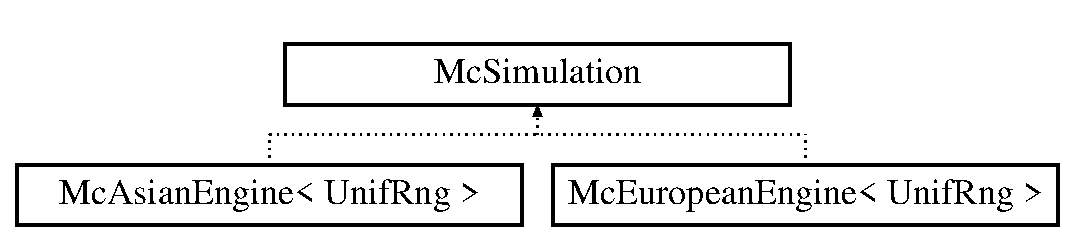
\includegraphics[height=2.000000cm]{class_mc_simulation}
\end{center}
\end{figure}
\subsection*{Public Member Functions}
\begin{DoxyCompactItemize}
\item 
\hypertarget{class_mc_simulation_a34949008df3c2b7fd4df32fac3875582}{}\label{class_mc_simulation_a34949008df3c2b7fd4df32fac3875582} 
void {\bfseries calculate} (unsigned long max\+Samples, unsigned long min\+Samples)
\item 
\hypertarget{class_mc_simulation_a5f74044189f64941f7fd3aaa4acc8e8e}{}\label{class_mc_simulation_a5f74044189f64941f7fd3aaa4acc8e8e} 
void {\bfseries value} (unsigned long max\+Samples, unsigned long min\+Samples)
\item 
\hypertarget{class_mc_simulation_af66197576bd23e26e91636f8ca1c7197}{}\label{class_mc_simulation_af66197576bd23e26e91636f8ca1c7197} 
const \hyperlink{class_m_c_statistics}{M\+C\+Statistics} \& {\bfseries sample\+Accumulator} () const
\end{DoxyCompactItemize}


The documentation for this class was generated from the following files\+:\begin{DoxyCompactItemize}
\item 
Users/\+C\+U\+I/\+Dropbox/\+C++/\+Finance/\+Mc\+Framework/Mc\+Simulation.\+h\item 
Users/\+C\+U\+I/\+Dropbox/\+C++/\+Finance/\+Mc\+Framework/Mc\+Simulation.\+cpp\end{DoxyCompactItemize}

\hypertarget{class_m_c_statistics}{}\section{M\+C\+Statistics Class Reference}
\label{class_m_c_statistics}\index{M\+C\+Statistics@{M\+C\+Statistics}}
\subsection*{Classes}
\begin{DoxyCompactItemize}
\item 
class \hyperlink{class_m_c_statistics_1_1_sample_results}{Sample\+Results}
\end{DoxyCompactItemize}
\subsection*{Public Member Functions}
\begin{DoxyCompactItemize}
\item 
\hypertarget{class_m_c_statistics_af1aab02cf590dee3fdc6d7b6cf9443fa}{}\label{class_m_c_statistics_af1aab02cf590dee3fdc6d7b6cf9443fa} 
Money {\bfseries mean} () const
\item 
\hypertarget{class_m_c_statistics_a6557ced886141997d13d86777b1970c5}{}\label{class_m_c_statistics_a6557ced886141997d13d86777b1970c5} 
void {\bfseries add} (unsigned long num\+Sample, Money price)
\end{DoxyCompactItemize}


The documentation for this class was generated from the following files\+:\begin{DoxyCompactItemize}
\item 
Users/\+C\+U\+I/\+Dropbox/\+C++/\+Finance/Statistics.\+h\item 
Users/\+C\+U\+I/\+Dropbox/\+C++/\+Finance/Statistics.\+cpp\end{DoxyCompactItemize}

\hypertarget{class_model}{}\section{Model Class Reference}
\label{class_model}\index{Model@{Model}}


{\ttfamily \#include $<$Model.\+h$>$}

Inheritance diagram for Model\+:\begin{figure}[H]
\begin{center}
\leavevmode
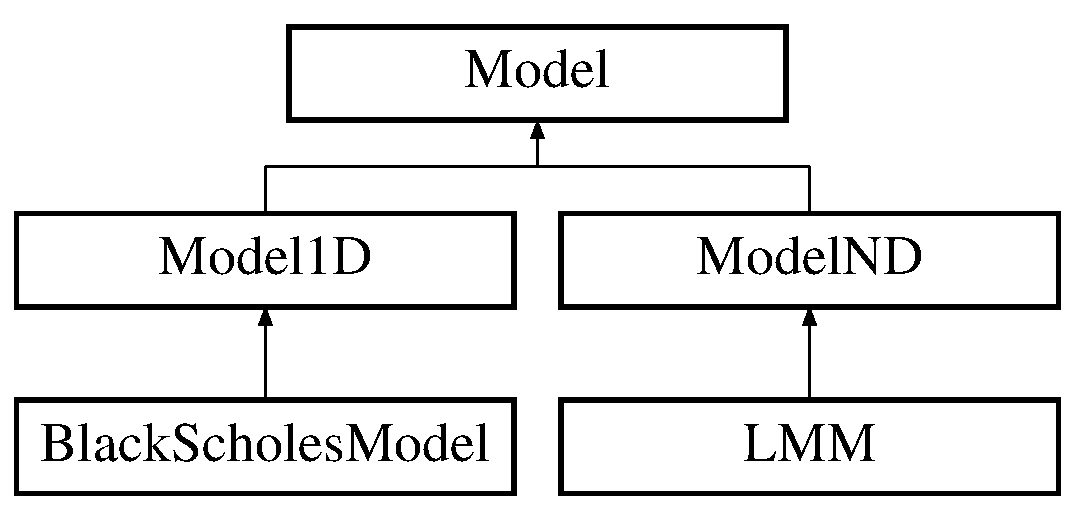
\includegraphics[height=3.000000cm]{class_model}
\end{center}
\end{figure}
\subsection*{Public Member Functions}
\begin{DoxyCompactItemize}
\item 
virtual std\+::vector$<$ \hyperlink{_name_def_8h_a642a6c5fd87319d922637de0e0bb0305}{Quote} $>$ \hyperlink{class_model_a087d56280bb51e8b04be3a9a30d06c76}{evolve} (\hyperlink{_name_def_8h_ac2d3e0ba793497bcca555c7c2cf64ff3}{Time} t0, std\+::vector$<$ \hyperlink{_name_def_8h_a642a6c5fd87319d922637de0e0bb0305}{Quote} $>$ \&x0, \hyperlink{_name_def_8h_ac2d3e0ba793497bcca555c7c2cf64ff3}{Time} dt, double dw) const =0
\item 
virtual const std\+::shared\+\_\+ptr$<$ \hyperlink{class_stochastic_process}{Stochastic\+Process} $>$ \& \hyperlink{class_model_adc6a695d3f6b2def79f2dde69b3ab547}{get\+Process} () const =0
\item 
virtual const std\+::shared\+\_\+ptr$<$ \hyperlink{class_stochastic_process}{Stochastic\+Process} $>$ \& \hyperlink{class_model_a23adaaf21b2955a1f4d4893ad9b77f02}{get\+Process} (int i) const =0
\item 
virtual unsigned long \hyperlink{class_model_acbe41cf30367bce4b96e92812d644f2d}{get\+Dimensionality} () const =0
\item 
const std\+::vector$<$ \hyperlink{_name_def_8h_a642a6c5fd87319d922637de0e0bb0305}{Quote} $>$ \& \hyperlink{class_model_ade5d08aae4d32777bfa048f356bbcca9}{get\+Initial} () const
\end{DoxyCompactItemize}
\subsection*{Protected Attributes}
\begin{DoxyCompactItemize}
\item 
std\+::vector$<$ \hyperlink{_name_def_8h_a642a6c5fd87319d922637de0e0bb0305}{Quote} $>$ \hyperlink{class_model_aea7cb62b50849b8c9beef1493435241e}{x0\+\_\+}
\end{DoxyCompactItemize}


\subsection{Member Function Documentation}
\hypertarget{class_model_a087d56280bb51e8b04be3a9a30d06c76}{}\label{class_model_a087d56280bb51e8b04be3a9a30d06c76} 
\index{Model@{Model}!evolve@{evolve}}
\index{evolve@{evolve}!Model@{Model}}
\subsubsection{\texorpdfstring{evolve()}{evolve()}}
{\footnotesize\ttfamily virtual std\+::vector$<$\hyperlink{_name_def_8h_a642a6c5fd87319d922637de0e0bb0305}{Quote}$>$ Model\+::evolve (\begin{DoxyParamCaption}\item[{\hyperlink{_name_def_8h_ac2d3e0ba793497bcca555c7c2cf64ff3}{Time}}]{t0,  }\item[{std\+::vector$<$ \hyperlink{_name_def_8h_a642a6c5fd87319d922637de0e0bb0305}{Quote} $>$ \&}]{x0,  }\item[{\hyperlink{_name_def_8h_ac2d3e0ba793497bcca555c7c2cf64ff3}{Time}}]{dt,  }\item[{double}]{dw }\end{DoxyParamCaption}) const\hspace{0.3cm}{\ttfamily [pure virtual]}}



Implemented in \hyperlink{class_l_m_m_a8dfdd340048e482a8059f473b5aacfd1}{L\+MM}, and \hyperlink{class_black_scholes_model_ae7ece51fd9f0eac3f77975cff857216d}{Black\+Scholes\+Model}.

\hypertarget{class_model_acbe41cf30367bce4b96e92812d644f2d}{}\label{class_model_acbe41cf30367bce4b96e92812d644f2d} 
\index{Model@{Model}!get\+Dimensionality@{get\+Dimensionality}}
\index{get\+Dimensionality@{get\+Dimensionality}!Model@{Model}}
\subsubsection{\texorpdfstring{get\+Dimensionality()}{getDimensionality()}}
{\footnotesize\ttfamily virtual unsigned long Model\+::get\+Dimensionality (\begin{DoxyParamCaption}{ }\end{DoxyParamCaption}) const\hspace{0.3cm}{\ttfamily [pure virtual]}}



Implemented in \hyperlink{class_model_n_d_ab2356536a38f4961257654de629d6093}{Model\+ND}, and \hyperlink{class_model1_d_ac81875523be6153cb58d0f37914eb9a1}{Model1D}.

\hypertarget{class_model_ade5d08aae4d32777bfa048f356bbcca9}{}\label{class_model_ade5d08aae4d32777bfa048f356bbcca9} 
\index{Model@{Model}!get\+Initial@{get\+Initial}}
\index{get\+Initial@{get\+Initial}!Model@{Model}}
\subsubsection{\texorpdfstring{get\+Initial()}{getInitial()}}
{\footnotesize\ttfamily const std\+::vector$<$\hyperlink{_name_def_8h_a642a6c5fd87319d922637de0e0bb0305}{Quote}$>$\& Model\+::get\+Initial (\begin{DoxyParamCaption}{ }\end{DoxyParamCaption}) const\hspace{0.3cm}{\ttfamily [inline]}}

\hypertarget{class_model_adc6a695d3f6b2def79f2dde69b3ab547}{}\label{class_model_adc6a695d3f6b2def79f2dde69b3ab547} 
\index{Model@{Model}!get\+Process@{get\+Process}}
\index{get\+Process@{get\+Process}!Model@{Model}}
\subsubsection{\texorpdfstring{get\+Process()}{getProcess()}\hspace{0.1cm}{\footnotesize\ttfamily [1/2]}}
{\footnotesize\ttfamily virtual const std\+::shared\+\_\+ptr$<$\hyperlink{class_stochastic_process}{Stochastic\+Process}$>$\& Model\+::get\+Process (\begin{DoxyParamCaption}{ }\end{DoxyParamCaption}) const\hspace{0.3cm}{\ttfamily [pure virtual]}}



Implemented in \hyperlink{class_model_n_d_a98976fe73a8895ff98ba60ea174232f8}{Model\+ND}, and \hyperlink{class_model1_d_ae3cdfcb2922f03a68b8e8e02d572746f}{Model1D}.

\hypertarget{class_model_a23adaaf21b2955a1f4d4893ad9b77f02}{}\label{class_model_a23adaaf21b2955a1f4d4893ad9b77f02} 
\index{Model@{Model}!get\+Process@{get\+Process}}
\index{get\+Process@{get\+Process}!Model@{Model}}
\subsubsection{\texorpdfstring{get\+Process()}{getProcess()}\hspace{0.1cm}{\footnotesize\ttfamily [2/2]}}
{\footnotesize\ttfamily virtual const std\+::shared\+\_\+ptr$<$\hyperlink{class_stochastic_process}{Stochastic\+Process}$>$\& Model\+::get\+Process (\begin{DoxyParamCaption}\item[{int}]{i }\end{DoxyParamCaption}) const\hspace{0.3cm}{\ttfamily [pure virtual]}}



Implemented in \hyperlink{class_model_n_d_a62866814432b7c0a0d8f58223cc6279d}{Model\+ND}, and \hyperlink{class_model1_d_a08b3a9f594214b5e3bcba3fe5f63524e}{Model1D}.



\subsection{Member Data Documentation}
\hypertarget{class_model_aea7cb62b50849b8c9beef1493435241e}{}\label{class_model_aea7cb62b50849b8c9beef1493435241e} 
\index{Model@{Model}!x0\+\_\+@{x0\+\_\+}}
\index{x0\+\_\+@{x0\+\_\+}!Model@{Model}}
\subsubsection{\texorpdfstring{x0\+\_\+}{x0\_}}
{\footnotesize\ttfamily std\+::vector$<$\hyperlink{_name_def_8h_a642a6c5fd87319d922637de0e0bb0305}{Quote}$>$ Model\+::x0\+\_\+\hspace{0.3cm}{\ttfamily [mutable]}, {\ttfamily [protected]}}



The documentation for this class was generated from the following file\+:\begin{DoxyCompactItemize}
\item 
Users/\+C\+U\+I/\+Dropbox/\+C++/\+Finance/\hyperlink{_model_8h}{Model.\+h}\end{DoxyCompactItemize}

\hypertarget{class_model1_d}{}\section{Model1D Class Reference}
\label{class_model1_d}\index{Model1D@{Model1D}}


{\ttfamily \#include $<$Model.\+h$>$}

Inheritance diagram for Model1D\+:\begin{figure}[H]
\begin{center}
\leavevmode
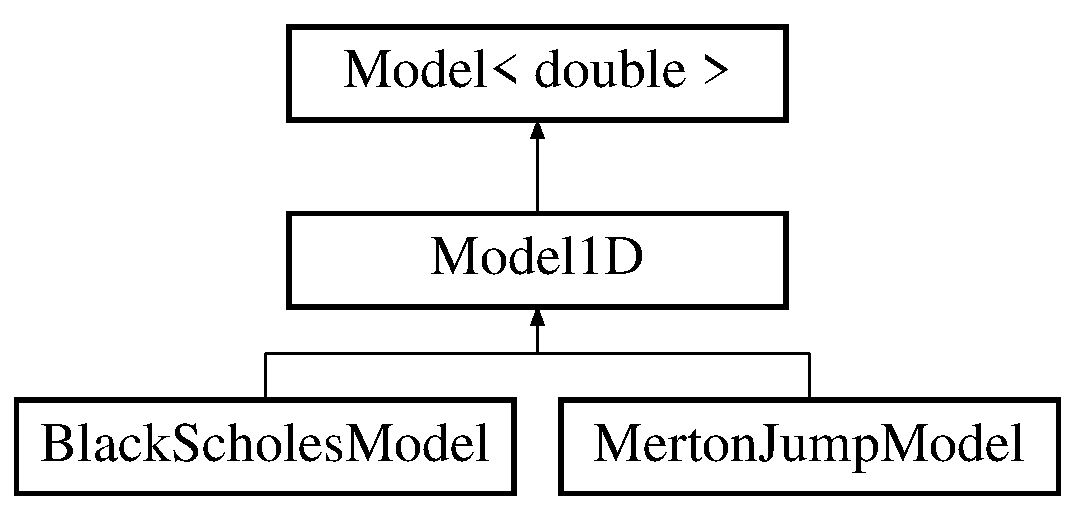
\includegraphics[height=3.000000cm]{class_model1_d}
\end{center}
\end{figure}
\subsection*{Public Member Functions}
\begin{DoxyCompactItemize}
\item 
\hyperlink{class_model1_d_a4a4fa285bc474bd52d8a9bc1bc4f2dbf}{Model1D} ()=default
\item 
\hyperlink{class_model1_d_a0dcf861b2408b4254fb0176ef99e320c}{Model1D} (const shared\+\_\+ptr$<$ \hyperlink{class_stochastic_process}{Stochastic\+Process} $>$ \&process)
\item 
const shared\+\_\+ptr$<$ \hyperlink{class_stochastic_process}{Stochastic\+Process} $>$ \& \hyperlink{class_model1_d_a670fd7ee0b66d5d865e0d13d6e50bb40}{get\+Process} () const override
\item 
const shared\+\_\+ptr$<$ \hyperlink{class_stochastic_process}{Stochastic\+Process} $>$ \& \hyperlink{class_model1_d_af7ff938fd134829e876c41fc8be8c24f}{get\+Process} (int i) const override
\item 
unsigned long \hyperlink{class_model1_d_ac81875523be6153cb58d0f37914eb9a1}{get\+Dimensionality} () const override
\item 
void \hyperlink{class_model1_d_ab6c3618666b21f261898597e6e416495}{set\+Model} (const shared\+\_\+ptr$<$ \hyperlink{class_stochastic_process}{Stochastic\+Process} $>$ \&process)
\end{DoxyCompactItemize}
\subsection*{Protected Attributes}
\begin{DoxyCompactItemize}
\item 
shared\+\_\+ptr$<$ \hyperlink{class_stochastic_process}{Stochastic\+Process} $>$ \hyperlink{class_model1_d_af3ea570fe242020bab49cc9530c6bd98}{process\+\_\+}
\end{DoxyCompactItemize}


\subsection{Constructor \& Destructor Documentation}
\hypertarget{class_model1_d_a4a4fa285bc474bd52d8a9bc1bc4f2dbf}{}\label{class_model1_d_a4a4fa285bc474bd52d8a9bc1bc4f2dbf} 
\index{Model1D@{Model1D}!Model1D@{Model1D}}
\index{Model1D@{Model1D}!Model1D@{Model1D}}
\subsubsection{\texorpdfstring{Model1\+D()}{Model1D()}\hspace{0.1cm}{\footnotesize\ttfamily [1/2]}}
{\footnotesize\ttfamily Model1\+D\+::\+Model1D (\begin{DoxyParamCaption}{ }\end{DoxyParamCaption})\hspace{0.3cm}{\ttfamily [default]}}

\hypertarget{class_model1_d_a0dcf861b2408b4254fb0176ef99e320c}{}\label{class_model1_d_a0dcf861b2408b4254fb0176ef99e320c} 
\index{Model1D@{Model1D}!Model1D@{Model1D}}
\index{Model1D@{Model1D}!Model1D@{Model1D}}
\subsubsection{\texorpdfstring{Model1\+D()}{Model1D()}\hspace{0.1cm}{\footnotesize\ttfamily [2/2]}}
{\footnotesize\ttfamily Model1\+D\+::\+Model1D (\begin{DoxyParamCaption}\item[{const shared\+\_\+ptr$<$ \hyperlink{class_stochastic_process}{Stochastic\+Process} $>$ \&}]{process }\end{DoxyParamCaption})\hspace{0.3cm}{\ttfamily [inline]}}



\subsection{Member Function Documentation}
\hypertarget{class_model1_d_ac81875523be6153cb58d0f37914eb9a1}{}\label{class_model1_d_ac81875523be6153cb58d0f37914eb9a1} 
\index{Model1D@{Model1D}!get\+Dimensionality@{get\+Dimensionality}}
\index{get\+Dimensionality@{get\+Dimensionality}!Model1D@{Model1D}}
\subsubsection{\texorpdfstring{get\+Dimensionality()}{getDimensionality()}}
{\footnotesize\ttfamily unsigned long Model1\+D\+::get\+Dimensionality (\begin{DoxyParamCaption}{ }\end{DoxyParamCaption}) const\hspace{0.3cm}{\ttfamily [inline]}, {\ttfamily [override]}, {\ttfamily [virtual]}}



Implements \hyperlink{class_model_a26832ec2df24d7941783d3cd6d500898}{Model$<$ double $>$}.

\hypertarget{class_model1_d_a670fd7ee0b66d5d865e0d13d6e50bb40}{}\label{class_model1_d_a670fd7ee0b66d5d865e0d13d6e50bb40} 
\index{Model1D@{Model1D}!get\+Process@{get\+Process}}
\index{get\+Process@{get\+Process}!Model1D@{Model1D}}
\subsubsection{\texorpdfstring{get\+Process()}{getProcess()}\hspace{0.1cm}{\footnotesize\ttfamily [1/2]}}
{\footnotesize\ttfamily const shared\+\_\+ptr$<$\hyperlink{class_stochastic_process}{Stochastic\+Process}$>$\& Model1\+D\+::get\+Process (\begin{DoxyParamCaption}{ }\end{DoxyParamCaption}) const\hspace{0.3cm}{\ttfamily [inline]}, {\ttfamily [override]}, {\ttfamily [virtual]}}



Implements \hyperlink{class_model_a6f584114ffcbd4eac04a2bbf8e9cede2}{Model$<$ double $>$}.

\hypertarget{class_model1_d_af7ff938fd134829e876c41fc8be8c24f}{}\label{class_model1_d_af7ff938fd134829e876c41fc8be8c24f} 
\index{Model1D@{Model1D}!get\+Process@{get\+Process}}
\index{get\+Process@{get\+Process}!Model1D@{Model1D}}
\subsubsection{\texorpdfstring{get\+Process()}{getProcess()}\hspace{0.1cm}{\footnotesize\ttfamily [2/2]}}
{\footnotesize\ttfamily const shared\+\_\+ptr$<$\hyperlink{class_stochastic_process}{Stochastic\+Process}$>$\& Model1\+D\+::get\+Process (\begin{DoxyParamCaption}\item[{int}]{i }\end{DoxyParamCaption}) const\hspace{0.3cm}{\ttfamily [inline]}, {\ttfamily [override]}, {\ttfamily [virtual]}}



Implements \hyperlink{class_model_a7b9e58a51a5d244aa7012f1cdb7aebd8}{Model$<$ double $>$}.

\hypertarget{class_model1_d_ab6c3618666b21f261898597e6e416495}{}\label{class_model1_d_ab6c3618666b21f261898597e6e416495} 
\index{Model1D@{Model1D}!set\+Model@{set\+Model}}
\index{set\+Model@{set\+Model}!Model1D@{Model1D}}
\subsubsection{\texorpdfstring{set\+Model()}{setModel()}}
{\footnotesize\ttfamily void Model1\+D\+::set\+Model (\begin{DoxyParamCaption}\item[{const shared\+\_\+ptr$<$ \hyperlink{class_stochastic_process}{Stochastic\+Process} $>$ \&}]{process }\end{DoxyParamCaption})\hspace{0.3cm}{\ttfamily [inline]}}



\subsection{Member Data Documentation}
\hypertarget{class_model1_d_af3ea570fe242020bab49cc9530c6bd98}{}\label{class_model1_d_af3ea570fe242020bab49cc9530c6bd98} 
\index{Model1D@{Model1D}!process\+\_\+@{process\+\_\+}}
\index{process\+\_\+@{process\+\_\+}!Model1D@{Model1D}}
\subsubsection{\texorpdfstring{process\+\_\+}{process\_}}
{\footnotesize\ttfamily shared\+\_\+ptr$<$\hyperlink{class_stochastic_process}{Stochastic\+Process}$>$ Model1\+D\+::process\+\_\+\hspace{0.3cm}{\ttfamily [protected]}}



The documentation for this class was generated from the following file\+:\begin{DoxyCompactItemize}
\item 
\hyperlink{_model_8h}{Model.\+h}\end{DoxyCompactItemize}

\hypertarget{class_model_n_d}{}\section{Model\+ND Class Reference}
\label{class_model_n_d}\index{Model\+ND@{Model\+ND}}


{\ttfamily \#include $<$Model.\+h$>$}

Inheritance diagram for Model\+ND\+:\begin{figure}[H]
\begin{center}
\leavevmode
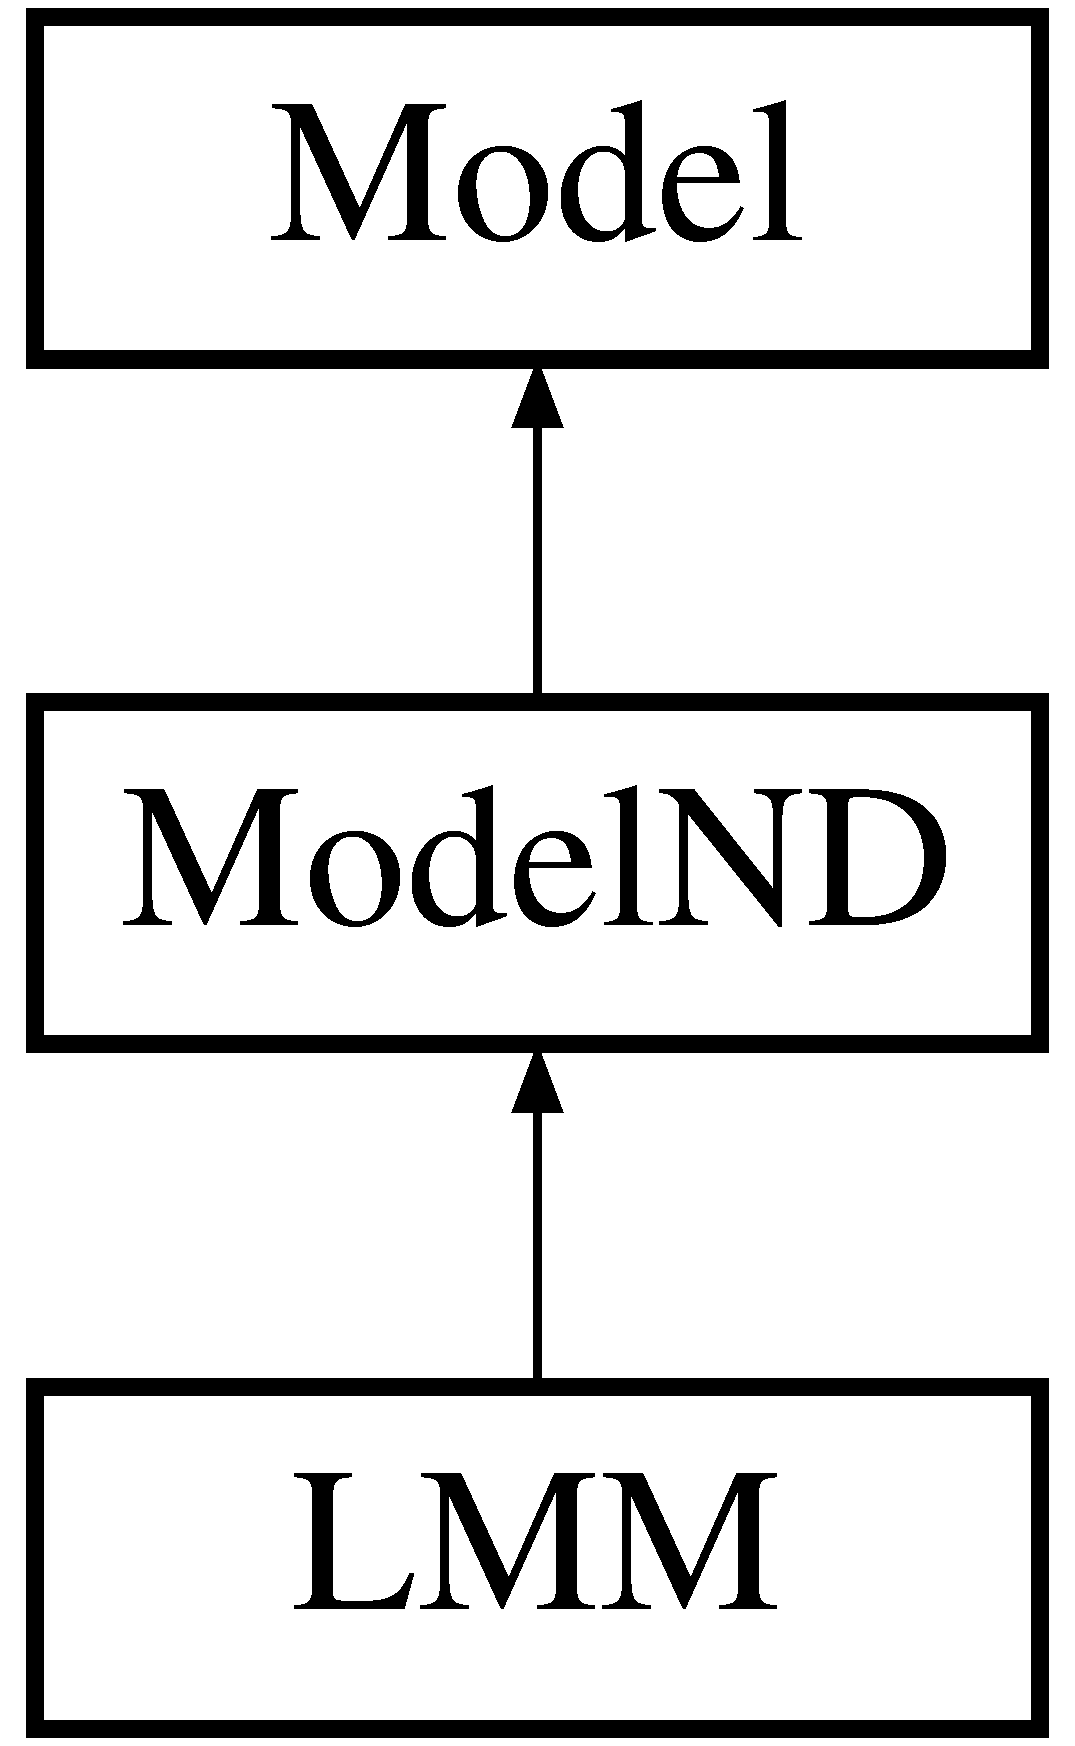
\includegraphics[height=3.000000cm]{class_model_n_d}
\end{center}
\end{figure}
\subsection*{Public Member Functions}
\begin{DoxyCompactItemize}
\item 
const std\+::shared\+\_\+ptr$<$ \hyperlink{class_stochastic_process}{Stochastic\+Process} $>$ \& \hyperlink{class_model_n_d_a98976fe73a8895ff98ba60ea174232f8}{get\+Process} () const override
\item 
const std\+::shared\+\_\+ptr$<$ \hyperlink{class_stochastic_process}{Stochastic\+Process} $>$ \& \hyperlink{class_model_n_d_a62866814432b7c0a0d8f58223cc6279d}{get\+Process} (int i) const override
\item 
unsigned long \hyperlink{class_model_n_d_ab2356536a38f4961257654de629d6093}{get\+Dimensionality} () const override
\end{DoxyCompactItemize}
\subsection*{Protected Attributes}
\begin{DoxyCompactItemize}
\item 
std\+::vector$<$ std\+::shared\+\_\+ptr$<$ \hyperlink{class_stochastic_process}{Stochastic\+Process} $>$ $>$ \hyperlink{class_model_n_d_a9cb778073c54caae0ffea17a59a9a2f9}{processes\+\_\+}
\item 
unsigned long \hyperlink{class_model_n_d_ac86872437daeeffeb8fb1b387bea28f8}{dimension\+\_\+}
\end{DoxyCompactItemize}


\subsection{Member Function Documentation}
\hypertarget{class_model_n_d_ab2356536a38f4961257654de629d6093}{}\label{class_model_n_d_ab2356536a38f4961257654de629d6093} 
\index{Model\+ND@{Model\+ND}!get\+Dimensionality@{get\+Dimensionality}}
\index{get\+Dimensionality@{get\+Dimensionality}!Model\+ND@{Model\+ND}}
\subsubsection{\texorpdfstring{get\+Dimensionality()}{getDimensionality()}}
{\footnotesize\ttfamily unsigned long Model\+N\+D\+::get\+Dimensionality (\begin{DoxyParamCaption}{ }\end{DoxyParamCaption}) const\hspace{0.3cm}{\ttfamily [inline]}, {\ttfamily [override]}, {\ttfamily [virtual]}}



Implements \hyperlink{class_model_acbe41cf30367bce4b96e92812d644f2d}{Model}.

\hypertarget{class_model_n_d_a98976fe73a8895ff98ba60ea174232f8}{}\label{class_model_n_d_a98976fe73a8895ff98ba60ea174232f8} 
\index{Model\+ND@{Model\+ND}!get\+Process@{get\+Process}}
\index{get\+Process@{get\+Process}!Model\+ND@{Model\+ND}}
\subsubsection{\texorpdfstring{get\+Process()}{getProcess()}\hspace{0.1cm}{\footnotesize\ttfamily [1/2]}}
{\footnotesize\ttfamily const std\+::shared\+\_\+ptr$<$\hyperlink{class_stochastic_process}{Stochastic\+Process}$>$\& Model\+N\+D\+::get\+Process (\begin{DoxyParamCaption}{ }\end{DoxyParamCaption}) const\hspace{0.3cm}{\ttfamily [inline]}, {\ttfamily [override]}, {\ttfamily [virtual]}}



Implements \hyperlink{class_model_adc6a695d3f6b2def79f2dde69b3ab547}{Model}.

\hypertarget{class_model_n_d_a62866814432b7c0a0d8f58223cc6279d}{}\label{class_model_n_d_a62866814432b7c0a0d8f58223cc6279d} 
\index{Model\+ND@{Model\+ND}!get\+Process@{get\+Process}}
\index{get\+Process@{get\+Process}!Model\+ND@{Model\+ND}}
\subsubsection{\texorpdfstring{get\+Process()}{getProcess()}\hspace{0.1cm}{\footnotesize\ttfamily [2/2]}}
{\footnotesize\ttfamily const std\+::shared\+\_\+ptr$<$\hyperlink{class_stochastic_process}{Stochastic\+Process}$>$\& Model\+N\+D\+::get\+Process (\begin{DoxyParamCaption}\item[{int}]{i }\end{DoxyParamCaption}) const\hspace{0.3cm}{\ttfamily [inline]}, {\ttfamily [override]}, {\ttfamily [virtual]}}



Implements \hyperlink{class_model_a23adaaf21b2955a1f4d4893ad9b77f02}{Model}.



\subsection{Member Data Documentation}
\hypertarget{class_model_n_d_ac86872437daeeffeb8fb1b387bea28f8}{}\label{class_model_n_d_ac86872437daeeffeb8fb1b387bea28f8} 
\index{Model\+ND@{Model\+ND}!dimension\+\_\+@{dimension\+\_\+}}
\index{dimension\+\_\+@{dimension\+\_\+}!Model\+ND@{Model\+ND}}
\subsubsection{\texorpdfstring{dimension\+\_\+}{dimension\_}}
{\footnotesize\ttfamily unsigned long Model\+N\+D\+::dimension\+\_\+\hspace{0.3cm}{\ttfamily [protected]}}

\hypertarget{class_model_n_d_a9cb778073c54caae0ffea17a59a9a2f9}{}\label{class_model_n_d_a9cb778073c54caae0ffea17a59a9a2f9} 
\index{Model\+ND@{Model\+ND}!processes\+\_\+@{processes\+\_\+}}
\index{processes\+\_\+@{processes\+\_\+}!Model\+ND@{Model\+ND}}
\subsubsection{\texorpdfstring{processes\+\_\+}{processes\_}}
{\footnotesize\ttfamily std\+::vector$<$std\+::shared\+\_\+ptr$<$\hyperlink{class_stochastic_process}{Stochastic\+Process}$>$ $>$ Model\+N\+D\+::processes\+\_\+\hspace{0.3cm}{\ttfamily [protected]}}



The documentation for this class was generated from the following file\+:\begin{DoxyCompactItemize}
\item 
\hyperlink{_model_8h}{Model.\+h}\end{DoxyCompactItemize}

\hypertarget{class_normal_marsaglia_bray_rng}{}\section{Normal\+Marsaglia\+Bray\+Rng$<$ Uniform\+R\+NG $>$ Class Template Reference}
\label{class_normal_marsaglia_bray_rng}\index{Normal\+Marsaglia\+Bray\+Rng$<$ Uniform\+R\+N\+G $>$@{Normal\+Marsaglia\+Bray\+Rng$<$ Uniform\+R\+N\+G $>$}}
\subsection*{Public Member Functions}
\begin{DoxyCompactItemize}
\item 
\hypertarget{class_normal_marsaglia_bray_rng_a2cc54f5f331a5bd71eedc67c84db7279}{}\label{class_normal_marsaglia_bray_rng_a2cc54f5f331a5bd71eedc67c84db7279} 
double {\bfseries next} ()
\end{DoxyCompactItemize}


The documentation for this class was generated from the following file\+:\begin{DoxyCompactItemize}
\item 
Users/\+C\+U\+I/\+Dropbox/\+C++/\+Finance/\+Rand\+Num\+Generation/Normal\+Marsaglia\+Bray\+Rng.\+h\end{DoxyCompactItemize}

\hypertarget{class_null_parameter}{}\section{Null\+Parameter Class Reference}
\label{class_null_parameter}\index{Null\+Parameter@{Null\+Parameter}}


{\ttfamily \#include $<$Parameter.\+h$>$}

Inheritance diagram for Null\+Parameter\+:\begin{figure}[H]
\begin{center}
\leavevmode
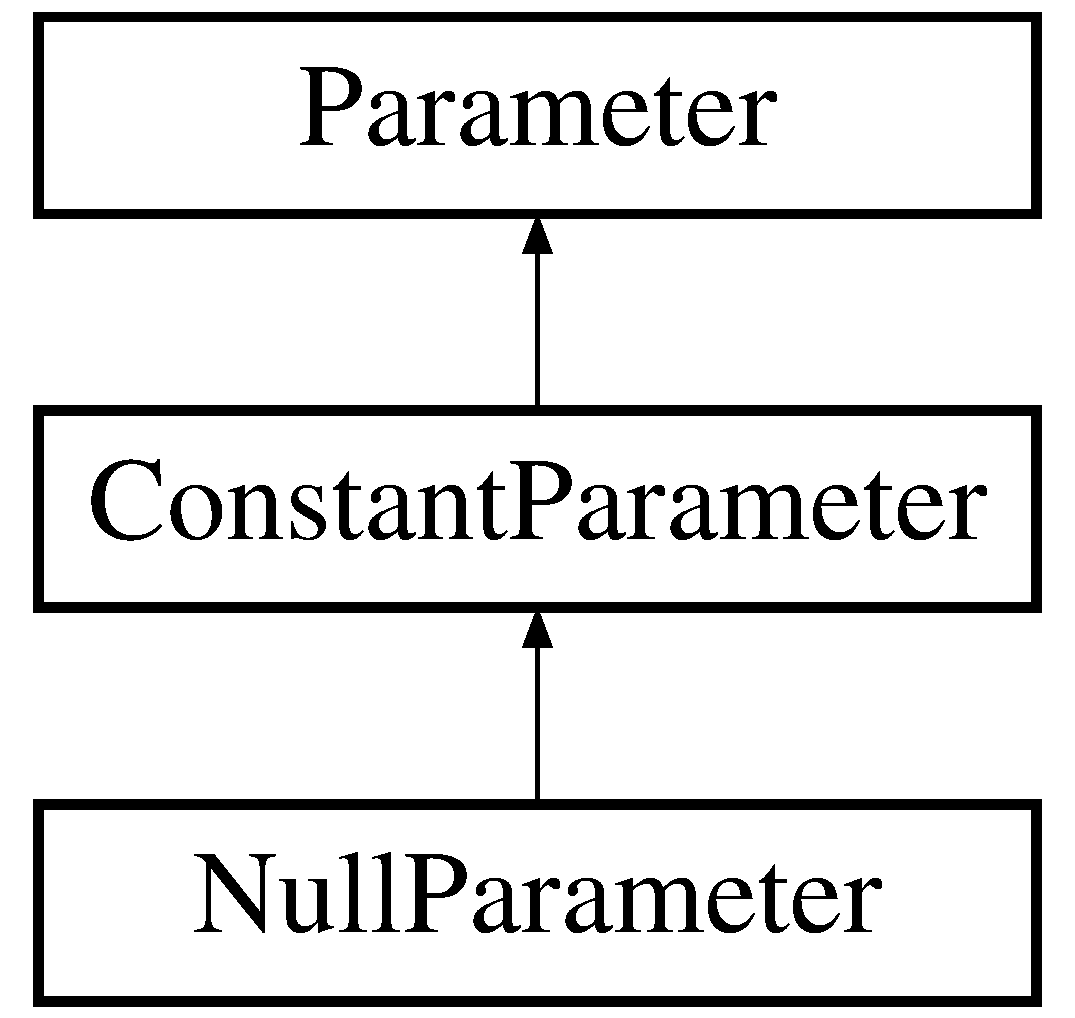
\includegraphics[height=3.000000cm]{class_null_parameter}
\end{center}
\end{figure}
\subsection*{Public Member Functions}
\begin{DoxyCompactItemize}
\item 
\hyperlink{class_null_parameter_aa11a91b9c36438288e91fbc3613bcda7}{Null\+Parameter} ()
\end{DoxyCompactItemize}
\subsection*{Additional Inherited Members}


\subsection{Constructor \& Destructor Documentation}
\hypertarget{class_null_parameter_aa11a91b9c36438288e91fbc3613bcda7}{}\label{class_null_parameter_aa11a91b9c36438288e91fbc3613bcda7} 
\index{Null\+Parameter@{Null\+Parameter}!Null\+Parameter@{Null\+Parameter}}
\index{Null\+Parameter@{Null\+Parameter}!Null\+Parameter@{Null\+Parameter}}
\subsubsection{\texorpdfstring{Null\+Parameter()}{NullParameter()}}
{\footnotesize\ttfamily Null\+Parameter\+::\+Null\+Parameter (\begin{DoxyParamCaption}{ }\end{DoxyParamCaption})\hspace{0.3cm}{\ttfamily [inline]}}



The documentation for this class was generated from the following file\+:\begin{DoxyCompactItemize}
\item 
\hyperlink{_parameter_8h}{Parameter.\+h}\end{DoxyCompactItemize}

\hypertarget{class_parameter}{}\section{Parameter Class Reference}
\label{class_parameter}\index{Parameter@{Parameter}}


{\ttfamily \#include $<$Parameter.\+h$>$}

Inheritance diagram for Parameter\+:\begin{figure}[H]
\begin{center}
\leavevmode
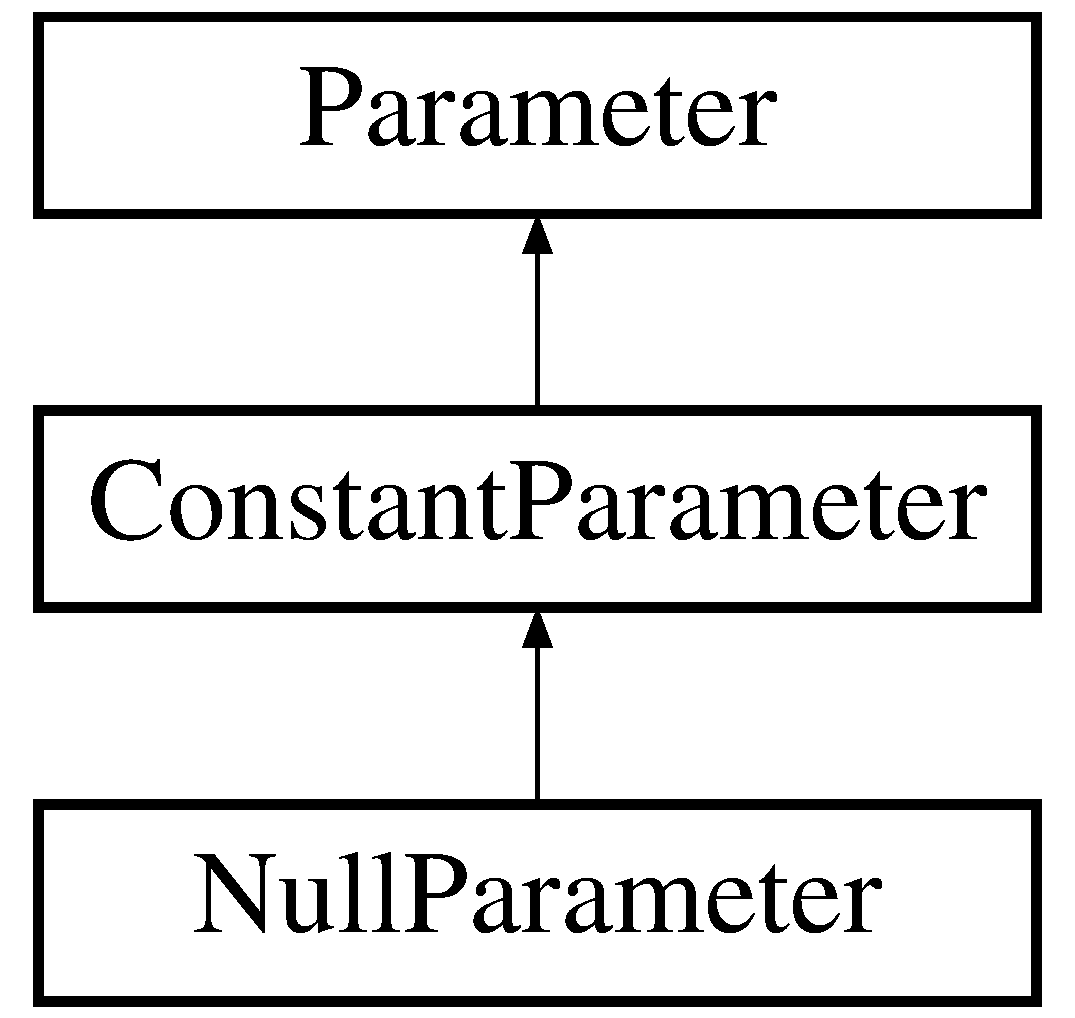
\includegraphics[height=3.000000cm]{class_parameter}
\end{center}
\end{figure}
\subsection*{Public Member Functions}
\begin{DoxyCompactItemize}
\item 
\hyperlink{class_parameter_a5de1d76f6b0342f3e98d004733ce9c2c}{Parameter} ()=default
\item 
\hyperlink{class_parameter_a07b46a4af924cbaea806505343d7b83a}{Parameter} (const \hyperlink{class_parameter}{Parameter} \&)=default
\item 
\hyperlink{class_parameter}{Parameter} \& \hyperlink{class_parameter_ac7e34f069ed1474901fce2f06e0ee54f}{operator=} (const \hyperlink{class_parameter}{Parameter} \&)=default
\item 
virtual double \hyperlink{class_parameter_ae6317fac3d0b5e69101eb7059d151ca7}{operator()} (\hyperlink{_name_def_8h_ac2d3e0ba793497bcca555c7c2cf64ff3}{Time} t) const =0
\item 
void \hyperlink{class_parameter_a8cebb26e89537b098c8b42ef9aeb0f66}{set\+Param} (int i, double new\+Val)
\item 
unsigned long \hyperlink{class_parameter_ae1ca6e3ab5f2d2ed3bffbdee6e941068}{size} () const
\end{DoxyCompactItemize}
\subsection*{Protected Attributes}
\begin{DoxyCompactItemize}
\item 
vector$<$ double $>$ \hyperlink{class_parameter_ab7e9f6b7b261380449ff0eca797e48e7}{params\+\_\+}
\end{DoxyCompactItemize}


\subsection{Constructor \& Destructor Documentation}
\hypertarget{class_parameter_a5de1d76f6b0342f3e98d004733ce9c2c}{}\label{class_parameter_a5de1d76f6b0342f3e98d004733ce9c2c} 
\index{Parameter@{Parameter}!Parameter@{Parameter}}
\index{Parameter@{Parameter}!Parameter@{Parameter}}
\subsubsection{\texorpdfstring{Parameter()}{Parameter()}\hspace{0.1cm}{\footnotesize\ttfamily [1/2]}}
{\footnotesize\ttfamily Parameter\+::\+Parameter (\begin{DoxyParamCaption}{ }\end{DoxyParamCaption})\hspace{0.3cm}{\ttfamily [default]}}

\hypertarget{class_parameter_a07b46a4af924cbaea806505343d7b83a}{}\label{class_parameter_a07b46a4af924cbaea806505343d7b83a} 
\index{Parameter@{Parameter}!Parameter@{Parameter}}
\index{Parameter@{Parameter}!Parameter@{Parameter}}
\subsubsection{\texorpdfstring{Parameter()}{Parameter()}\hspace{0.1cm}{\footnotesize\ttfamily [2/2]}}
{\footnotesize\ttfamily Parameter\+::\+Parameter (\begin{DoxyParamCaption}\item[{const \hyperlink{class_parameter}{Parameter} \&}]{ }\end{DoxyParamCaption})\hspace{0.3cm}{\ttfamily [default]}}



\subsection{Member Function Documentation}
\hypertarget{class_parameter_ae6317fac3d0b5e69101eb7059d151ca7}{}\label{class_parameter_ae6317fac3d0b5e69101eb7059d151ca7} 
\index{Parameter@{Parameter}!operator()@{operator()}}
\index{operator()@{operator()}!Parameter@{Parameter}}
\subsubsection{\texorpdfstring{operator()()}{operator()()}}
{\footnotesize\ttfamily virtual double Parameter\+::operator() (\begin{DoxyParamCaption}\item[{\hyperlink{_name_def_8h_ac2d3e0ba793497bcca555c7c2cf64ff3}{Time}}]{t }\end{DoxyParamCaption}) const\hspace{0.3cm}{\ttfamily [pure virtual]}}



Implemented in \hyperlink{class_constant_parameter_a23abb141692843e2ef68d43f610beb5e}{Constant\+Parameter}.

\hypertarget{class_parameter_ac7e34f069ed1474901fce2f06e0ee54f}{}\label{class_parameter_ac7e34f069ed1474901fce2f06e0ee54f} 
\index{Parameter@{Parameter}!operator=@{operator=}}
\index{operator=@{operator=}!Parameter@{Parameter}}
\subsubsection{\texorpdfstring{operator=()}{operator=()}}
{\footnotesize\ttfamily \hyperlink{class_parameter}{Parameter}\& Parameter\+::operator= (\begin{DoxyParamCaption}\item[{const \hyperlink{class_parameter}{Parameter} \&}]{ }\end{DoxyParamCaption})\hspace{0.3cm}{\ttfamily [default]}}

\hypertarget{class_parameter_a8cebb26e89537b098c8b42ef9aeb0f66}{}\label{class_parameter_a8cebb26e89537b098c8b42ef9aeb0f66} 
\index{Parameter@{Parameter}!set\+Param@{set\+Param}}
\index{set\+Param@{set\+Param}!Parameter@{Parameter}}
\subsubsection{\texorpdfstring{set\+Param()}{setParam()}}
{\footnotesize\ttfamily void Parameter\+::set\+Param (\begin{DoxyParamCaption}\item[{int}]{i,  }\item[{double}]{new\+Val }\end{DoxyParamCaption})\hspace{0.3cm}{\ttfamily [inline]}}

\hypertarget{class_parameter_ae1ca6e3ab5f2d2ed3bffbdee6e941068}{}\label{class_parameter_ae1ca6e3ab5f2d2ed3bffbdee6e941068} 
\index{Parameter@{Parameter}!size@{size}}
\index{size@{size}!Parameter@{Parameter}}
\subsubsection{\texorpdfstring{size()}{size()}}
{\footnotesize\ttfamily unsigned long Parameter\+::size (\begin{DoxyParamCaption}{ }\end{DoxyParamCaption}) const\hspace{0.3cm}{\ttfamily [inline]}}



\subsection{Member Data Documentation}
\hypertarget{class_parameter_ab7e9f6b7b261380449ff0eca797e48e7}{}\label{class_parameter_ab7e9f6b7b261380449ff0eca797e48e7} 
\index{Parameter@{Parameter}!params\+\_\+@{params\+\_\+}}
\index{params\+\_\+@{params\+\_\+}!Parameter@{Parameter}}
\subsubsection{\texorpdfstring{params\+\_\+}{params\_}}
{\footnotesize\ttfamily vector$<$double$>$ Parameter\+::params\+\_\+\hspace{0.3cm}{\ttfamily [protected]}}



The documentation for this class was generated from the following file\+:\begin{DoxyCompactItemize}
\item 
\hyperlink{_parameter_8h}{Parameter.\+h}\end{DoxyCompactItemize}

\hypertarget{class_stochastic_process_1_1_parameter_set}{}\section{Stochastic\+Process\+:\+:Parameter\+Set Class Reference}
\label{class_stochastic_process_1_1_parameter_set}\index{Stochastic\+Process\+::\+Parameter\+Set@{Stochastic\+Process\+::\+Parameter\+Set}}


{\ttfamily \#include $<$Stochastic\+Process.\+h$>$}



The documentation for this class was generated from the following file\+:\begin{DoxyCompactItemize}
\item 
\hyperlink{_stochastic_process_8h}{Stochastic\+Process.\+h}\end{DoxyCompactItemize}

\hypertarget{class_path}{}\section{Path$<$ Path\+Type $>$ Class Template Reference}
\label{class_path}\index{Path$<$ Path\+Type $>$@{Path$<$ Path\+Type $>$}}


Base class for a single path.  




{\ttfamily \#include $<$Path.\+h$>$}

\subsection*{Public Types}
\begin{DoxyCompactItemize}
\item 
typedef Path\+Type\+::path\+\_\+return\+\_\+type \hyperlink{class_path_a3b1c34a87f7867f6fed2e0a33f801e7d}{path\+\_\+return\+\_\+type}
\begin{DoxyCompactList}\small\item\em Type of single path for Path\+Type. \end{DoxyCompactList}\end{DoxyCompactItemize}
\subsection*{Public Member Functions}
\begin{DoxyCompactItemize}
\item 
\hyperlink{class_path_ab0fff5e8514331bba55ab5745fc485a4}{Path} (const vector$<$ \hyperlink{_name_def_8h_ac2d3e0ba793497bcca555c7c2cf64ff3}{Time} $>$ \&time\+Grid, unsigned long dimension)
\begin{DoxyCompactList}\small\item\em Constructor. \end{DoxyCompactList}\item 
\hyperlink{class_path_a8437fecb95fe145057c957feb8b8955a}{Path} ()=default
\item 
virtual const vector$<$ \hyperlink{_name_def_8h_ac2d3e0ba793497bcca555c7c2cf64ff3}{Time} $>$ \& \hyperlink{class_path_a511b7a93c62893bcafba4749ad1dd1b3}{get\+Time\+Grid} () const
\begin{DoxyCompactList}\small\item\em Return the vector of time grid. \end{DoxyCompactList}\item 
virtual \hyperlink{class_path_a3b1c34a87f7867f6fed2e0a33f801e7d}{path\+\_\+return\+\_\+type} \& \hyperlink{class_path_a8ba07fadae45801824240317c311bb84}{get\+Values} ()
\begin{DoxyCompactList}\small\item\em Return the values of path. \end{DoxyCompactList}\item 
virtual const \hyperlink{class_path_a3b1c34a87f7867f6fed2e0a33f801e7d}{path\+\_\+return\+\_\+type} \& \hyperlink{class_path_a2490ad69198170463f98c7d8f7212917}{get\+Values} () const
\begin{DoxyCompactList}\small\item\em Return the values of path. \end{DoxyCompactList}\item 
virtual \hyperlink{class_path_a83933167b70441af12427b23d88b0447}{$\sim$\+Path} ()
\end{DoxyCompactItemize}
\subsection*{Private Attributes}
\begin{DoxyCompactItemize}
\item 
vector$<$ \hyperlink{_name_def_8h_ac2d3e0ba793497bcca555c7c2cf64ff3}{Time} $>$ \hyperlink{class_path_a23350d9575ae171881cd45dc1ce2a701}{time\+Grid\+\_\+}
\begin{DoxyCompactList}\small\item\em Vector of time grid. \end{DoxyCompactList}\item 
unsigned long \hyperlink{class_path_a1011b18bd2dc22cc4b2151db076fb6f5}{dimension\+\_\+}
\begin{DoxyCompactList}\small\item\em Dimension of a single path. \end{DoxyCompactList}\item 
\hyperlink{class_path_a3b1c34a87f7867f6fed2e0a33f801e7d}{path\+\_\+return\+\_\+type} \hyperlink{class_path_a6f90f314a504ea1c9828dd2aa999f6ff}{vals\+\_\+}
\begin{DoxyCompactList}\small\item\em Vector of values of a single path. \end{DoxyCompactList}\end{DoxyCompactItemize}


\subsection{Detailed Description}
\subsubsection*{template$<$typename Path\+Type = Single\+Variate$>$\newline
class Path$<$ Path\+Type $>$}

Base class for a single path. 

This \hyperlink{class_path}{Path} class simply stores the information(e.\+g. time grid, stock price...) of a single path. 
\begin{DoxyTemplParams}{Template Parameters}
{\em Path\+Type} & Type of path(\+Single\+Variate or Multi\+Variate).\\
\hline
\end{DoxyTemplParams}
{\itshape How} {\itshape to} {\itshape use\+:} ~\newline
The path with antithetic path or control variable path will be derived from this class by using decorator pattern.\begin{DoxyRefDesc}{Todo}
\item[\hyperlink{todo__todo000001}{Todo}]\end{DoxyRefDesc}


\subsection{Member Typedef Documentation}
\hypertarget{class_path_a3b1c34a87f7867f6fed2e0a33f801e7d}{}\label{class_path_a3b1c34a87f7867f6fed2e0a33f801e7d} 
\index{Path@{Path}!path\+\_\+return\+\_\+type@{path\+\_\+return\+\_\+type}}
\index{path\+\_\+return\+\_\+type@{path\+\_\+return\+\_\+type}!Path@{Path}}
\subsubsection{\texorpdfstring{path\+\_\+return\+\_\+type}{path\_return\_type}}
{\footnotesize\ttfamily template$<$typename Path\+Type = Single\+Variate$>$ \\
typedef Path\+Type\+::path\+\_\+return\+\_\+type \hyperlink{class_path}{Path}$<$ Path\+Type $>$\+::\hyperlink{class_path_a3b1c34a87f7867f6fed2e0a33f801e7d}{path\+\_\+return\+\_\+type}}



Type of single path for Path\+Type. 



\subsection{Constructor \& Destructor Documentation}
\hypertarget{class_path_ab0fff5e8514331bba55ab5745fc485a4}{}\label{class_path_ab0fff5e8514331bba55ab5745fc485a4} 
\index{Path@{Path}!Path@{Path}}
\index{Path@{Path}!Path@{Path}}
\subsubsection{\texorpdfstring{Path()}{Path()}\hspace{0.1cm}{\footnotesize\ttfamily [1/2]}}
{\footnotesize\ttfamily template$<$typename Path\+Type $>$ \\
\hyperlink{class_path}{Path}$<$ Path\+Type $>$\+::\hyperlink{class_path}{Path} (\begin{DoxyParamCaption}\item[{const vector$<$ \hyperlink{_name_def_8h_ac2d3e0ba793497bcca555c7c2cf64ff3}{Time} $>$ \&}]{time\+Grid,  }\item[{unsigned long}]{dimension }\end{DoxyParamCaption})}



Constructor. 


\begin{DoxyParams}{Parameters}
{\em time\+Grid} & Vector of time grid. \\
\hline
{\em dimensional} & Dimension of a single path(i.\+e., 1 for \hyperlink{struct_single_variate}{Single\+Variate}, $>$1 for \hyperlink{struct_multi_variate}{Multi\+Variate}). \\
\hline
\end{DoxyParams}
\hypertarget{class_path_a8437fecb95fe145057c957feb8b8955a}{}\label{class_path_a8437fecb95fe145057c957feb8b8955a} 
\index{Path@{Path}!Path@{Path}}
\index{Path@{Path}!Path@{Path}}
\subsubsection{\texorpdfstring{Path()}{Path()}\hspace{0.1cm}{\footnotesize\ttfamily [2/2]}}
{\footnotesize\ttfamily template$<$typename Path\+Type = Single\+Variate$>$ \\
\hyperlink{class_path}{Path}$<$ Path\+Type $>$\+::\hyperlink{class_path}{Path} (\begin{DoxyParamCaption}{ }\end{DoxyParamCaption})\hspace{0.3cm}{\ttfamily [default]}}

\hypertarget{class_path_a83933167b70441af12427b23d88b0447}{}\label{class_path_a83933167b70441af12427b23d88b0447} 
\index{Path@{Path}!````~Path@{$\sim$\+Path}}
\index{````~Path@{$\sim$\+Path}!Path@{Path}}
\subsubsection{\texorpdfstring{$\sim$\+Path()}{~Path()}}
{\footnotesize\ttfamily template$<$typename Path\+Type = Single\+Variate$>$ \\
virtual \hyperlink{class_path}{Path}$<$ Path\+Type $>$\+::$\sim$\hyperlink{class_path}{Path} (\begin{DoxyParamCaption}{ }\end{DoxyParamCaption})\hspace{0.3cm}{\ttfamily [inline]}, {\ttfamily [virtual]}}



\subsection{Member Function Documentation}
\hypertarget{class_path_a511b7a93c62893bcafba4749ad1dd1b3}{}\label{class_path_a511b7a93c62893bcafba4749ad1dd1b3} 
\index{Path@{Path}!get\+Time\+Grid@{get\+Time\+Grid}}
\index{get\+Time\+Grid@{get\+Time\+Grid}!Path@{Path}}
\subsubsection{\texorpdfstring{get\+Time\+Grid()}{getTimeGrid()}}
{\footnotesize\ttfamily template$<$typename Path\+Type $>$ \\
const vector$<$ \hyperlink{_name_def_8h_ac2d3e0ba793497bcca555c7c2cf64ff3}{Time} $>$ \& \hyperlink{class_path}{Path}$<$ Path\+Type $>$\+::get\+Time\+Grid (\begin{DoxyParamCaption}{ }\end{DoxyParamCaption}) const\hspace{0.3cm}{\ttfamily [virtual]}}



Return the vector of time grid. 

\begin{DoxyReturn}{Returns}
Vector of time grid. 
\end{DoxyReturn}
\hypertarget{class_path_a8ba07fadae45801824240317c311bb84}{}\label{class_path_a8ba07fadae45801824240317c311bb84} 
\index{Path@{Path}!get\+Values@{get\+Values}}
\index{get\+Values@{get\+Values}!Path@{Path}}
\subsubsection{\texorpdfstring{get\+Values()}{getValues()}\hspace{0.1cm}{\footnotesize\ttfamily [1/2]}}
{\footnotesize\ttfamily template$<$typename Path\+Type $>$ \\
\hyperlink{class_path}{Path}$<$ Path\+Type $>$\+::\hyperlink{class_path_a3b1c34a87f7867f6fed2e0a33f801e7d}{path\+\_\+return\+\_\+type} \& \hyperlink{class_path}{Path}$<$ Path\+Type $>$\+::get\+Values (\begin{DoxyParamCaption}{ }\end{DoxyParamCaption})\hspace{0.3cm}{\ttfamily [virtual]}}



Return the values of path. 

\begin{DoxyReturn}{Returns}
Vector of values of a single path. 
\end{DoxyReturn}
\hypertarget{class_path_a2490ad69198170463f98c7d8f7212917}{}\label{class_path_a2490ad69198170463f98c7d8f7212917} 
\index{Path@{Path}!get\+Values@{get\+Values}}
\index{get\+Values@{get\+Values}!Path@{Path}}
\subsubsection{\texorpdfstring{get\+Values()}{getValues()}\hspace{0.1cm}{\footnotesize\ttfamily [2/2]}}
{\footnotesize\ttfamily template$<$typename Path\+Type $>$ \\
const \hyperlink{class_path}{Path}$<$ Path\+Type $>$\+::\hyperlink{class_path_a3b1c34a87f7867f6fed2e0a33f801e7d}{path\+\_\+return\+\_\+type} \& \hyperlink{class_path}{Path}$<$ Path\+Type $>$\+::get\+Values (\begin{DoxyParamCaption}{ }\end{DoxyParamCaption}) const\hspace{0.3cm}{\ttfamily [virtual]}}



Return the values of path. 

{\itshape Constness\+:} There are two overloaded versions of this method in this class distinguished by constness. The const member function prohibits the change of data member inside the function and only can call other const member function. Const object can call const member function, where normal object can call both const and non-\/const member functions. Two versions facilitates the call by both const object and non-\/const object. \begin{DoxyReturn}{Returns}
Vector of values of a single path. 
\end{DoxyReturn}


\subsection{Member Data Documentation}
\hypertarget{class_path_a1011b18bd2dc22cc4b2151db076fb6f5}{}\label{class_path_a1011b18bd2dc22cc4b2151db076fb6f5} 
\index{Path@{Path}!dimension\+\_\+@{dimension\+\_\+}}
\index{dimension\+\_\+@{dimension\+\_\+}!Path@{Path}}
\subsubsection{\texorpdfstring{dimension\+\_\+}{dimension\_}}
{\footnotesize\ttfamily template$<$typename Path\+Type = Single\+Variate$>$ \\
unsigned long \hyperlink{class_path}{Path}$<$ Path\+Type $>$\+::dimension\+\_\+\hspace{0.3cm}{\ttfamily [private]}}



Dimension of a single path. 

\hypertarget{class_path_a23350d9575ae171881cd45dc1ce2a701}{}\label{class_path_a23350d9575ae171881cd45dc1ce2a701} 
\index{Path@{Path}!time\+Grid\+\_\+@{time\+Grid\+\_\+}}
\index{time\+Grid\+\_\+@{time\+Grid\+\_\+}!Path@{Path}}
\subsubsection{\texorpdfstring{time\+Grid\+\_\+}{timeGrid\_}}
{\footnotesize\ttfamily template$<$typename Path\+Type = Single\+Variate$>$ \\
vector$<$\hyperlink{_name_def_8h_ac2d3e0ba793497bcca555c7c2cf64ff3}{Time}$>$ \hyperlink{class_path}{Path}$<$ Path\+Type $>$\+::time\+Grid\+\_\+\hspace{0.3cm}{\ttfamily [private]}}



Vector of time grid. 

\hypertarget{class_path_a6f90f314a504ea1c9828dd2aa999f6ff}{}\label{class_path_a6f90f314a504ea1c9828dd2aa999f6ff} 
\index{Path@{Path}!vals\+\_\+@{vals\+\_\+}}
\index{vals\+\_\+@{vals\+\_\+}!Path@{Path}}
\subsubsection{\texorpdfstring{vals\+\_\+}{vals\_}}
{\footnotesize\ttfamily template$<$typename Path\+Type = Single\+Variate$>$ \\
\hyperlink{class_path_a3b1c34a87f7867f6fed2e0a33f801e7d}{path\+\_\+return\+\_\+type} \hyperlink{class_path}{Path}$<$ Path\+Type $>$\+::vals\+\_\+\hspace{0.3cm}{\ttfamily [private]}}



Vector of values of a single path. 



The documentation for this class was generated from the following file\+:\begin{DoxyCompactItemize}
\item 
Mc\+Framework/\hyperlink{_path_8h}{Path.\+h}\end{DoxyCompactItemize}

\hypertarget{class_path_decorator}{}\section{Path\+Decorator Class Reference}
\label{class_path_decorator}\index{Path\+Decorator@{Path\+Decorator}}


{\ttfamily \#include $<$Path.\+h$>$}

Inheritance diagram for Path\+Decorator\+:\begin{figure}[H]
\begin{center}
\leavevmode
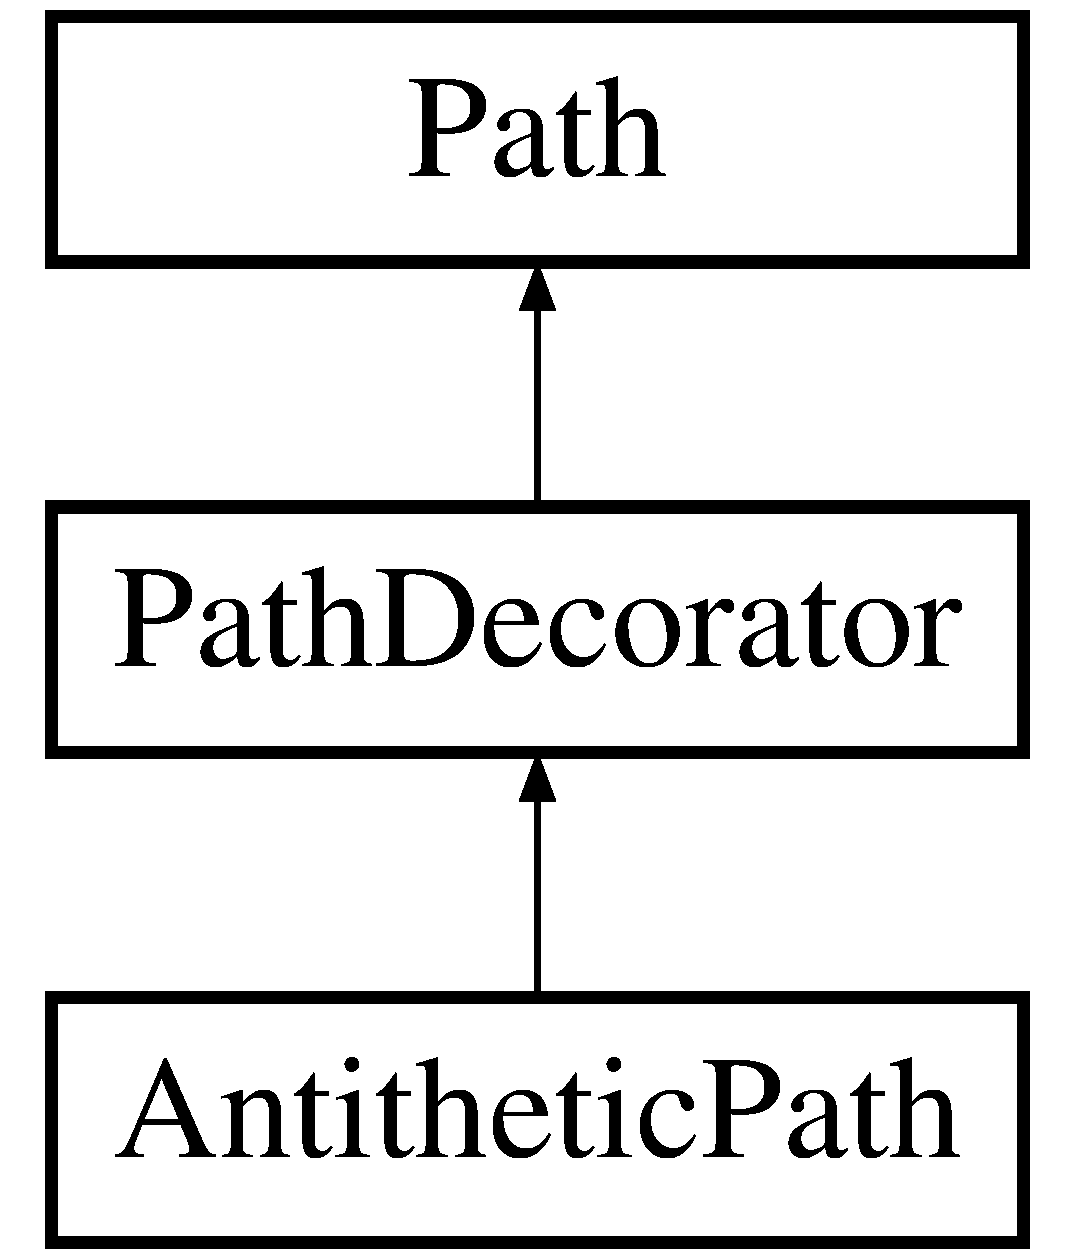
\includegraphics[height=3.000000cm]{class_path_decorator}
\end{center}
\end{figure}
\subsection*{Public Member Functions}
\begin{DoxyCompactItemize}
\item 
\hyperlink{class_path_decorator_a11d7b37b1c60bc36e26609ff96e0e329}{Path\+Decorator} ()=default
\item 
\hyperlink{class_path_decorator_a26a8109e1d038f59140a243f1ceb6084}{Path\+Decorator} (std\+::unique\+\_\+ptr$<$ \hyperlink{class_path}{Path} $>$ \&\&inner\+Path)
\end{DoxyCompactItemize}
\subsection*{Protected Attributes}
\begin{DoxyCompactItemize}
\item 
std\+::unique\+\_\+ptr$<$ \hyperlink{class_path}{Path} $>$ \hyperlink{class_path_decorator_a91f1257f216052a32b4ea78feb9d0755}{inner\+Path\+\_\+}
\end{DoxyCompactItemize}


\subsection{Constructor \& Destructor Documentation}
\hypertarget{class_path_decorator_a11d7b37b1c60bc36e26609ff96e0e329}{}\label{class_path_decorator_a11d7b37b1c60bc36e26609ff96e0e329} 
\index{Path\+Decorator@{Path\+Decorator}!Path\+Decorator@{Path\+Decorator}}
\index{Path\+Decorator@{Path\+Decorator}!Path\+Decorator@{Path\+Decorator}}
\subsubsection{\texorpdfstring{Path\+Decorator()}{PathDecorator()}\hspace{0.1cm}{\footnotesize\ttfamily [1/2]}}
{\footnotesize\ttfamily Path\+Decorator\+::\+Path\+Decorator (\begin{DoxyParamCaption}{ }\end{DoxyParamCaption})\hspace{0.3cm}{\ttfamily [default]}}

\hypertarget{class_path_decorator_a26a8109e1d038f59140a243f1ceb6084}{}\label{class_path_decorator_a26a8109e1d038f59140a243f1ceb6084} 
\index{Path\+Decorator@{Path\+Decorator}!Path\+Decorator@{Path\+Decorator}}
\index{Path\+Decorator@{Path\+Decorator}!Path\+Decorator@{Path\+Decorator}}
\subsubsection{\texorpdfstring{Path\+Decorator()}{PathDecorator()}\hspace{0.1cm}{\footnotesize\ttfamily [2/2]}}
{\footnotesize\ttfamily Path\+Decorator\+::\+Path\+Decorator (\begin{DoxyParamCaption}\item[{std\+::unique\+\_\+ptr$<$ \hyperlink{class_path}{Path} $>$ \&\&}]{inner\+Path }\end{DoxyParamCaption})\hspace{0.3cm}{\ttfamily [inline]}}



\subsection{Member Data Documentation}
\hypertarget{class_path_decorator_a91f1257f216052a32b4ea78feb9d0755}{}\label{class_path_decorator_a91f1257f216052a32b4ea78feb9d0755} 
\index{Path\+Decorator@{Path\+Decorator}!inner\+Path\+\_\+@{inner\+Path\+\_\+}}
\index{inner\+Path\+\_\+@{inner\+Path\+\_\+}!Path\+Decorator@{Path\+Decorator}}
\subsubsection{\texorpdfstring{inner\+Path\+\_\+}{innerPath\_}}
{\footnotesize\ttfamily std\+::unique\+\_\+ptr$<$\hyperlink{class_path}{Path}$>$ Path\+Decorator\+::inner\+Path\+\_\+\hspace{0.3cm}{\ttfamily [protected]}}



The documentation for this class was generated from the following file\+:\begin{DoxyCompactItemize}
\item 
Users/\+C\+U\+I/\+Dropbox/\+C++/\+Finance/\+Mc\+Framework/\hyperlink{_path_8h}{Path.\+h}\end{DoxyCompactItemize}

\hypertarget{class_path_generator}{}\section{Path\+Generator$<$ R\+NG $>$ Class Template Reference}
\label{class_path_generator}\index{Path\+Generator$<$ R\+N\+G $>$@{Path\+Generator$<$ R\+N\+G $>$}}


{\ttfamily \#include $<$Path\+Generator.\+h$>$}

\subsection*{Public Member Functions}
\begin{DoxyCompactItemize}
\item 
\hyperlink{class_path_generator_a7cd1bbe2d0d6afc8b7a6b812553deacc}{Path\+Generator} (const std\+::shared\+\_\+ptr$<$ \hyperlink{class_model}{Model} $>$ model, const vector$<$ \hyperlink{_name_def_8h_ac2d3e0ba793497bcca555c7c2cf64ff3}{Time} $>$ \&time\+Grid, R\+NG rng, bool is\+Antithetic=0)
\item 
\hyperlink{class_path}{Path} \& \hyperlink{class_path_generator_a848a4f432d86df5b03d835d99472ab37}{next} ()
\end{DoxyCompactItemize}
\subsection*{Private Attributes}
\begin{DoxyCompactItemize}
\item 
R\+NG \hyperlink{class_path_generator_ae8b29fa9173cf38dfc448375163adf25}{rng\+\_\+}
\item 
std\+::shared\+\_\+ptr$<$ \hyperlink{class_model}{Model} $>$ \hyperlink{class_path_generator_a80dcaacd0b79c84c4bf83e980f5ed7ff}{model\+\_\+}
\item 
std\+::shared\+\_\+ptr$<$ \hyperlink{class_path}{Path} $>$ \hyperlink{class_path_generator_a2af5b3cab0498565a56b20e97a3d6f35}{next\+\_\+}
\item 
bool \hyperlink{class_path_generator_aa45100f04c27cd0f25c059c410316346}{is\+Antithetic\+\_\+}
\end{DoxyCompactItemize}


\subsection{Constructor \& Destructor Documentation}
\hypertarget{class_path_generator_a7cd1bbe2d0d6afc8b7a6b812553deacc}{}\label{class_path_generator_a7cd1bbe2d0d6afc8b7a6b812553deacc} 
\index{Path\+Generator@{Path\+Generator}!Path\+Generator@{Path\+Generator}}
\index{Path\+Generator@{Path\+Generator}!Path\+Generator@{Path\+Generator}}
\subsubsection{\texorpdfstring{Path\+Generator()}{PathGenerator()}}
{\footnotesize\ttfamily template$<$typename R\+NG $>$ \\
\hyperlink{class_path_generator}{Path\+Generator}$<$ R\+NG $>$\+::\hyperlink{class_path_generator}{Path\+Generator} (\begin{DoxyParamCaption}\item[{const std\+::shared\+\_\+ptr$<$ \hyperlink{class_model}{Model} $>$}]{model,  }\item[{const vector$<$ \hyperlink{_name_def_8h_ac2d3e0ba793497bcca555c7c2cf64ff3}{Time} $>$ \&}]{time\+Grid,  }\item[{R\+NG}]{rng,  }\item[{bool}]{is\+Antithetic = {\ttfamily 0} }\end{DoxyParamCaption})}

!! dimension problem appeared here !!! should be implied by process/path\+Pricer 

\subsection{Member Function Documentation}
\hypertarget{class_path_generator_a848a4f432d86df5b03d835d99472ab37}{}\label{class_path_generator_a848a4f432d86df5b03d835d99472ab37} 
\index{Path\+Generator@{Path\+Generator}!next@{next}}
\index{next@{next}!Path\+Generator@{Path\+Generator}}
\subsubsection{\texorpdfstring{next()}{next()}}
{\footnotesize\ttfamily template$<$typename R\+NG $>$ \\
\hyperlink{class_path}{Path} \& \hyperlink{class_path_generator}{Path\+Generator}$<$ R\+NG $>$\+::next (\begin{DoxyParamCaption}{ }\end{DoxyParamCaption})}



\subsection{Member Data Documentation}
\hypertarget{class_path_generator_aa45100f04c27cd0f25c059c410316346}{}\label{class_path_generator_aa45100f04c27cd0f25c059c410316346} 
\index{Path\+Generator@{Path\+Generator}!is\+Antithetic\+\_\+@{is\+Antithetic\+\_\+}}
\index{is\+Antithetic\+\_\+@{is\+Antithetic\+\_\+}!Path\+Generator@{Path\+Generator}}
\subsubsection{\texorpdfstring{is\+Antithetic\+\_\+}{isAntithetic\_}}
{\footnotesize\ttfamily template$<$typename R\+NG $>$ \\
bool \hyperlink{class_path_generator}{Path\+Generator}$<$ R\+NG $>$\+::is\+Antithetic\+\_\+\hspace{0.3cm}{\ttfamily [private]}}

\hypertarget{class_path_generator_a80dcaacd0b79c84c4bf83e980f5ed7ff}{}\label{class_path_generator_a80dcaacd0b79c84c4bf83e980f5ed7ff} 
\index{Path\+Generator@{Path\+Generator}!model\+\_\+@{model\+\_\+}}
\index{model\+\_\+@{model\+\_\+}!Path\+Generator@{Path\+Generator}}
\subsubsection{\texorpdfstring{model\+\_\+}{model\_}}
{\footnotesize\ttfamily template$<$typename R\+NG $>$ \\
std\+::shared\+\_\+ptr$<$\hyperlink{class_model}{Model}$>$ \hyperlink{class_path_generator}{Path\+Generator}$<$ R\+NG $>$\+::model\+\_\+\hspace{0.3cm}{\ttfamily [private]}}

\hypertarget{class_path_generator_a2af5b3cab0498565a56b20e97a3d6f35}{}\label{class_path_generator_a2af5b3cab0498565a56b20e97a3d6f35} 
\index{Path\+Generator@{Path\+Generator}!next\+\_\+@{next\+\_\+}}
\index{next\+\_\+@{next\+\_\+}!Path\+Generator@{Path\+Generator}}
\subsubsection{\texorpdfstring{next\+\_\+}{next\_}}
{\footnotesize\ttfamily template$<$typename R\+NG $>$ \\
std\+::shared\+\_\+ptr$<$\hyperlink{class_path}{Path}$>$ \hyperlink{class_path_generator}{Path\+Generator}$<$ R\+NG $>$\+::next\+\_\+\hspace{0.3cm}{\ttfamily [private]}}

\hypertarget{class_path_generator_ae8b29fa9173cf38dfc448375163adf25}{}\label{class_path_generator_ae8b29fa9173cf38dfc448375163adf25} 
\index{Path\+Generator@{Path\+Generator}!rng\+\_\+@{rng\+\_\+}}
\index{rng\+\_\+@{rng\+\_\+}!Path\+Generator@{Path\+Generator}}
\subsubsection{\texorpdfstring{rng\+\_\+}{rng\_}}
{\footnotesize\ttfamily template$<$typename R\+NG $>$ \\
R\+NG \hyperlink{class_path_generator}{Path\+Generator}$<$ R\+NG $>$\+::rng\+\_\+\hspace{0.3cm}{\ttfamily [private]}}



The documentation for this class was generated from the following file\+:\begin{DoxyCompactItemize}
\item 
Users/\+C\+U\+I/\+Dropbox/\+C++/\+Finance/\+Mc\+Framework/\hyperlink{_path_generator_8h}{Path\+Generator.\+h}\end{DoxyCompactItemize}

\hypertarget{class_path_pricer}{}\section{Path\+Pricer$<$ Path\+Type $>$ Class Template Reference}
\label{class_path_pricer}\index{Path\+Pricer$<$ Path\+Type $>$@{Path\+Pricer$<$ Path\+Type $>$}}


{\ttfamily \#include $<$Path\+Pricer.\+h$>$}

\subsection*{Public Member Functions}
\begin{DoxyCompactItemize}
\item 
virtual \hyperlink{_name_def_8h_a5a9d48c16a694e9a2d9f1eca730dc8c5}{Money} \hyperlink{class_path_pricer_a14b2a03f259bb56a24a66c9b95bdcf67}{operator()} (const \hyperlink{class_path}{Path}$<$ Path\+Type $>$ \&path) const =0
\end{DoxyCompactItemize}


\subsection{Member Function Documentation}
\hypertarget{class_path_pricer_a14b2a03f259bb56a24a66c9b95bdcf67}{}\label{class_path_pricer_a14b2a03f259bb56a24a66c9b95bdcf67} 
\index{Path\+Pricer@{Path\+Pricer}!operator()@{operator()}}
\index{operator()@{operator()}!Path\+Pricer@{Path\+Pricer}}
\subsubsection{\texorpdfstring{operator()()}{operator()()}}
{\footnotesize\ttfamily template$<$typename Path\+Type$>$ \\
virtual \hyperlink{_name_def_8h_a5a9d48c16a694e9a2d9f1eca730dc8c5}{Money} \hyperlink{class_path_pricer}{Path\+Pricer}$<$ Path\+Type $>$\+::operator() (\begin{DoxyParamCaption}\item[{const \hyperlink{class_path}{Path}$<$ Path\+Type $>$ \&}]{path }\end{DoxyParamCaption}) const\hspace{0.3cm}{\ttfamily [pure virtual]}}



Implemented in \hyperlink{class_asian_path_pricer_a929e8a33447f977bfc947e1d5344e353}{Asian\+Path\+Pricer}, and \hyperlink{class_european_path_pricer_a879d161eeff532f1f3e2fc5224b3361b}{European\+Path\+Pricer}.



The documentation for this class was generated from the following file\+:\begin{DoxyCompactItemize}
\item 
Mc\+Framework/\hyperlink{_path_pricer_8h}{Path\+Pricer.\+h}\end{DoxyCompactItemize}

\hypertarget{class_payoff}{}\section{Payoff Class Reference}
\label{class_payoff}\index{Payoff@{Payoff}}


{\ttfamily \#include $<$payoff.\+h$>$}

Inheritance diagram for Payoff\+:\begin{figure}[H]
\begin{center}
\leavevmode
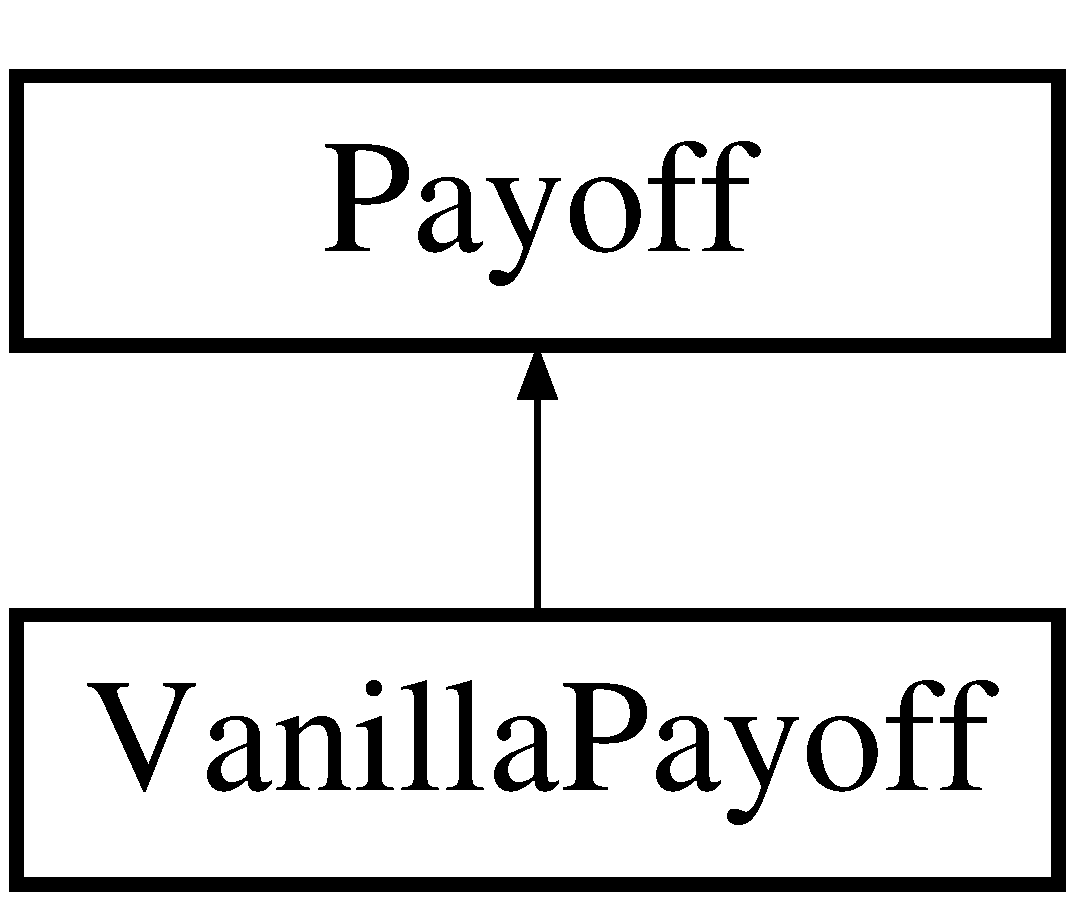
\includegraphics[height=2.000000cm]{class_payoff}
\end{center}
\end{figure}
\subsection*{Public Member Functions}
\begin{DoxyCompactItemize}
\item 
virtual \hyperlink{_name_def_8h_a5a9d48c16a694e9a2d9f1eca730dc8c5}{Money} \hyperlink{class_payoff_a908e732330294a111345b4183ddb025b}{get\+Payoff} (\hyperlink{_name_def_8h_a642a6c5fd87319d922637de0e0bb0305}{Quote} spot) const =0
\end{DoxyCompactItemize}


\subsection{Member Function Documentation}
\hypertarget{class_payoff_a908e732330294a111345b4183ddb025b}{}\label{class_payoff_a908e732330294a111345b4183ddb025b} 
\index{Payoff@{Payoff}!get\+Payoff@{get\+Payoff}}
\index{get\+Payoff@{get\+Payoff}!Payoff@{Payoff}}
\subsubsection{\texorpdfstring{get\+Payoff()}{getPayoff()}}
{\footnotesize\ttfamily virtual \hyperlink{_name_def_8h_a5a9d48c16a694e9a2d9f1eca730dc8c5}{Money} Payoff\+::get\+Payoff (\begin{DoxyParamCaption}\item[{\hyperlink{_name_def_8h_a642a6c5fd87319d922637de0e0bb0305}{Quote}}]{spot }\end{DoxyParamCaption}) const\hspace{0.3cm}{\ttfamily [pure virtual]}}



Implemented in \hyperlink{class_vanilla_payoff_aa141f5b29c30d54448c93a21bef83bb3}{Vanilla\+Payoff}.



The documentation for this class was generated from the following file\+:\begin{DoxyCompactItemize}
\item 
\hyperlink{payoff_8h}{payoff.\+h}\end{DoxyCompactItemize}

\hypertarget{class_pricing_engine}{}\section{Pricing\+Engine Class Reference}
\label{class_pricing_engine}\index{Pricing\+Engine@{Pricing\+Engine}}


{\ttfamily \#include $<$Pricing\+Engine.\+h$>$}

Inheritance diagram for Pricing\+Engine\+:\begin{figure}[H]
\begin{center}
\leavevmode
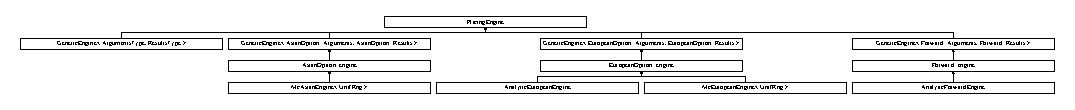
\includegraphics[height=1.034642cm]{class_pricing_engine}
\end{center}
\end{figure}
\subsection*{Classes}
\begin{DoxyCompactItemize}
\item 
class \hyperlink{class_pricing_engine_1_1_arguments}{Arguments}
\item 
class \hyperlink{class_pricing_engine_1_1_results}{Results}
\end{DoxyCompactItemize}
\subsection*{Public Member Functions}
\begin{DoxyCompactItemize}
\item 
\hyperlink{class_pricing_engine_abfd32778b0483e92db2e7cd00a2f9345}{Pricing\+Engine} ()
\item 
virtual void \hyperlink{class_pricing_engine_a733511ffc3cf5e4dc1fbc2a39208d8bd}{calculate} ()=0
\item 
virtual \hyperlink{class_pricing_engine_1_1_arguments}{Arguments} $\ast$ \hyperlink{class_pricing_engine_a399f4519f58b2ac1d108ce14d0058c97}{get\+Arguments} () const =0
\item 
virtual \hyperlink{class_pricing_engine_1_1_results}{Results} $\ast$ \hyperlink{class_pricing_engine_a73e2852ef4c28e92a402492e86717d0b}{get\+Results} () const =0
\end{DoxyCompactItemize}


\subsection{Constructor \& Destructor Documentation}
\hypertarget{class_pricing_engine_abfd32778b0483e92db2e7cd00a2f9345}{}\label{class_pricing_engine_abfd32778b0483e92db2e7cd00a2f9345} 
\index{Pricing\+Engine@{Pricing\+Engine}!Pricing\+Engine@{Pricing\+Engine}}
\index{Pricing\+Engine@{Pricing\+Engine}!Pricing\+Engine@{Pricing\+Engine}}
\subsubsection{\texorpdfstring{Pricing\+Engine()}{PricingEngine()}}
{\footnotesize\ttfamily Pricing\+Engine\+::\+Pricing\+Engine (\begin{DoxyParamCaption}{ }\end{DoxyParamCaption})\hspace{0.3cm}{\ttfamily [inline]}}



\subsection{Member Function Documentation}
\hypertarget{class_pricing_engine_a733511ffc3cf5e4dc1fbc2a39208d8bd}{}\label{class_pricing_engine_a733511ffc3cf5e4dc1fbc2a39208d8bd} 
\index{Pricing\+Engine@{Pricing\+Engine}!calculate@{calculate}}
\index{calculate@{calculate}!Pricing\+Engine@{Pricing\+Engine}}
\subsubsection{\texorpdfstring{calculate()}{calculate()}}
{\footnotesize\ttfamily virtual void Pricing\+Engine\+::calculate (\begin{DoxyParamCaption}{ }\end{DoxyParamCaption})\hspace{0.3cm}{\ttfamily [pure virtual]}}



Implemented in \hyperlink{class_mc_european_engine_a51b2f0147fbaf2b84c65851bbc2baa7b}{Mc\+European\+Engine$<$ Unif\+Rng $>$}, \hyperlink{class_mc_asian_engine_a4e67149307de395f821c8aa07afad3b8}{Mc\+Asian\+Engine$<$ Unif\+Rng $>$}, \hyperlink{class_analytic_european_engine_adeda22c7b482779d7deaa17037195487}{Analytic\+European\+Engine}, and \hyperlink{class_analytic_forward_engine_a12d6791a13bf727d43ffcff9cb55b094}{Analytic\+Forward\+Engine}.

\hypertarget{class_pricing_engine_a399f4519f58b2ac1d108ce14d0058c97}{}\label{class_pricing_engine_a399f4519f58b2ac1d108ce14d0058c97} 
\index{Pricing\+Engine@{Pricing\+Engine}!get\+Arguments@{get\+Arguments}}
\index{get\+Arguments@{get\+Arguments}!Pricing\+Engine@{Pricing\+Engine}}
\subsubsection{\texorpdfstring{get\+Arguments()}{getArguments()}}
{\footnotesize\ttfamily virtual \hyperlink{class_pricing_engine_1_1_arguments}{Arguments}$\ast$ Pricing\+Engine\+::get\+Arguments (\begin{DoxyParamCaption}{ }\end{DoxyParamCaption}) const\hspace{0.3cm}{\ttfamily [pure virtual]}}



Implemented in \hyperlink{class_generic_engine_ac2adcbbc8d7b554e2cc1f90e4c4d055d}{Generic\+Engine$<$ Arguments\+Type, Results\+Type $>$}, \hyperlink{class_generic_engine_ac2adcbbc8d7b554e2cc1f90e4c4d055d}{Generic\+Engine$<$ European\+Option\+::\+Arguments, European\+Option\+::\+Results $>$}, \hyperlink{class_generic_engine_ac2adcbbc8d7b554e2cc1f90e4c4d055d}{Generic\+Engine$<$ Asian\+Option\+::\+Arguments, Asian\+Option\+::\+Results $>$}, and \hyperlink{class_generic_engine_ac2adcbbc8d7b554e2cc1f90e4c4d055d}{Generic\+Engine$<$ Forward\+::\+Arguments, Forward\+::\+Results $>$}.

\hypertarget{class_pricing_engine_a73e2852ef4c28e92a402492e86717d0b}{}\label{class_pricing_engine_a73e2852ef4c28e92a402492e86717d0b} 
\index{Pricing\+Engine@{Pricing\+Engine}!get\+Results@{get\+Results}}
\index{get\+Results@{get\+Results}!Pricing\+Engine@{Pricing\+Engine}}
\subsubsection{\texorpdfstring{get\+Results()}{getResults()}}
{\footnotesize\ttfamily virtual \hyperlink{class_pricing_engine_1_1_results}{Results}$\ast$ Pricing\+Engine\+::get\+Results (\begin{DoxyParamCaption}{ }\end{DoxyParamCaption}) const\hspace{0.3cm}{\ttfamily [pure virtual]}}



Implemented in \hyperlink{class_generic_engine_a2b8d7fba7e51c0795ea9f1e9c2f54afd}{Generic\+Engine$<$ Arguments\+Type, Results\+Type $>$}, \hyperlink{class_generic_engine_a2b8d7fba7e51c0795ea9f1e9c2f54afd}{Generic\+Engine$<$ European\+Option\+::\+Arguments, European\+Option\+::\+Results $>$}, \hyperlink{class_generic_engine_a2b8d7fba7e51c0795ea9f1e9c2f54afd}{Generic\+Engine$<$ Asian\+Option\+::\+Arguments, Asian\+Option\+::\+Results $>$}, and \hyperlink{class_generic_engine_a2b8d7fba7e51c0795ea9f1e9c2f54afd}{Generic\+Engine$<$ Forward\+::\+Arguments, Forward\+::\+Results $>$}.



The documentation for this class was generated from the following file\+:\begin{DoxyCompactItemize}
\item 
Users/\+C\+U\+I/\+Dropbox/\+C++/\+Finance/\hyperlink{_pricing_engine_8h}{Pricing\+Engine.\+h}\end{DoxyCompactItemize}

\hypertarget{class_random_sequence_generator}{}\section{Random\+Sequence\+Generator$<$ R\+NG $>$ Class Template Reference}
\label{class_random_sequence_generator}\index{Random\+Sequence\+Generator$<$ R\+N\+G $>$@{Random\+Sequence\+Generator$<$ R\+N\+G $>$}}
\subsection*{Public Member Functions}
\begin{DoxyCompactItemize}
\item 
\hypertarget{class_random_sequence_generator_a148644138c29dae6ebe57657c8ca2cce}{}\label{class_random_sequence_generator_a148644138c29dae6ebe57657c8ca2cce} 
{\bfseries Random\+Sequence\+Generator} (vector$<$ double $>$\+::size\+\_\+type dimensionality, const R\+NG \&rng)
\item 
\hypertarget{class_random_sequence_generator_a63f2d6fdb7f7bab6cdf3506f91cc814c}{}\label{class_random_sequence_generator_a63f2d6fdb7f7bab6cdf3506f91cc814c} 
const vector$<$ double $>$ \& {\bfseries next\+Sequence} ()
\end{DoxyCompactItemize}


The documentation for this class was generated from the following file\+:\begin{DoxyCompactItemize}
\item 
Users/\+C\+U\+I/\+Dropbox/\+C++/\+Finance/\+Rand\+Num\+Generation/Random\+Sequence\+Generator.\+h\end{DoxyCompactItemize}

\hypertarget{class_european_option_1_1_results}{}\section{European\+Option\+:\+:Results Class Reference}
\label{class_european_option_1_1_results}\index{European\+Option\+::\+Results@{European\+Option\+::\+Results}}


{\ttfamily \#include $<$European\+Option.\+h$>$}

Inheritance diagram for European\+Option\+:\+:Results\+:\begin{figure}[H]
\begin{center}
\leavevmode
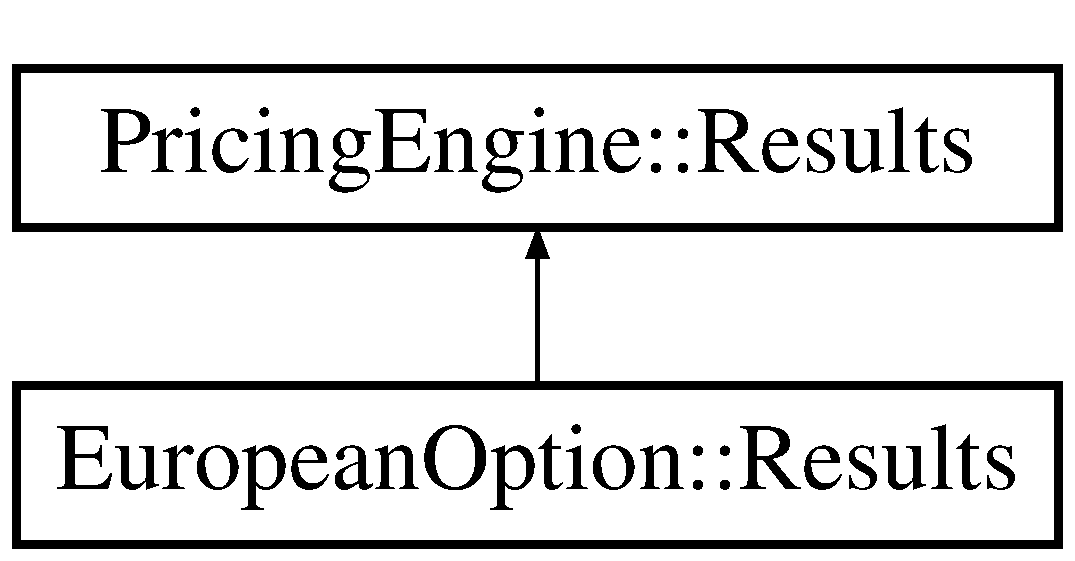
\includegraphics[height=2.000000cm]{class_european_option_1_1_results}
\end{center}
\end{figure}
\subsection*{Public Attributes}
\begin{DoxyCompactItemize}
\item 
\hyperlink{_name_def_8h_a5a9d48c16a694e9a2d9f1eca730dc8c5}{Money} \hyperlink{class_european_option_1_1_results_a517b87143fda866b135b21051dc4fd6c}{price\+\_\+}
\item 
double \hyperlink{class_european_option_1_1_results_a3e9ddb58f8e1f69b972bfed5e893414b}{delta\+\_\+}
\end{DoxyCompactItemize}
\subsection*{Additional Inherited Members}


\subsection{Member Data Documentation}
\hypertarget{class_european_option_1_1_results_a3e9ddb58f8e1f69b972bfed5e893414b}{}\label{class_european_option_1_1_results_a3e9ddb58f8e1f69b972bfed5e893414b} 
\index{European\+Option\+::\+Results@{European\+Option\+::\+Results}!delta\+\_\+@{delta\+\_\+}}
\index{delta\+\_\+@{delta\+\_\+}!European\+Option\+::\+Results@{European\+Option\+::\+Results}}
\subsubsection{\texorpdfstring{delta\+\_\+}{delta\_}}
{\footnotesize\ttfamily double European\+Option\+::\+Results\+::delta\+\_\+}

\hypertarget{class_european_option_1_1_results_a517b87143fda866b135b21051dc4fd6c}{}\label{class_european_option_1_1_results_a517b87143fda866b135b21051dc4fd6c} 
\index{European\+Option\+::\+Results@{European\+Option\+::\+Results}!price\+\_\+@{price\+\_\+}}
\index{price\+\_\+@{price\+\_\+}!European\+Option\+::\+Results@{European\+Option\+::\+Results}}
\subsubsection{\texorpdfstring{price\+\_\+}{price\_}}
{\footnotesize\ttfamily \hyperlink{_name_def_8h_a5a9d48c16a694e9a2d9f1eca730dc8c5}{Money} European\+Option\+::\+Results\+::price\+\_\+}



The documentation for this class was generated from the following file\+:\begin{DoxyCompactItemize}
\item 
Users/\+C\+U\+I/\+Dropbox/\+C++/\+Finance/\+Instruments/\hyperlink{_european_option_8h}{European\+Option.\+h}\end{DoxyCompactItemize}

\hypertarget{class_pricing_engine_1_1_results}{}\section{Pricing\+Engine\+:\+:Results Class Reference}
\label{class_pricing_engine_1_1_results}\index{Pricing\+Engine\+::\+Results@{Pricing\+Engine\+::\+Results}}


{\ttfamily \#include $<$Pricing\+Engine.\+h$>$}

Inheritance diagram for Pricing\+Engine\+:\+:Results\+:\begin{figure}[H]
\begin{center}
\leavevmode
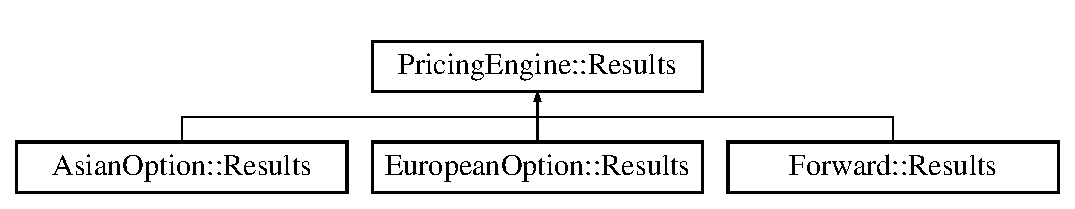
\includegraphics[height=2.000000cm]{class_pricing_engine_1_1_results}
\end{center}
\end{figure}
\subsection*{Public Member Functions}
\begin{DoxyCompactItemize}
\item 
\hyperlink{class_pricing_engine_1_1_results_a2bbf5c82ee43b77905a06659f26f3bf0}{Results} ()
\item 
virtual \hyperlink{class_pricing_engine_1_1_results_a3a0c59acadf917438c07697f547de53e}{$\sim$\+Results} ()
\end{DoxyCompactItemize}


\subsection{Constructor \& Destructor Documentation}
\hypertarget{class_pricing_engine_1_1_results_a2bbf5c82ee43b77905a06659f26f3bf0}{}\label{class_pricing_engine_1_1_results_a2bbf5c82ee43b77905a06659f26f3bf0} 
\index{Pricing\+Engine\+::\+Results@{Pricing\+Engine\+::\+Results}!Results@{Results}}
\index{Results@{Results}!Pricing\+Engine\+::\+Results@{Pricing\+Engine\+::\+Results}}
\subsubsection{\texorpdfstring{Results()}{Results()}}
{\footnotesize\ttfamily Pricing\+Engine\+::\+Results\+::\+Results (\begin{DoxyParamCaption}{ }\end{DoxyParamCaption})\hspace{0.3cm}{\ttfamily [inline]}}

\hypertarget{class_pricing_engine_1_1_results_a3a0c59acadf917438c07697f547de53e}{}\label{class_pricing_engine_1_1_results_a3a0c59acadf917438c07697f547de53e} 
\index{Pricing\+Engine\+::\+Results@{Pricing\+Engine\+::\+Results}!````~Results@{$\sim$\+Results}}
\index{````~Results@{$\sim$\+Results}!Pricing\+Engine\+::\+Results@{Pricing\+Engine\+::\+Results}}
\subsubsection{\texorpdfstring{$\sim$\+Results()}{~Results()}}
{\footnotesize\ttfamily virtual Pricing\+Engine\+::\+Results\+::$\sim$\+Results (\begin{DoxyParamCaption}{ }\end{DoxyParamCaption})\hspace{0.3cm}{\ttfamily [inline]}, {\ttfamily [virtual]}}



The documentation for this class was generated from the following file\+:\begin{DoxyCompactItemize}
\item 
\hyperlink{_pricing_engine_8h}{Pricing\+Engine.\+h}\end{DoxyCompactItemize}

\hypertarget{class_forward_1_1_results}{}\section{Forward\+:\+:Results Class Reference}
\label{class_forward_1_1_results}\index{Forward\+::\+Results@{Forward\+::\+Results}}


{\ttfamily \#include $<$Forward.\+h$>$}

Inheritance diagram for Forward\+:\+:Results\+:\begin{figure}[H]
\begin{center}
\leavevmode
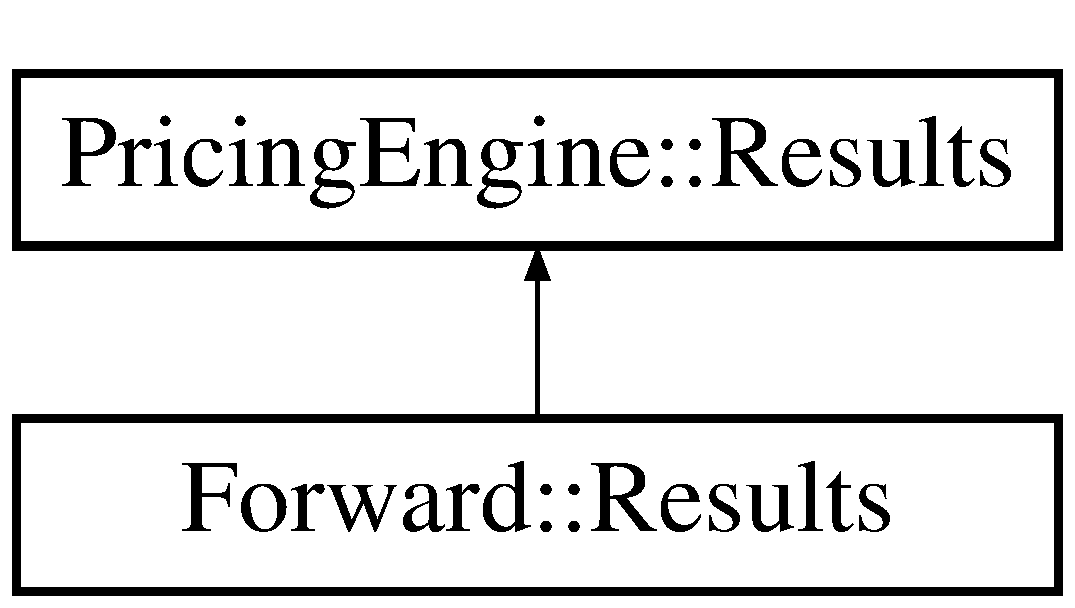
\includegraphics[height=2.000000cm]{class_forward_1_1_results}
\end{center}
\end{figure}
\subsection*{Public Attributes}
\begin{DoxyCompactItemize}
\item 
\hyperlink{_name_def_8h_a5a9d48c16a694e9a2d9f1eca730dc8c5}{Money} \hyperlink{class_forward_1_1_results_a61aa9829fa13483ef961836334e1d473}{price\+\_\+}
\end{DoxyCompactItemize}
\subsection*{Additional Inherited Members}


\subsection{Member Data Documentation}
\hypertarget{class_forward_1_1_results_a61aa9829fa13483ef961836334e1d473}{}\label{class_forward_1_1_results_a61aa9829fa13483ef961836334e1d473} 
\index{Forward\+::\+Results@{Forward\+::\+Results}!price\+\_\+@{price\+\_\+}}
\index{price\+\_\+@{price\+\_\+}!Forward\+::\+Results@{Forward\+::\+Results}}
\subsubsection{\texorpdfstring{price\+\_\+}{price\_}}
{\footnotesize\ttfamily \hyperlink{_name_def_8h_a5a9d48c16a694e9a2d9f1eca730dc8c5}{Money} Forward\+::\+Results\+::price\+\_\+}



The documentation for this class was generated from the following file\+:\begin{DoxyCompactItemize}
\item 
Users/\+C\+U\+I/\+Dropbox/\+C++/\+Finance/\+Instruments/\hyperlink{_forward_8h}{Forward.\+h}\end{DoxyCompactItemize}

\hypertarget{class_asian_option_1_1_results}{}\section{Asian\+Option\+:\+:Results Class Reference}
\label{class_asian_option_1_1_results}\index{Asian\+Option\+::\+Results@{Asian\+Option\+::\+Results}}


Result class of Asian option Accessory class which is used to interact with pricing engine.  




{\ttfamily \#include $<$Asian\+Option.\+h$>$}

Inheritance diagram for Asian\+Option\+:\+:Results\+:\begin{figure}[H]
\begin{center}
\leavevmode
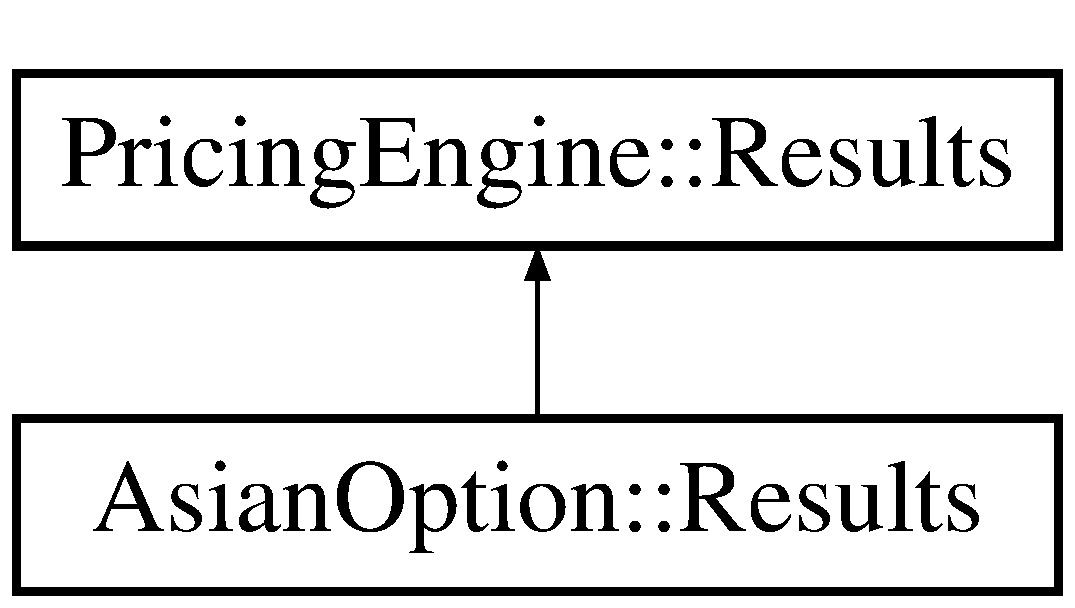
\includegraphics[height=2.000000cm]{class_asian_option_1_1_results}
\end{center}
\end{figure}
\subsection*{Public Attributes}
\begin{DoxyCompactItemize}
\item 
\hyperlink{_name_def_8h_a5a9d48c16a694e9a2d9f1eca730dc8c5}{Money} \hyperlink{class_asian_option_1_1_results_a9e4e4e2612f105b940b1562d7f126a89}{price\+\_\+}
\begin{DoxyCompactList}\small\item\em Net present value of Asian option. \end{DoxyCompactList}\end{DoxyCompactItemize}
\subsection*{Additional Inherited Members}


\subsection{Detailed Description}
Result class of Asian option Accessory class which is used to interact with pricing engine. 

~\newline
Inherited from Result class of \hyperlink{class_pricing_engine}{Pricing\+Engine}. 

\subsection{Member Data Documentation}
\hypertarget{class_asian_option_1_1_results_a9e4e4e2612f105b940b1562d7f126a89}{}\label{class_asian_option_1_1_results_a9e4e4e2612f105b940b1562d7f126a89} 
\index{Asian\+Option\+::\+Results@{Asian\+Option\+::\+Results}!price\+\_\+@{price\+\_\+}}
\index{price\+\_\+@{price\+\_\+}!Asian\+Option\+::\+Results@{Asian\+Option\+::\+Results}}
\subsubsection{\texorpdfstring{price\+\_\+}{price\_}}
{\footnotesize\ttfamily \hyperlink{_name_def_8h_a5a9d48c16a694e9a2d9f1eca730dc8c5}{Money} Asian\+Option\+::\+Results\+::price\+\_\+}



Net present value of Asian option. 



The documentation for this class was generated from the following file\+:\begin{DoxyCompactItemize}
\item 
Instruments/\hyperlink{_asian_option_8h}{Asian\+Option.\+h}\end{DoxyCompactItemize}

\hypertarget{class_m_c_statistics_1_1_sample_results}{}\section{M\+C\+Statistics\+:\+:Sample\+Results Class Reference}
\label{class_m_c_statistics_1_1_sample_results}\index{M\+C\+Statistics\+::\+Sample\+Results@{M\+C\+Statistics\+::\+Sample\+Results}}


{\ttfamily \#include $<$Statistics.\+h$>$}

\subsection*{Public Member Functions}
\begin{DoxyCompactItemize}
\item 
\hyperlink{class_m_c_statistics_1_1_sample_results_a49be18ef127e000d7f828ff69813abee}{Sample\+Results} (unsigned long num\+Sample, \hyperlink{_name_def_8h_a5a9d48c16a694e9a2d9f1eca730dc8c5}{Money} price)
\end{DoxyCompactItemize}
\subsection*{Public Attributes}
\begin{DoxyCompactItemize}
\item 
unsigned long \hyperlink{class_m_c_statistics_1_1_sample_results_a068edc7e162d279df3df01df775f431a}{num\+Sample\+\_\+}
\item 
\hyperlink{_name_def_8h_a5a9d48c16a694e9a2d9f1eca730dc8c5}{Money} \hyperlink{class_m_c_statistics_1_1_sample_results_a942ac0f979f34804055ff0f5287516f1}{price\+\_\+}
\end{DoxyCompactItemize}


\subsection{Constructor \& Destructor Documentation}
\hypertarget{class_m_c_statistics_1_1_sample_results_a49be18ef127e000d7f828ff69813abee}{}\label{class_m_c_statistics_1_1_sample_results_a49be18ef127e000d7f828ff69813abee} 
\index{M\+C\+Statistics\+::\+Sample\+Results@{M\+C\+Statistics\+::\+Sample\+Results}!Sample\+Results@{Sample\+Results}}
\index{Sample\+Results@{Sample\+Results}!M\+C\+Statistics\+::\+Sample\+Results@{M\+C\+Statistics\+::\+Sample\+Results}}
\subsubsection{\texorpdfstring{Sample\+Results()}{SampleResults()}}
{\footnotesize\ttfamily M\+C\+Statistics\+::\+Sample\+Results\+::\+Sample\+Results (\begin{DoxyParamCaption}\item[{unsigned long}]{num\+Sample,  }\item[{\hyperlink{_name_def_8h_a5a9d48c16a694e9a2d9f1eca730dc8c5}{Money}}]{price }\end{DoxyParamCaption})\hspace{0.3cm}{\ttfamily [inline]}}



\subsection{Member Data Documentation}
\hypertarget{class_m_c_statistics_1_1_sample_results_a068edc7e162d279df3df01df775f431a}{}\label{class_m_c_statistics_1_1_sample_results_a068edc7e162d279df3df01df775f431a} 
\index{M\+C\+Statistics\+::\+Sample\+Results@{M\+C\+Statistics\+::\+Sample\+Results}!num\+Sample\+\_\+@{num\+Sample\+\_\+}}
\index{num\+Sample\+\_\+@{num\+Sample\+\_\+}!M\+C\+Statistics\+::\+Sample\+Results@{M\+C\+Statistics\+::\+Sample\+Results}}
\subsubsection{\texorpdfstring{num\+Sample\+\_\+}{numSample\_}}
{\footnotesize\ttfamily unsigned long M\+C\+Statistics\+::\+Sample\+Results\+::num\+Sample\+\_\+}

\hypertarget{class_m_c_statistics_1_1_sample_results_a942ac0f979f34804055ff0f5287516f1}{}\label{class_m_c_statistics_1_1_sample_results_a942ac0f979f34804055ff0f5287516f1} 
\index{M\+C\+Statistics\+::\+Sample\+Results@{M\+C\+Statistics\+::\+Sample\+Results}!price\+\_\+@{price\+\_\+}}
\index{price\+\_\+@{price\+\_\+}!M\+C\+Statistics\+::\+Sample\+Results@{M\+C\+Statistics\+::\+Sample\+Results}}
\subsubsection{\texorpdfstring{price\+\_\+}{price\_}}
{\footnotesize\ttfamily \hyperlink{_name_def_8h_a5a9d48c16a694e9a2d9f1eca730dc8c5}{Money} M\+C\+Statistics\+::\+Sample\+Results\+::price\+\_\+}



The documentation for this class was generated from the following file\+:\begin{DoxyCompactItemize}
\item 
Users/\+C\+U\+I/\+Dropbox/\+C++/\+Finance/\hyperlink{_statistics_8h}{Statistics.\+h}\end{DoxyCompactItemize}

\hypertarget{class_stochastic_process}{}\section{Stochastic\+Process Class Reference}
\label{class_stochastic_process}\index{Stochastic\+Process@{Stochastic\+Process}}
Inheritance diagram for Stochastic\+Process\+:\begin{figure}[H]
\begin{center}
\leavevmode
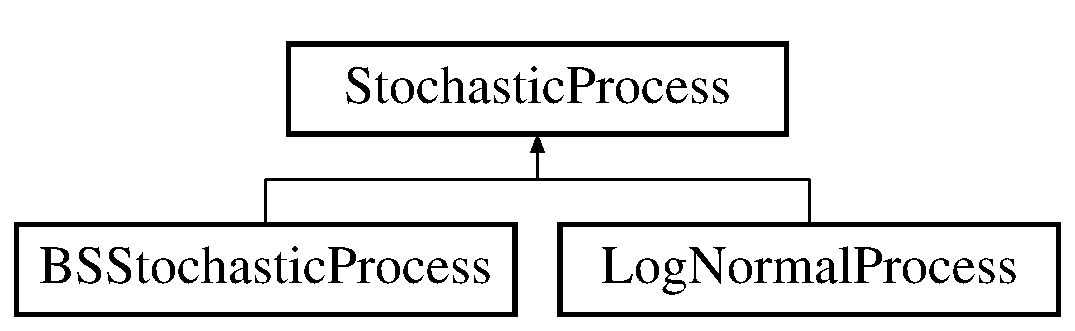
\includegraphics[height=2.000000cm]{class_stochastic_process}
\end{center}
\end{figure}
\subsection*{Classes}
\begin{DoxyCompactItemize}
\item 
class \hyperlink{class_stochastic_process_1_1_parameter_set}{Parameter\+Set}
\end{DoxyCompactItemize}
\subsection*{Public Member Functions}
\begin{DoxyCompactItemize}
\item 
\hypertarget{class_stochastic_process_aad2ef51ca4bc2fe5f33a73e8f0ee361e}{}\label{class_stochastic_process_aad2ef51ca4bc2fe5f33a73e8f0ee361e} 
virtual Quote {\bfseries get\+Spot} () const =0
\end{DoxyCompactItemize}


The documentation for this class was generated from the following file\+:\begin{DoxyCompactItemize}
\item 
Users/\+C\+U\+I/\+Dropbox/\+C++/\+Finance/Stochastic\+Process.\+h\end{DoxyCompactItemize}

\hypertarget{class_uniform_l_ecuyer_r_n_g1}{}\section{Uniform\+L\+Ecuyer\+R\+N\+G1 Class Reference}
\label{class_uniform_l_ecuyer_r_n_g1}\index{Uniform\+L\+Ecuyer\+R\+N\+G1@{Uniform\+L\+Ecuyer\+R\+N\+G1}}
\subsection*{Public Member Functions}
\begin{DoxyCompactItemize}
\item 
\hypertarget{class_uniform_l_ecuyer_r_n_g1_a337fc3fe276e950c8ef9e330779eedb7}{}\label{class_uniform_l_ecuyer_r_n_g1_a337fc3fe276e950c8ef9e330779eedb7} 
{\bfseries Uniform\+L\+Ecuyer\+R\+N\+G1} (unsigned long seed=7777)
\item 
\hypertarget{class_uniform_l_ecuyer_r_n_g1_a33e1ea51eb633a14e84d45d8c31a4e8b}{}\label{class_uniform_l_ecuyer_r_n_g1_a33e1ea51eb633a14e84d45d8c31a4e8b} 
void {\bfseries set\+Seed} (const long seed)
\item 
\hypertarget{class_uniform_l_ecuyer_r_n_g1_a6a166e0bef412d4c85565ec0017ae489}{}\label{class_uniform_l_ecuyer_r_n_g1_a6a166e0bef412d4c85565ec0017ae489} 
double {\bfseries next} ()
\end{DoxyCompactItemize}


The documentation for this class was generated from the following files\+:\begin{DoxyCompactItemize}
\item 
Users/\+C\+U\+I/\+Dropbox/\+C++/\+Finance/\+Rand\+Num\+Generation/Uniform\+L\+Ecuyer\+R\+N\+G1.\+h\item 
Users/\+C\+U\+I/\+Dropbox/\+C++/\+Finance/\+Rand\+Num\+Generation/Uniform\+L\+Ecuyer\+R\+N\+G1.\+cpp\end{DoxyCompactItemize}

\hypertarget{class_vanilla_payoff}{}\section{Vanilla\+Payoff Class Reference}
\label{class_vanilla_payoff}\index{Vanilla\+Payoff@{Vanilla\+Payoff}}
Inheritance diagram for Vanilla\+Payoff\+:\begin{figure}[H]
\begin{center}
\leavevmode
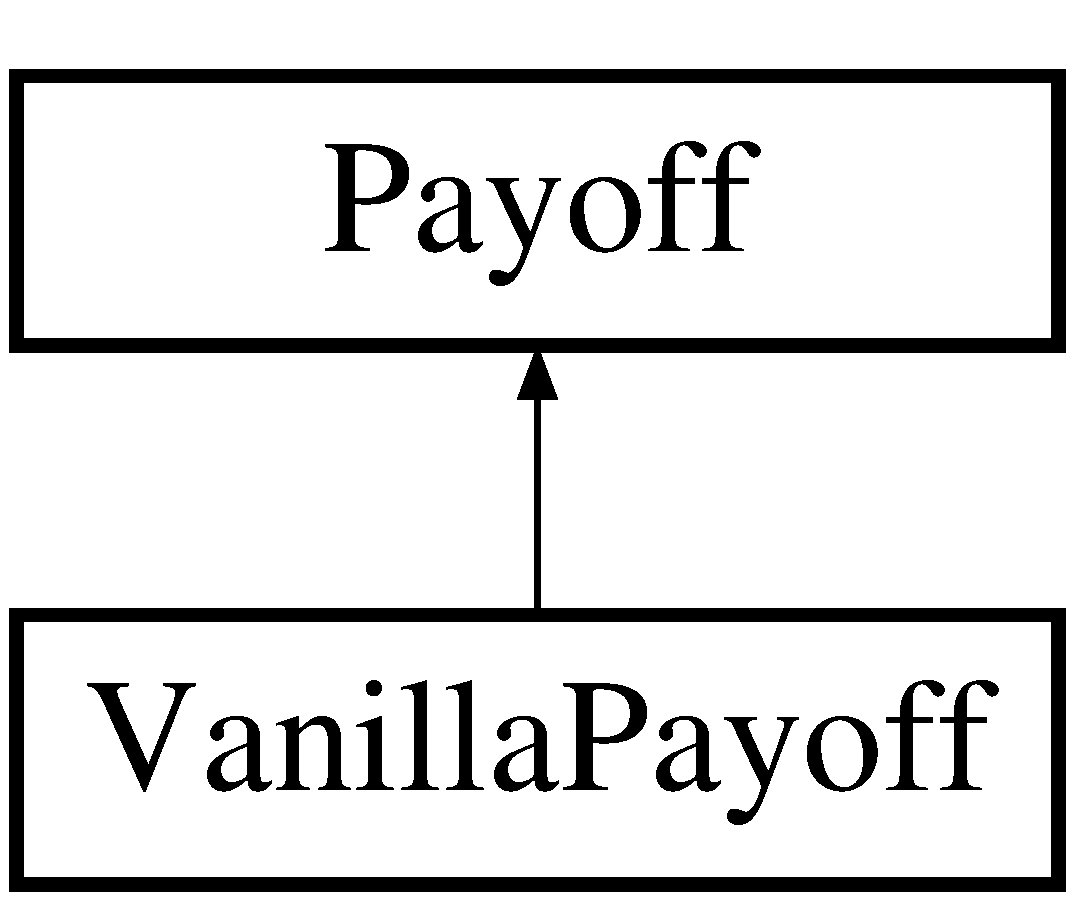
\includegraphics[height=2.000000cm]{class_vanilla_payoff}
\end{center}
\end{figure}
\subsection*{Public Member Functions}
\begin{DoxyCompactItemize}
\item 
\hypertarget{class_vanilla_payoff_ae0d7f1fdb70f4ad9c2002f96df2199d3}{}\label{class_vanilla_payoff_ae0d7f1fdb70f4ad9c2002f96df2199d3} 
{\bfseries Vanilla\+Payoff} (Quote strike, std\+::string type)
\item 
\hypertarget{class_vanilla_payoff_aa141f5b29c30d54448c93a21bef83bb3}{}\label{class_vanilla_payoff_aa141f5b29c30d54448c93a21bef83bb3} 
Money {\bfseries get\+Payoff} (Quote spot) const override
\item 
\hypertarget{class_vanilla_payoff_ae99fb31f1496f723ec598367ece825e3}{}\label{class_vanilla_payoff_ae99fb31f1496f723ec598367ece825e3} 
Quote {\bfseries get\+Strike} () const
\item 
\hypertarget{class_vanilla_payoff_ac1b4cc9e4152ed3f7c07c71270fc1831}{}\label{class_vanilla_payoff_ac1b4cc9e4152ed3f7c07c71270fc1831} 
double {\bfseries get\+Type} () const
\end{DoxyCompactItemize}


The documentation for this class was generated from the following files\+:\begin{DoxyCompactItemize}
\item 
Users/\+C\+U\+I/\+Dropbox/\+C++/\+Finance/\+Payoffs/Vanilla\+Payoff.\+h\item 
Users/\+C\+U\+I/\+Dropbox/\+C++/\+Finance/\+Payoffs/Vanilla\+Payoff.\+cpp\end{DoxyCompactItemize}

%--- End generated contents ---

% Index
\backmatter
\newpage
\phantomsection
\clearemptydoublepage
\addcontentsline{toc}{chapter}{Index}
\printindex

\end{document}
